% Author: Brandon Patterson
% Description: Dissertation
%
%
% Use the University of Michigan thesis class.
\documentclass[submit]{./tex/thesis-umich}


% Title of the thesis
\title{Applications of Computation in Acoustics: Ultrasound Bioeffects and Underwater Transmission Loss Uncertainty}
%\title{Computational investigations of ultrasound bioeffects and related physics}
%\title{Acoustically-driven fluid interfaces with applications to diagnostic ultrasound bioeffects}



% Author name
\author{Brandon Patterson}

% Department
\department{(Mechanical Engineering)}

% Year of completion
\year=\the\year

% Frontispiece
\frontispiece{\includegraphics[width=4in]{./figs/frontispiece/brooke_nobackground}}

% Default style for front pages
\frontpagestyle{1}

%% Dedication
\dedication{\topskip0pt
\pagebreak
\vspace*{\fill}
\begin{center}
  To Dad
\end{center}
\vspace*{\fill}
\pagebreak

%%% Local Variables:
%%% mode: latex
%%% TeX-master: "../main"
%%% End:
}

%% Acknowledgments
\acknowledgments{\include{./content/Acknowledgements}}%

% This command sets the width of the acknowledgments area as a fraction
% of the total width of the text area.
\acknowledgmentswidth{0.75}%

% Preface
%\preface[2]{\include{./content/preface}}%
\preface{\include{./content/preface}}%

% Committee
\committee{%
\hspace*{12pt} Professor David R. Dowling, Co-Chair\\%, Mechanical Engineering, University of Michigan\\
\hspace*{12pt} Associate Professor Eric Johnsen, Co-Chair\\
\hspace*{12pt} Professor J. Brian Fowlkes\\
\hspace*{12pt} Professor Douglas L. Miller\\%, Radiology, University of Michigan
\hspace*{12pt} Professor William Schultz\\%, Mechanical Engineering, University of Michigan\\
}

%% Chair must be entered separately for formatting reasons.
\chair{Eric Johnsen}
\cochair{David R. Dowling \& Eric Johnsen}

%% What deliverable requirement does this fill
\deliverable{Dissertation}

% Commands to hide or show lists of figures, tables, etc.
% \hidelistoftables
% \hidelistofprograms
% \hidelistofappendices
% \hidelistoffigures
% \hidelistofabbreviations
% \hidelistofacronyms
% \hidededication

\showlistoftables
%\showlistofprograms
%\showlistofappendices
\showlistofabbreviations
\showlistoffigures
\showacknowledgments


%% Definition of any abbreviations used.
\abbreviations{
 \acro{CEUS}{Contrast-Enhanced Ultrasound}
 \acro{CFD}{Computational Fluid Dynamics}
 \acro{DG}{Discontinuous Galerkin}
 \acro{DUS}{Diagnostic Ultrasound}
 \acro{HIFU}{High Intensity Focused Ultrasound}
 \acro{IC}{Inertial Cavitation} 
 \acro{LH}{Lung hemorrhage}
 \acro{MC}{Monte Carlo}
 \acro{PD}{Pulse Duration}
 \acro{PDF}{Probability Distribution Function}
 \acro{PFP}{Perfluoropropane}
 \acro{PRF}{Pulse Repetition Frequency}
 \acro{PRPA}{Peak Rarefaction Pressure Amplitude}
 \acro{RMI}{Richtmyer-Meshkov Instability}
 \acro{TL}{Transmission Loss}
 \acro{US}{Ultrasound}


%%% Local Variables:
%%% mode: latex
%%% TeX-master: "../main"
%%% End:

}

%% Some abstract text
%\abstract{\begin{center}
  \begin{minipage}{0.8\textwidth}
    \subsection*{Abstract}
    \ac{DUS} of the lung has been shown to cause hemorrhage in a
    variety of mammals, though the underlying damage mechanism is yet
    to be determined. Motivated by this problem we model an alveolar
    tissue-air interface as a perturbed water-air interface and
    simulate its interaction with trapezoidal acoustic waves to
    investigate the underlying physics. We find that baroclinic
    vorticity is generated along the interface as a result of
    misalignment between acoustic pressure gradients and the density
    gradients across the interface. This vorticity remains continues
    to deform the interface long after all of the acoustic waves have
    passed. We postulate that this nonlinear effect is important
    because of the sharp density gradient that occurs at the water-air
    interface.

    Unlike shocks, whose interactions with fluid-fluid interfaces is
    well studied and nearly instantaneous, the acoustic waves
    considered here interact with the interface over variable, finite
    amounts of time. The effect of this interaction time is shown to
    have a significant impact on the growth of the interface
    perturbation for acoustic waves of similar amplitude and shape. We
    show that this is a result of changes in vorticity deposition that
    occur due to interface deformation that occurs during the
    interaction with the
    wave.

    Finally, We additionally perform analysis to predict the location
    of vorticity generation and growth of the interface, which we
    compare to the observed computational results.
  \end{minipage}
\end{center}
%%% Local Variables:
%%% mode: latex
%%% TeX-master: "../main"
%%% End:
}
\abstract{\input{./content/abstract550}}
\showabstractpagenumber

%\usepackage{fullpage}
\usepackage{hyperref}
\usepackage{graphicx}
\usepackage{natbib}
\usepackage{pdflscape}
\usepackage{mathrsfs}
\usepackage{rotating}
\usepackage[usenames,dvipsnames]{xcolor}
\usepackage{tikz}
\usepackage{pgfgantt}
%\usepackage{typearea}
\usepackage{booktabs}
\usepackage{abstract} \usepackage{verbatim} \usepackage{tabularx}
\usepackage{caption} \usepackage{subcaption} \usepackage{embedfile}
\usepackage{import} \usepackage[normalem]{ulem}
\usepackage[toc,page]{appendix}
%\usepackage]{appendix}
\usepackage{titlesec}
\usepackage{adjustbox} \usepackage{hhline} \usepackage{ragged2e} \usepackage{setspace} \usepackage{multirow}%Needed to make tables converted from word working 
\usepackage{totcount}
\usepackage{transparent}
\usepackage{txfonts}


% My commands
\newcommand{\ganttgroupc}[5][none]{\ganttgroup[group/.append style={draw=black, fill=#1}, group incomplete/.append style={draw=black,fill=#1!50}, progress=#2]{#3}{#4}{#5}}
\newcommand{\ganttbarc}[5][none]{\ganttbar[bar/.append style={draw=black, fill=#1}, bar incomplete/.append style={draw=black,fill=#1!50}, progress=#2]{#3}{#4}{#5}}
\newcommand{\bs}[1]{\boldsymbol{#1}}
\newcommand{\mcbs}[1]{\boldsymbol{\mathcal{#1}}}
\newcommand{\mbbs}[1]{\boldsymbol{\mathbf{#1}}}
\newcommand{\del}[0]{\nabla}
\newcommand{\orderof}[1]{\ensuremath{\mathcal{O}\left(#1\right)}}
\newcommand{\abs}[1]{\ensuremath{\left|#1\right|}}
\newcommand{\norm}[1]{\ensuremath{\left\Vert#1\right\Vert}}
\newcommand{\plus}{\raisebox{.2\height}{\scalebox{.8}{+}}}
\newcommand*\diff{\mathop{}\!\mathrm{d}}
\newcommand*\Diff[1]{\mathop{}\!\mathrm{d^#1}}

% Used to count references
\newtotcounter{citnum} %From the totcount package documentation
\def\oldbibitem{} \let\oldbibitem=\bibitem
\def\bibitem{\stepcounter{citnum}\oldbibitem}

% Used to get section names
\let\Sectionmark\sectionmark
\def\sectionmark#1{\def\Sectionname{#1}\Sectionmark{#1}}
\let\Subsectionmark\subsectionmark
\def\subsectionmark#1{\def\Subsectionname{#1}\Subsectionmark{#1}}

%% Declare math operators
\DeclareMathOperator{\sech}{sech}
\DeclareMathOperator{\csch}{csch}
\DeclareMathOperator{\arcsec}{arcsec}
\DeclareMathOperator{\arccot}{arcCot}
\DeclareMathOperator{\arccsc}{arcCsc}
\DeclareMathOperator{\arccosh}{arcCosh}
\DeclareMathOperator{\arcsinh}{arcsinh}
\DeclareMathOperator{\arctanh}{arctanh}
\DeclareMathOperator{\arcsech}{arcsech}
\DeclareMathOperator{\arccsch}{arcCsch}
\DeclareMathOperator{\arccoth}{arcCoth}  

% New table columns
\newcolumntype{L}[1]{>{\raggedright\let\newline\\\arraybackslash\hspace{0pt}}m{#1}}
\newcolumntype{C}[1]{>{\centering\let\newline\\\arraybackslash\hspace{0pt}}m{#1}}
\newcolumntype{R}[1]{>{\raggedleft\let\newline\\\arraybackslash\hspace{0pt}}m{#1}}

% Preferentially use .pdf files when other formats are available (default preference w/o this line is .png, then pdf, etc...
\DeclareGraphicsExtensions{.pdf,.PDF,.png,.PNG,.jpg,.mps,.jpeg,.jbig2,.jb2,.JPG,.JPEG,.JBIG2,.JB2}



% Create a snapshot of dependencies and place in .dep file
\RequirePackage{snapshot}

% Embed files
%\embedfile{./content/embed_files.tex}
\embedfile{./content/abstract.tex}
\embedfile{./content/intro.tex}
\embedfile{./content/methods.tex}
\embedfile{./content/analysis.tex}
\embedfile{./content/results.tex}
\embedfile{./content/conclusions.tex}
\embedfile{./content/future.tex}
%                                                               
%
%%% Local Variables:
%%% mode: latex
%%% TeX-master: "main"
%%% End:

\embedfile{main.tex}

% Setup latexdiff
%DIF PREAMBLE EXTENSION ADDED BY LATEXDIFF
%DIF UNDERLINE PREAMBLE %DIF PREAMBLE
\RequirePackage[normalem]{ulem} %DIF PREAMBLE
\RequirePackage{color}\definecolor{RED}{rgb}{1,0,0}\definecolor{BLUE}{rgb}{0,0,1} %DIF PREAMBLE
\providecommand{\DIFadd}[1]{{\protect\color{blue}\uwave{#1}}} %DIF PREAMBLE
\providecommand{\DIFdel}[1]{{\protect\color{red}\sout{#1}}}                      %DIF PREAMBLE
%DIF SAFE PREAMBLE %DIF PREAMBLE
\providecommand{\DIFaddbegin}{} %DIF PREAMBLE
\providecommand{\DIFaddend}{} %DIF PREAMBLE
\providecommand{\DIFdelbegin}{} %DIF PREAMBLE
\providecommand{\DIFdelend}{} %DIF PREAMBLE
%DIF FLOATSAFE PREAMBLE %DIF PREAMBLE
\providecommand{\DIFaddFL}[1]{\DIFadd{#1}} %DIF PREAMBLE
\providecommand{\DIFdelFL}[1]{\DIFdel{#1}} %DIF PREAMBLE
\providecommand{\DIFaddbeginFL}{} %DIF PREAMBLE
\providecommand{\DIFaddendFL}{} %DIF PREAMBLE
\providecommand{\DIFdelbeginFL}{} %DIF PREAMBLE
\providecommand{\DIFdelendFL}{} %DIF PREAMBLE
%DIF END PREAMBLE EXTENSION ADDED BY LATEXDIFF


%%% Local Variables:
%%% mode: latex
%%% TeX-master: t
%%% End:


\setcounter{tocdepth}{5}
\setcounter{secnumdepth}{5}

\titleformat{\paragraph}
{\normalfont\normalsize\bfseries}{\theparagraph}{1em}{}
\titlespacing*{\paragraph}
{0pt}{3.25ex plus 1ex minus .2ex}{1.5ex plus .2ex}

% Fix subcaptions to look like (a)
\captionsetup{subrefformat=parens}

% Black citations for cheap printing
\hypersetup{citecolor=black}

%% DOCUMENT AREA

\begin{document}
%\chapter*{Foreword} \label{ch:foreword}
%This dissertation will present work using computation to make
advancements in two separate and distinct areas of acoustics:
ultrasound bioeffects modeling and acoustic transmission loss
uncertainty quantification in uncertain ocean environment. Hence this
document is split into two parts along these lines. A summary of
relevant background information, work performed, and conclusions in
each area will be presented separately.
%%% Local Variables:
%%% mode: latex
%%% TeX-master: t
%%% End:



%Abstract
%\begin{center}
  \begin{minipage}{0.8\textwidth}
    \subsection*{Abstract}
    \ac{DUS} of the lung has been shown to cause hemorrhage in a
    variety of mammals, though the underlying damage mechanism is yet
    to be determined. Motivated by this problem we model an alveolar
    tissue-air interface as a perturbed water-air interface and
    simulate its interaction with trapezoidal acoustic waves to
    investigate the underlying physics. We find that baroclinic
    vorticity is generated along the interface as a result of
    misalignment between acoustic pressure gradients and the density
    gradients across the interface. This vorticity remains continues
    to deform the interface long after all of the acoustic waves have
    passed. We postulate that this nonlinear effect is important
    because of the sharp density gradient that occurs at the water-air
    interface.

    Unlike shocks, whose interactions with fluid-fluid interfaces is
    well studied and nearly instantaneous, the acoustic waves
    considered here interact with the interface over variable, finite
    amounts of time. The effect of this interaction time is shown to
    have a significant impact on the growth of the interface
    perturbation for acoustic waves of similar amplitude and shape. We
    show that this is a result of changes in vorticity deposition that
    occur due to interface deformation that occurs during the
    interaction with the
    wave.

    Finally, We additionally perform analysis to predict the location
    of vorticity generation and growth of the interface, which we
    compare to the observed computational results.
  \end{minipage}
\end{center}
%%% Local Variables:
%%% mode: latex
%%% TeX-master: "../main"
%%% End:

\acresetall

\renewcommand\thepart{Part~\Roman{part}:} %%%%%%%%%%%%%%%%%%%%%%%%%%%%%%%%% WORKED FOR TOC, but broke things later
\renewcommand\cftpartpresnum{Part~}
% % US Bioeffects
\part{Ultrasound bioeffects} \label{part:ultrasound_bioeffects}
%\chapter{Introduction} \label{ch:usbe_intro}%
The purpose of this chapter is two fold. First, we aim to provide a
general physical context for the work presented in this part of the
thesis proposal. Second, we will provide a brief overview of the work
to be presented and its significance. For a more detailed overview of
the relevant literature, the reader is referred to later parts of this
document, and to this authors published works.

\section{Physical context} \label{sec:usbe_intro_physical_context}%
Diagnostic \ac{US} has proven to be among the safest and most powerful
medical imaging tools currently available. Its use has become
ubiquitous throughout modern medicine. The basic physical principle
underlying this technology is the scattering of sound at material
interfaces. In practice, high-frequency, typically MHz range, acoustic
waves and pulses are created at the surface of the body using a
piezoelectric \ac{US} transducer. These vibrations propagate via an
acoustic coupling medium from the transducer into the tissue and
scatter at changes in the material properties of the medium. More
simply, some of the sound echoes whenever it moves from one tissue to
another, or hits a cavity in the body. These echoes are then picked up
by a receiver and recorded. This echo signal is processed to obtain
real-time images of the scattering surface.

While clinical \ac{US} is typically safe there are specific instances
during which \ac{US} can interact with tissue in such a way that the
tissue is physically altered. These effects to the body are referred
to as \ac{US} bioeffects. Understanding these \ac{US}-tissue
interactions is important for the development of safe, effective
\ac{US} techniques \citep{Dalecki2004}. While the entire field of
therapeutic \ac{US} is focused on intentionally causing bioeffects in
a way that is beneficial to the patient, diagnostic \ac{US} is a
different story. Bioeffects that occur during diagnostic \ac{US}
typically take the form of unintended hemorrhage, tissue damage, or
cell death. Depending on the physical damage mechanism responsible,
these bioeffects are broadly classified into two groups, thermal and
non-thermal \citep{OBrien2007}. The first group, thermal bioeffects
are characterized by deposition of acoustic energy into tissue as
heat. At the cellular and molecular scales, this can lead to the
release of highly reactive free radicals, protein denaturation, and
ultimately tissue damage and death. Little else will be said about
thermal bioeffects, as the bioeffects problems of interest to this
work are a result of non-thermal mechanisms. 

The bulk of known non-thermal bioeffects are attributed to
acoustically-induced cavitation. Acoustic cavitation is the phenomenon
by which gas nano and microbubbles, called cavitation nuclei, are
cyclically grown by low pressures within the \ac{US} field and then
collapsed high pressures within the field. Cavitation can be divided
into two categories, stable cavitation, also called gas body
activation, and \ac{IC}, formerly referred to as transient
cavitation. Stable cavitation typically occurs for low \ac{US}
intensity an is characterized by bubbles periodically oscillating
around an equilibrium radius for multiple acoustic cycles. \ac{IC}
typically occurs for higher ultrasound intensities. During \ac{IC} the
bubble dynamics during collapse are dominated by the inertia of the
surrounding fluid. The bubble collapses violently to a tiny fraction
of its original size and then explosively rebounds back. There are
variety of physical phenomena associated with \ac{IC} that may be
responsible for observed \ac{US} bioeffects. Upon collapse, the
pressure and temperature within the bubbles spike, often reaching
billions of pascals and thousands of Kelvin respectively. Due to the
pressure difference between the vapor/gas mixture within the bubble at
collapse and the surrounding media, the collapsed bubble can emit a
powerful shock wave. When cavitation is triggered near a rigid
surface, the bubble can collapse in a radially asymmetric fashion
causing a high speed ``re-entrant'' jet of liquid to impinge upon the
surface, effectively striking the surface with a liquid hammer. If
cavitation occurs at an appropriate distance from a non-rigid surface,
such as soft tissue boundaries and blood vessel walls, the jet can
impinge away from the surface, potentially invaginating the surface
\citep{Brujan2011}. One type of \ac{DUS} for which cavitation is of
particular concern is \ac{CEUS}, which uses contrast-agent
microbubbles injected into patients bloodstream to act as additional
scattering surfaces. These microbubbles can also serve as cavitation
nuclei and have been associated with a variety of \ac{US} bioeffects. 

Another non-thermal \ac{US} bioeffect of interest is \ac{DUS}-induced
\ac{LH}, which is the only known bioeffect of non-contrast \ac{DUS}
known to occur in mammals. Despite the fact that this phenomenon was
first observed in mice over twenty years ago \citep{Child1990}, the
underlying physical damage mechanisms remain unknown. Research has
shown that thermal damage mechanisms are unlikely as \ac{DUS}-induced
lung lesions do not appear similar to those induced by heat
\citep{Zachary2006}. Furthermore, cavitation mechanisms do not appear
to be responsible, as the severity of \ac{DUS}-induced \ac{LH} in mice
increased under raised hydrostatic pressure \citep{OBrien2000} and was
unaffected by the introduction of \ac{US} contrast agents into
subjects. Both of these results are inconsistent with what is expected
of \ac{IC}-induced bioeffects. Works by \cite{Tjan2007,Tjan2008} model
the evolution of an inviscid, free surface subjected to a Gaussian
velocity potential and find that this can lead to the ejection of
liquid droplets. They go on to say that \ac{DUS} of the lung may
similarly lead to the ejected of droplets capable of puncturing the
air-filled sacs within the lung. This problem is central to the our
present and future work, and makes up the bulk of this proposal. As
such, a far more in-depth literature review will be provided in
Chapter \ref{ch:usbe_lung}.

\section{An overview of our work studying \ac{US}
  bioeffects} \label{sec:usbe_intro_overview}%
For the proposed dissertation, we will discuss our work studying two
ultrasound bioeffects problems. 

First, in Chapter \ref{ch:usbe_bubble} we present past work in which
we simulate ultrasonically induced cavitation of contrast agent
microbubbles in soft tissue \citep{Patterson2012}. We use
experimentally measured $1.5-7.5$ MHz \ac{US} waves, previously used
by \cite{Miller2008b} to determine kidney capillary hemorrhage
threshold amplitudes in rats, as input to the simulation. The
calculated cavitation dynamics and theoretical inertial cavitation
thresholds \citep{Flynn1982,Apfel1982} are compared with known
thresholds for kidney hemorrhage to investigate their dependence on
US, gas, and tissue properties. At the time of its publication, this
work was unique in its combination of experimental results and
numerical modeling to approach this problem.

Second, in Chapter \ref{ch:usbe_lung} we present current work
investigating a previously unconsidered potential mechanism for
\ac{DUS}-induced \ac{LH}. We develop a model of \ac{DUS}-alveolus
interaction as an acoustically accelerated interface between two
compressible fluids and perform numerical simulations to show that
acoustically generated baroclinic torque at tissue-air interfaces
within the lungs may be capable of deforming the fragile alveolar
walls within the lungs, possibly to the point of hemorrhage. We
generalize our discussion to acoustically-accelerated, perturbed,
liquid-gas interfaces. Finally we propose future work to be completed
for this dissertation.
%%% Local Variables:
%%% mode: latex
%%% TeX-master: "../../prelim"
%%% End:



\chapter{Introduction} \label{ch:Introduction}
The purpose of this introduction is to set the stage for the rest of
this dissertation part and the research presented herein. Here I will
establish the merit and relevance of the presented work. The problems
approached here apply to a variety of active areas of study and modern
applications within the fields of acoustics and fluids, though the
primary focus and motivation of this work, is better understand the
physics related to specific biological effects of
\ac{DUS}. Accordingly, I describe the driving physical mechanisms of
interest to these problems, which are studied. The framework from
which I approach these problems by modeling tissue as a compressible
fluid system is also discussed. Finally, an overview of the goals and
contributions of this thesis are presented.

\section{A physical description of sound}
Sounds are molecular-scale vibrations traveling through a
medium. Atoms and molecules perturbed or displaced collide with
neighboring atoms and molecules, which collide with their neighbors
and so on. In this way, mechanical energy propagates as a wave, away
from the initial perturbation location, through any gas, liquid, or
solid medium. This is the basic mechanism by which sound moves through
all matter whether it be the tissues in human body, the water in the
oceans, or the plasma in the stars. Through years of study and
experimentation, man has gained a deep understanding for the physical
behavior of sound and has learned to harness it as a tool, leading to
high-impact advancements throughout \ac{STEM} in areas ranging from
climate change to structural health monitoring and diagnostic and
therapeutic medicine. While much of our basic understanding of sound
has come from the theoretical study of sound propagating through a
constant, infinite, homogeneous medium, there is no such medium in
reality, and many of the interesting physical questions and real
world applications of sound are concerned with the scenarios in which
sound acts to physically alter the medium through which it is
traveling.

The focus of this part of thesis is on problems in which sound travels
between multiple media in such a way that the media themselves are
physically changed or affected. Typically, when sound traveling in one
medium encounters another medium, a portion of the acoustic energy is
transmitted into the new medium, while the remainder is reflected
and scattered back into medium from which the sound originated. In
most cases, this results in little change in the media themselves,
however, in some instances, acoustic energy can be converted into
other forms of energy such as kinetic or thermal, resulting in bulk
motion or heating of the media respectively. An example of this is a
gas-vapor bubble within water or tissue driven by an acoustic wave. As a result
of rising and falling acoustic pressure the bubble may oscillate or
collapse, changing the temperature or pressure within the bubble and
driving the motion of the surrounding medium. Another example is the
dissipation of acoustic energy as heat through viscous mechanisms,
resulting in a temperature rise in a viscous medium with an acoustic
field. The resulting thermal or physical stresses associated with the
heating or movement of the media may result in a physical change (eg.,
phase change) or chemical change (eg., denaturation of proteins in
tissue). The ability of acoustic waves to physically alter a media is
of particular interest to the field of medical ultrasound, in which it
is relevant to both safety concerns in the context of diagnostic
sonography and engineering concerns in the context of therapeutic
\ac{US}.

\section{Ultrasound in medicine and biological effects}
The use of ultrasound in medicine dates back to the 1940s, when
Austrian neurologist Dr. Karl Theodore Dussik attempted to use
transmission ultrasound to outline the ventricles of the brain
\citep{Dussik1942,Singh2007}. Since then the abilities and use of
\ac{US} have expanded greatly and the technology has proven to be a
powerful tool for noninvasive therapies and safe, real-time diagnostic
imaging. Consequently, the use of \ac{US} has become ubiquitous
throughout modern medicine.

For context, I will explain the basic physical processes that occur
during \ac{US} procedures. In practice, high-frequency, typically MHz
range, acoustic waves and pulses are created at the surface of the
body using a piezoelectric \ac{US} transducer. These vibrations, or
acoustic waves, propagate via an impedance matching, acoustic coupling
medium from the transducer into the tissue. Once in the tissue, a
portion sound scatters at material interfaces within the body, where
acoustic impedance changes, or more simply, some of the sound echoes
whenever it moves from one tissue to another, or encounters a cavity
in the body. This scattering of sound is the basic physical principle
that makes the use of ultrasound for diagnostic imaging possible. In
\ac{DUS}, scattered echoes are picked up by a receiver, recorded, and
processed. The strength and timing of these echoes are used to
generate a real-time image of the scattering surface. This passage of
acoustic waves through tissue does not typically directly alter or
affect the tissues structures or processes and the use of ultrasound
for imaging is typically considered safe and noninvasive. Despite
this, this process is not entirely passive. When energy from
ultrasound is converted to kinetic or thermal energy, within tissue,
it can physically alter or damage that tissue through a variety of
mechanisms. These effects to the body are referred to as \ac{US}
bioeffects. In therapeutic applications, \ac{US} is used to
intentionally cause desirable bioeffects that are beneficial to the
patient. In the case of diagnostic ultrasound, bioeffects are
generally undesirable side effects that are avoided if
possible. Ultrasound bioeffects have motivated extensive research for
use in the development of effective guidelines and regulations for the
development and use of safe \ac{US} technologies and
procedures. 

A large portion of past research into ultrasound bioeffects has
focused on determining what types of \ac{US} bioeffects exist, and
under what circumstances they occur. This work has shown that
bioeffects may take on a variety of different forms, depending on the
\ac{US} parameters and type of tissue exposed. Various kinds of
hemorrhage and cell death are among the most common forms of \ac{US}
bioeffects. In gaseous tissues such the lung and intestines,
ultrasonically induced hemorrhage has been
observed. \cite{Lehmann1953} and \cite{Miller1994} observed abdominal
petechial hemorrhage as a result of unfocused ultrasound in mice. And
\cite{Child1990} found hemorrhage in mouse lungs after the animal was
exposed to lithotripter pulses. Numerous other studies have been
performed on the topic of US-induced lung hemorrhage and a much deeper
review can be found in chapters \ref{ch:usbe_lung} and
\ref{ch:usbe_lung_bio}. Pulsed ultrasound of the heart has been shown
to be capable of inducing cardiac contractions in frogs and mice
\citep{Dalecki1993,MacRobbie1997}. Cell death has been observed in
liver, kidney, and heart as a result of \ac{CEUS}, which uses
injections of contrast microbubbles as additional scattering surfaces
\cite{Skyba1998, Miller2008a}. In this thesis I will use computational
models to investigate bioeffects resulting from \ac{CEUS} and
\ac{DUS}-induced lung hemorrhage.

\section{Tissue as a compressible fluid system}
To investigate \ac{CEUS} and \ac{DUS}-induced lung hemorrhage,
throughout this dissertation I will be modeling the relevant physical
problems of ultrasound in human tissue as compressible, multiphase
fluid systems. In this section I will attempt justify this general
approach and explain some of the applicable assumptions and
implications.

The underlying governing equations upon which each of our models are
based are the general conservation equations for mass, momentum, and
energy for a fluid,
\begin{subequations} \label{eq:intro_conservation}             
  \begin{align}
    \frac{\partial \rho}{\partial t} + \nabla\cdot\left(\rho\bs{u}\right) =& 0,\\%
    \rho\frac{D \bs{u}}{D t} =& \nabla\cdot\bs{\tau}+\bs{g},\\%
    \frac{\partial E}{\partial t} + \nabla\cdot\left(E \bs{u}\right) =& \rho\left(\bs{g}\cdot\bs{u}\right) + \nabla\cdot\left(\bs{\tau u}\right) + \nabla\cdot\bs{q},%
  \end{align}
\end{subequations}
where $\rho$ is density, $\bs{u}$ is the flow velocity vector, $t$ is
time, $\bs{\tau}$ is the stress tensor, which is a second order
tensor. $\bs{g}$ is the body force vector,
$E = \rho \left(e + \frac{1}{2}\left[\bs{u}\cdot\bs{u}\right]\right)$
is the total energy defined as the sum of the kinetic energy per unit
mass $\frac{1}{2}\left(\bs{u}\cdot\bs{u}\right)$ and the internal
energy per unit mass $e$, and lastly $\bs{q}$ is the heat flux
vector. To model ultrasound-tissue interactions, the general
conservation equations \eqref{eq:intro_conservation} are simplified
and manipulated based on the physics appropriate to the specific
problem at hand. The closure of these equations is also treated
differently depending on the particular problem and model. Details on
the appropriate equations of state used to relate pressure and energy,
constitutive equations used to relate stress and strain, and boundary
conditions are described in greater detail in sections
\ref{subsec:usbe_bubble_model} and \ref{subsec:governing_equations}.

To consider what physical effects are at play during diagnostic
ultrasound, both contrast-enhanced and of the lung, I consider the
basic physical scenario of each of these problems. That is an acoustic
wave travels through a multiphase medium consisting of soft tissue and
gas. Soft tissues are viscoelastic materials, i.e., they exhibiting
solid and fluid like behaviors, i.e, viscous and elastic effects may
be simultaneously at play. These tissues include blood as well as
lung, liver, and kidney tissue, which are relevant to the motivations
of this thesis. The multiphase component of these problems suggests
that gas-liquid/gas-viscoelastic interface phenomena such as surface
tension may also be of some relevance. As fluid motion is expected,
inertial effects will likely be of importance. Additionally, as
ultrasonic heating is a known source of biological effects, I consider
this possibility as well. And for completeness, since the vast
majority of ultrasound procedures do not occur on the International
Space Station, I consider the effects of gravity too. In the following
two sessions, I introduce dimensional analysis to assess the relative
importance of each of these physical phenomena for the problems we
approach in this part of the thesis.

\subsection{Dimensional analysis and assumptions for Contrast Enhanced Ultrasound}
\ac{CEUS}-related bioeffects are generally attributed to a process
called \ac{IC} in which a bubble or void within a fluid collapses
rapidly. This can result in high temperatures, pressures, stresses,
strains, and strain rates within the surrounding fluid. More details
about this process and its relationship to \ac{US} bioeffects will be
provided in Section \ref{subsec:bioeffects_mechanisms_ceus}. In this
work, I consider the problem of a single \ac{US} pulse impinging upon
a contrast agent microbubble, initially at rest within a viscoelastic
soft tissue. For the sake of justification I consider a typical
case here. In Chapter \ref{ch:usbe_bubble} a more in-depth
analysis, specific to the work presented, is performed. Consider an
ultrasound pulse of clinically relevant frequency $f = 3$ MHz and
\ac{PRPA}$=p_a = 1$ MPa. The soft tissue is treated as a Voigt
type viscoelastic material as in \citep{Yang2005} and has a nominal
density of $\rho = 1000$ kg/m$^3$, an elastic modulus ranging from $G = 10$ kPa to $1$
MPa, and a viscosity of $\mu = 0.015$ Pa s. Surface tension will be
based on water such that $S = 0.056$ N/m. Consider a
characteristic velocity of $u = \sqrt{p_a/\rho} = 31.6$ m/s. Note
that the physical properties of soft tissue vary widely and are poorly
characterized, particularly at the strain rates associated with
cavitation. As a characteristic length scale, I use a typical
bubble size such that equilibrium radius is $R_0 = 1\mu$m.

Based on this setup I perform dimensional analysis to assess the
relative importance of each of the potentially relevant physical
mechanisms to the problem of acoustically-driven cavitation in soft tissue:\\

\noindent\textit{Viscosity:} To access the relevance of viscosity I consider a
Reynolds Number, which is defined as $Re = \rho u R_0/\mu=2.1$ and is
a measure ratio of inertial to viscous forces in a flow. A Reynolds
number of order unity, suggests that viscous effects
are non-negligible relative to inertia and cannot be neglected.\\

\noindent\textit{Heat transfer and thermal effects:} In consideration of the
role of heat transfer, I calculate a characteristic time scale for
heat transfer $t_{thermal}=R_0^2/\alpha$, where $\alpha$ is the
thermal diffusivity, which is $\alpha = 0.143\times10^{-6}$ m$^2$/s in
water such that $t_{thermal} = 7 \mu$s. This is compared to the
approximate timescale for a spherical vapor bubble to collapse to its
minimum radius, neglecting surface tension, which is approximately
$t_{collapse} = 0.915\sqrt{\rho R_0^2 / p_a} = 29$ ns
\citep{Brennen2003}. Note that the form of the equation presented here
is for the case where the vapor pressure in the bubble $p_v$ is much
smaller than the driving pressure $p_a$, which is true for
ultrasonically driven cavitation. Here, $t_{collapse}<<t_{thermal}$, suggesting that minimal heat transfer
will occur during the collapse. This is perhaps unsurprising, as heat
transfer is generally regarded as a much slower process than
\ac{IC}. In any case, heat transfer into and out of the bubble will be
neglected in relevant analysis.\\

\textit{Surface Tension:} The Weber number is defined as
$We = \rho u^2 R_0/S = 17.9$ and represents the ratio of surface tension
to inertial forces in the flow. The calculated $We$ suggests that
surface tension at the bubble wall is not negligibly small when the
bubble is at its equilibrium radius. Additionally, I note that the
effects of surface tension may have an even greater effect during
collapse when the bubble radius may decrease by an order of magnitude
or more. Hence surface tension will not be neglected.\\

\noindent\textit{Elasticity:} The Cauchy number is defined as
$Ca = \rho u^2 / G = 1 - 100$ for the range of elastic moduli
considered (i.e., $1000$ - $5$ kPa). Based on this the effects of elasticity are not expected
to be particularly important to the bubble dynamics for the tissues of
$kPa$ order elasticity, though this is expected to change for stiffer
tissues. Accordingly, elasticity will be included
in the cavitation bubble model.\\

\noindent\textit{Gravity:} The Froude number is defined as
$Fr = u/\sqrt{g R_0}=10^4$ and is a measure of the ratio of inertial to
gravitational forces, or more generally, any applicable body
forces. The calculated Froude number suggests that gravitational and
buoyancy effects are minimal relative to inertia and will be neglected
for the sake of this analysis. This is of particular importance
because it allows us to consider the case of a radially symmetric
collapse, which greatly simplifies the problem.\\

In summary, based on the dimensional analysis performed, I will
consider axially symmetric bubble dynamics in a Voigt-Viscoelastic
medium with surface tension. The effects of gravity and heat transfer
will be neglected.

\subsection{Dimensional analysis and assumptions for acoustically driven alveolus}%
\label{sec:lung_assumptions}%
The work presented work is specifically interested in the problem of
an ultrasound pulse impinging upon an alveolus within an adult human
lung. To access the relevant physical mechanisms here in order to
layout the logic for my assumptions and approach, I present a general
case relevant to the motivating problem of lung ultrasound. A more
comprehensive justification and analysis, specific to the work
presented can be found in chapters \ref{ch:usbe_lung} and
\ref{ch:usbe_lung_bio}. Consider an ultrasound pulse with central
frequency $f = 3 MHz$, and amplitude $p_a = 1$ MPa, which are within
the expected parameter range based on past research
\citep{Miller2015a}. I will use the mean diameter of a typical adult
human alveolus as a characteristic length scale length scale
$\ell_A = 200 \mu$m \citep{Ochs2004}. The alveolus is treated as being
filled with air such that the sound speed is $c_A=343$ m/s, the
density is $\rho_A = 1.2$ kg/m$^3$, the kinematic viscosity is
$\nu_A = 16.6 \mu$ m$^2$/s, and no elasticity is present in the
alveolar interior. The surrounding soft-tissue is treated as
water-like, but with elasticity such that the sound speed is
$c_T=1500$ m/s, the density is $\rho_T=1000$ kg/m$^3$, the viscosity is
$\nu_T = 0.7 \mu$m$^2$/s and the elastic modulus is $G = 5$ kPa
\citep{Cavalcante2005}. I use a characteristic velocity
$u_a = \sqrt{p_a/\rho_A}$. Based on the physical problem described here I
use dimensional analysis to access the relative importance of
potentially relevant physical mechanisms:\\

\noindent\textit{Viscosity:} In consideration of effects of viscosity of the
dynamics of the system during the ultrasonic interface, I calculate a
viscous length scale on either side of the interface such that
$\sigma_{vA}=\sqrt{\nu_A/2\pi f}=0.94 \mu$m and
$\sigma_{vT}=\sqrt{\nu_T/2\pi f}=0.19 \mu$m. On either side of the
interface $\sigma_v << \ell$ such that the viscous layer is small
compared to the flow geometry during the ultrasonic interactions. In
recognition that the viscous layer may grow in time, after the passage
of the acoustic wave, according to $\sigma_{v}(t)\sim\sqrt{\nu t}$ we
calculate that for a $1$ kHz \ac{PRF}, the viscous layer may grow
between subsequent pulses to $\orderof{\ell}$ in the alveolar airspace
and $\orderof{0.1\ell}$ in the surrounding tissue. Hence viscosity can
be neglected for sufficiently early times, and I will do so in the
model for simplicity. I will not consider times later than
$\approx300 \mu$s to maintain reasonable accuracy of our inviscid
assumption. The applicability of this assumption in practical lung
ultrasound is aided by the fact that even higher frequencies are
sometimes used in clinical application (e.g., typical frequencies may be $f = 5$ MHz in adults and $12$ MHz in newborns) \cite{Lichtenstein2009}.\\

\noindent\textit{Heat transfer and thermal effects:} I use similar arguments to
those used for viscous effects in consideration of thermal
effects. The thermal length scale is defined as
$\sigma_\kappa=\sqrt{\kappa/\pi f \rho C_p}$, where the $C_p$ is the
specific heat and $\kappa$ is the thermal conductivity. In air
$C_{pA}=1005$ J/Kg K and $\kappa_A=0.027$ W/m K and in Water
$C_{pT}=1005$ J/Kg K and $\kappa_T=0.49$ W/m K. Hence
$\sigma_{\kappa A} = 0.3 \mu$m and $\sigma_{\kappa T} = 1.5 \mu$m. On
either side of the interface, $\sigma_\kappa << \ell$ such that the
thermal boundary layer is small relative to the characteristic length
of the flow. Hence I will neglect heat transfer in my approach to this
problem moving forward.\\

\noindent\textit{Surface Tension:} The role of surface tension in the alveoli
is critical to healthy respiratory function. Alveoli secrete pulmonary
surfactant, which lowers the surface tension at the alveolar surface,
helping prevent airway collapse and easing the re-inflation of alveoli
during breathing. As a result of this surfactant, alveolar surface
tension is far below that of water and has been reported as $S_A = 9$
mN/m \citep{Schurch1976}. Hence I define an acoustic Weber number as
$We = p_a\ell/S_A = 22222$. This suggests that forces due to surface
tension are small relative to the acoustic pressure at the
interface. Based on this, I will neglect surface tension in my
analysis as well.\\

\noindent\textit{Elasticity:} To assess the expected impact of elasticity on
the system I define an acoustic Cauchy number $Ca = \rho_T u_a^2/G$
which becomes the ratio of the acoustic pressure to the elasticity
$p_a/G = 200$. This suggests that the effects of elastic effects will
be dominated by the acoustic pressure during the wave-interface
interaction within the tissue. Within the alveolar air space, there is
no elasticity and the Cauchy number is infinite. Based on this, I will
neglect elasticity in my model. Additional calculations considering the relevance of this assumption at later times, after the passage of the wave will be provided in Chapter \ref{ch:usbe_lung_bio}.\\

\noindent\textit{Gravity:} The importance of gravity is assessed based on a
Froude number calculation
$Fr= u_a / \sqrt{g \ell} =\sqrt{ p_a/ \rho g \ell} = 714$. This
suggests that gravitational forces are small relative to inertia, and
will be neglected. Another reasonable justification for neglecting
gravity is that the orientation of the model problem in space is
arbitrary and as a 2D model I treat the flow as existing in a plane
that is orthogonal to gravitational forces and thus not unaffected by
gravity.

\subsection{Limitations} 
Before proceeding I would like to acknowledge that the simplifications
and assumptions made in the previous sections, while justified in the
specified regimes, do deviate from the true physical systems. The
purpose of these simplifications is to make the relevant problems
tractable with the available resources (computational, intellectual,
financial, temporal, etc...). There are many limitations to described
model systems that result in aspects of the true physics that are not
captured. In both \ac{CEUS} and in ultrasound-alveoli interactions,
the presented dimensional analysis is based on tissue properties such
as viscosity and elasticity and behavior that are poorly characterized
in both nature and quantity. Additionally the analysis performed here
is for reference cases within the relevant range, and certain
dependencies, such as the frequency dependence of sound speed in bulk
lung tissue, are not captured here. Furthermore, actual tissues are
highly heterogeneous and may be characterized by a wide range of
physical length scales. Despite these limitations, the purpose of this
work is to gain insight into the approximate physics applicable to
these problems, which hopefully this approach achieves.


\section{Physical mechanisms of ultrasound bioeffects} \label{sec:bioeffects_mechanisms}%
%
Depending on the type of physical damage mechanism responsible,
\ac{US} bioeffects are classified into two groups, thermal and
non-thermal. The first group, thermal bioeffects are characterized by
deposition of acoustic energy into tissue as heat and are often a
result of therapeutic, rather than diagnostic, ultrasound. This
heating can lead to a variety of deleterious effects including the
release of highly reactive free radicals and protein denaturation at
the molecular level and protein denaturation and death at the cellular
level, ultimately causing tissue damage or death. As an example, one
class of therapeutic \ac{US}, know as \ac{HIFU} uses of strong,
concentrated acoustic fields, to intentionally convert acoustic energy
to heat through viscous dissipation. This is used to raise the
temperature of unwanted tissues such as fat or cancer to destroy
it. Little else will be said about thermal bioeffects, as the
bioeffects problems of interest to this work fall into the non-thermal
category. Non-thermal bioeffects are attributed to a variety of
physical phenomena including acoustic radiation force, radiation
torque, and acoustic streaming though the bulk of non-thermal
bioeffects are commonly associated with acoustical cavitation, which
is the most widely studied non-thermal mechanisms
\citep{Dalecki2004}. For certain bioeffects, such as \ac{DUS}-induced
lung hemorrhage, the physical mechanisms is largely unknown.

The bioeffects that are of motivation and interest to this thesis are
those that can result from \ac{DUS}, which are unintentional
and a represent a potential safety concern. \ac{DUS} bioeffects tend
to be a result of mechanical processes and typically take the form of
hemorrhage, tissue damage or cell death. 

\subsection{Cavitation of ultrasound contrast agent
  microbubbles} \label{subsec:bioeffects_mechanisms_ceus}%
Acoustic cavitation is the phenomenon by which gas nano and
microbubbles, called cavitation nuclei, are cyclically grown by low
pressures within the \ac{US} field and collapsed high pressures within
the field. When the bubble dynamics during collapse are dominated by
the inertia of the surrounding fluid, it is called Inertial Cavitation
\ac{IC}. \ac{IC} is typically violent and results in the bubble
collapsing to a fraction of its original size. There are several
possible damage mechanisms associated with \ac{IC} that may be
responsible for observed \ac{US} bioeffects. Upon collapse, the
pressure and temperature within the bubbles spike, often reaching
billions of pascals and thousands of Kelvin respectively. Due to the
pressure difference between the vapor/gas mixture within the bubble at
collapse and the surrounding media, the collapsed bubble can emit a
powerful shock wave which can be damaging to the bubbles
surroundings. When cavitation is triggered near a rigid surface, the
bubble can collapse in a radially asymmetric fashion causing a high
speed ``re-entrant'' jet of liquid to impinge upon the surface,
effectively striking the surface with a liquid hammer. If cavitation
occurs at an appropriate distance from a non-rigid surface, such as
soft tissue boundaries and blood vessel walls, the jet can impinge
away from the surface, potentially invaginating the surface
\citep{Brujan2011}. Figure \ref{fig:intro_cavitation_schematic}
schematically illustrates potential cavitation damage mechanisms
within a blood vessel.
\begin{figure}
  \centering
  \def\svgwidth{0.9\textwidth}
  \import{./figs/intro_figs/}{Cavitation_schematic.pdf_tex} \hfill%
    \caption{A schematic illustration of ultrasound induced cavitation
    and potential bioeffects damage mechanisms (from top to bottom):
    a). Bubble expansion beyond the radius of a surrounding blood
    vessel. b.) A cavitation jet away from the wall of a surrounding
    blood vessel or tissue surface causes the surface to
    invaginate. c.) A cavitation jet of high speed liquid strikes a
    vessel or tissue wall. d.) A shock wave created by the bubble
    collapse encounters nearby tissue.}
  \label{fig:intro_cavitation_schematic}
\end{figure}

As a result of the potential for cavitation-related \ac{US} bioeffects
the United States Food and Drug Administration called for a metric to
predict likely cavitation damage from ultrasound. As bioeffects are
typically attributed to \ac{IC}, efforts to predict cavitation damage
considered the likelihood of \ac{IC} based on theoretical calculations
of free gas bubbles in water. In the case of acoustic cavitation, this
depends on the duration of peak negative pressure experienced by a
cavitation nucleus, with longer interactions depositing more energy
into the nucleus, and thus having a greater likelihood inducing
\ac{IC}. The duration of the \ac{PRPA} is inversely related to the
\ac{US} frequency. \cite{Holland1989} demonstrated that the threshold
\ac{PRPA} needed to trigger \ac{IC}, defined based on a maximum bubble
temperature $\geq5000$K, depended on the size of the cavitation
nucleus. Smaller cavitation nucleii, must overcome greater surface
tension effects in order to cavitate, with the Laplace pressure
scaling inversely with the radius of the nucleus. Furthermore, as
initial radius a nucleus increases, the inertia of the surrounding
fluid that must be overcome also increases\cite{AiumS72000}. Thus
\cite{Holland1989} illustrated that for a given frequency their is an
optimal nucleus size for triggering \ac{IC}. Based on these
calculations and corrections for heat dissipation in tissue the
\ac{MI} was created as a measure of ultrasound induced cavitation
related bioeffects and defined as
\begin{align}
  MI = \frac{P_{r.3}}{\sqrt{f_c}},
\end{align}
where $P_{r.3}$ is the \ac{PRPA} derated by $0.3$ dB/MHz-cm and
$f_c$ is the center frequency \cite{Apfel1991}. The United States
\ac{FDA} mandates that $MI\leq1.9$ for diagnostic imaging, though
\ac{US} bioeffects have been observed at \ac{MI} below this in case
of \ac{DUS} of mammalian lungs.

While \ac{IC} does not typically occur during non-contrast \ac{DUS},
it is of concern during \ac{CEUS}, which uses contrast-agent
microbubbles injected into patients bloodstream to act as additional
scattering surfaces. This allows for high contrast imaging and can be
used to ultrasonically image blood flow, which is useful for
diagnosing heart valve problems, liver lesions, and more
\citep{Claudon2013,Rognin2008}. However, the use of contrast agent
microbubbles can also have potential deleterious side effects. These
microbubbles can act as cavitation nuclei and the resulting cavitation
has been associated with a variety of different forms of cellular
death and damage. The precise ultrasonic thresholds for which
cavitation and bioeffects occur have been a topic of intense study and
are not completely physically described. Furthermore, the exact
physical mechanisms through which cavitation causes bioeffects are
also not clearly understood \citep{Barnett1994}.

\subsection{Ultrasound-induced lung hemorrhage}
The second \ac{US} bioeffects topic of interest to this thesis is
\ac{DUS}-induced \ac{LH}. In the relevant literature this is also
sometimes referred to more specifically as \ac{PCH}. This phenomenon was first
discovered in mice over twenty years ago by \cite{Child1990} and
has since been shown to occur in a variety of other mammals including
rats, pigs, rabbits, and monkeys \cite{OBrien1997a, Miller2012,
  Tarantal1994a}. Research into this phenomena has been in three main
areas: (1) Determining the physical mechanism of the hemorrhage; (2)
Understanding how the occurrence and severity of the hemorrhage on the
ultrasonic properties (frequency, amplitude, waveform, etc...); and
(3) Understanding how the occurrence and severity of the hemorrhage depend on
the characteristics of ultrasound subject (species, age, anesthesia,
etc...). The work in this thesis pertains primarily to the first of these
three areas.

Despite extensive previous research into \ac{DUS}-induced \ac{LH}, the
underlying physical mechanisms are still not well
understood. Furthermore, past work has shown that common \ac{US}
bioeffects mechanisms do not explain the observed injuries. Thermal
damage mechanisms appear unlikely to be the primary source of damage
as \ac{DUS}-induced lung lesions do not appear similar to those
induced by heat \citep{Zachary2006}. Furthermore, cavitation
mechanisms do not appear to be responsible, as the severity of
\ac{DUS}-induced \ac{LH} in mice increased under raised hydrostatic
pressure \citep{OBrien2000} and was unaffected by the introduction of
\ac{US} contrast agents into subjects. Both of these results are
inconsistent with what is expected of \ac{IC}-induced bioeffects. More
recent work by \cite{Miller2016} investigating acoustical radiation
surface pressure as a potential damage mechanism found that the
pressures expected in pulsed ultrasound were likely too low to
completely explain the observed hemorrhage on their
own. \cite{Simon2012} found that atomization and fountaining occurred
at tissue-air interfaces subjected to \ac{HIFU} and suggested that
this could potentially happen at diagnostic levels as well. Similarly,
works by \cite{Tjan2007,Tjan2008} model the evolution of an inviscid,
free surface subjected to a Gaussian velocity potential and find that
this can lead to the ejection of liquid droplets. They go on to say
that \ac{DUS} of the lung may similarly lead to the ejected of
droplets capable of puncturing the air-filled sacs within the
lung. The problem of \ac{US}-lung interaction is the central
motivation of chapters \ref{ch:usbe_lung} and
\ref{ch:usbe_lung_bio}. As such, a far more in-depth literature review
will be provided in these chapters. 

\subsubsection{Driven fluid-fluid interfaces}
The physical problem underlying interactions between ultrasound waves
and the various tissue and fluid layers of the body is that of a
mechanical wave traveling in one fluid encountering a second fluid of
differing physical properties. As was previously explained, this can
result in acoustic energy being converted into motion or heat. In the
case of the bubble, the relevant manifestation of this was
cavitation. Another manifestation of this is the growth of
perturbations at fluid-fluid interfaces as a result of non-uniform
velocity gradients that occur at the driven interface. Another way of
thinking of this is in terms of baroclinic vorticity, or localized
fluid rotation, generated by the misalignment of interface density
gradients and mechanical wave pressure gradients. In this dissertation
I propose baroclinic vorticity-driven strain as a potential physical
mechanism for ultrasound induced alveolar hemorrhage. In the
remaining portion of section I discuss in greater detail the
underlying physics at play here and some of the past work that has
been done to understand it.

There has been extensive past research into the physics that underlies
interactions between mechanical waves, acceleration, and fluid-fluid
interfaces. Much of this research is motivated by applications in
fusion energy and astrophysics and accordingly has sought to
investigate regimes outside of those of acoustic
interests. \cite{Taylor1950} predicted that for an interface between
two fluids of different density, if the fluid was accelerated normal
to the interface in the heavy-to-light direction, perturbations at the
interface would grow. That is to say that a ``bubble'' of light fluid
penetrates the heavy fluid, and a ``spike'' of heavy fluid penetrates
the light fluid. This is known as the \ac{RTI}. A similar topic of
past study is the \ac{RMI}, which occurs when a perturbed fluid-fluid
interface is instantaneously accelerated by a shock, causing the
interface perturbation to grow \citep{Brouillette2002,Drake2006}. This
growth is driven by a sheet of baroclinic vorticity deposited along
the interface as a result of misalignment between the pressure
gradient across the shock and the density gradient across the
perturbed interface. This physical mechanism by which these misaligned
gradients create a torque on fluid particles and generate vorticity
can be thought of in terms of a hydrostatic balance upon a
particle. Pressure gradients result in acceleration of the flow that
is inversely proportional to density. When these two gradients are
misaligned, the result is a shearing effect on the fluid and vorticity
is generated \citep{Heifetz2015}. A graphical explanations of
baroclinic vorticity generation is shown in Figure
\ref{fig:usbe_lung_baroclinic_schematic}, which has been adapted from \citep{Heifetz2015}.
\begin{figure}
  \centering
  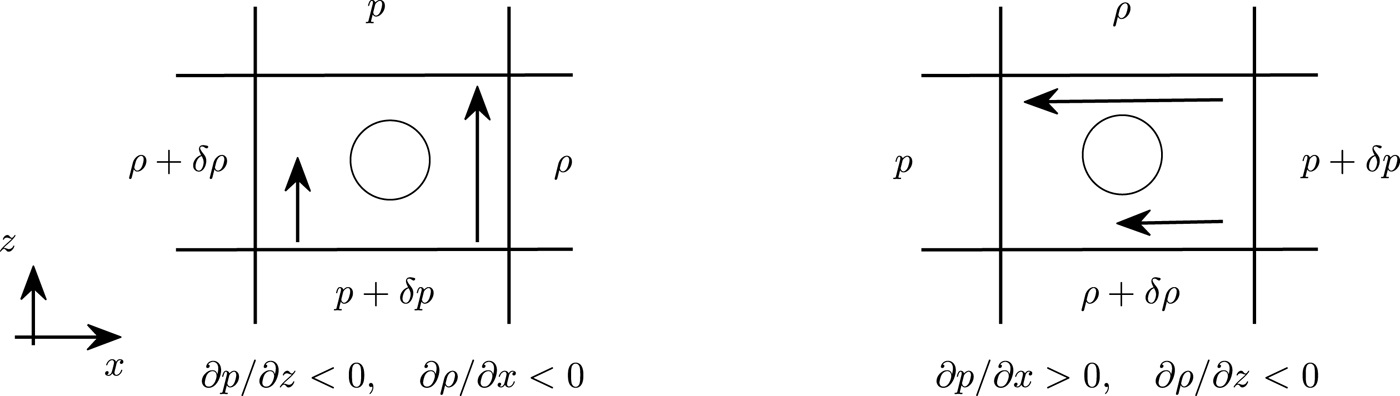
\includegraphics[width=0.9\textwidth]{./figs/intro_figs/baroclinic_schematic} \hfill
 \caption[A schematic of baroclinic torque]{From
    \cite{Heifetz2015}. A hydrostatic force balance upon a particle
    subject to perpendicular pressure and density gradients
    illustrates baroclinic torque on a fluid particle.}
  \label{fig:usbe_lung_baroclinic_schematic}
\end{figure}
Analytically, baroclinic vorticity generation can be shown by taking
the curl of the conservation of momentum equation for a compressible
fluid. It is worth noting that it is a nonlinear effect and cannot be
explained by traditional linear acoustics.

The physics of the classic \ac{RMI} are fairly well understood. For
the classical \ac{RMI} setup a planar shock impinges normally upon the
peaks and troughs of a sinusoidal interface. The interface is
accelerated non-uniformly counter-rotating vorticies are generated
across the interface. This drives peaks and troughs of the interface
to accelerate in the opposite direction. Much like in the case of the
\ac{RTI}, this too results in light fluid penetrating the
heavy fluid and vice versa. For the case of a wave moving from a light
fluid into a heavy one, the peaks and troughs of the interface
accelerate away from one another, growing the interface perturbation
perturbation. For the case of a wave moving from a heavy fluid to a
lighter fluid, the peaks and troughs interface initially accelerate
toward one another. They then pass each other, inverting the phase of
the interface perturbation, and continue moving in opposite
directions, growing the perturbation amplitude. This process is
illustrated in Figure \ref{fig:rmi_schematic}, which has been adapted
from \cite{Brouillette2002}. This work proposes that similar physics
occur at ultrasonically driven air-tissue interfaces within the lungs.
\begin{figure}
  \centering
  \def\svgwidth{0.9\textwidth}
  \import{./figs/intro_figs/}{brouillette_fig3_mod.pdf_tex} \hfill%
  \caption[A schematic view of the \acl{RMI} instability for a
  heavy-light interface]{Adapted from \cite{Brouillette2002}. The
    \ac{RMI} for a heavy-light interface is illustrated. The initial
    condition (left), circulation post wave-interface interaction
    (center), and perturbation growth (right) are shown.}
  \label{fig:rmi_schematic}
\end{figure}
 
\section{Thesis overview}
This part of the thesis presents work studying the physics of two
problems relevant to ultrasound bioeffects: 1) Cavitation of
ultrasound contrast agents microbubbles in human tissue, and 2)
\ac{DUS} of the lung. For each problem, a computational model is
developed and used to simulate the relevant dynamics in order to make
conclusions about the physics that may be relevant to the observed
biological effect.

In Chapter \ref{ch:usbe_bubble}, I simulate the cavitation bubble
dynamics of contrast agent microbubbles in soft tissue
\citep{Patterson2012}. Experimentally measured \ac{US} waves with
known bioeffects occurrence and thresholds are used
\cite{Miller2008b}.  A parametric study is performed, relating
ultrasound and tissue parameters to calculated cavitation bubble
dynamics. The soft tissue is modeled as a Voigt viscoelastic medium
based on the work of \cite{Yang2005}. The calculated cavitation
dynamics and theoretical inertial cavitation thresholds
\citep{Flynn1982,Apfel1982} are compared with bioeffects thresholds
associated with each \ac{US} pulse, as defined by the observation of
kidney hemorrhage in rats after exposure to CEUS by
\cite{Miller2008b}. While the results were generally dependent on
\ac{US}, gas, and tissue properties, it was found that the theoretical
inertial cavitation thresholds were lower than observed bioeffects
thresholds. It is shown that these thresholds correlate strongly to
calculated metrics of cavitation, such as dimensionless maximum radius
$R_{max}/R_{equilibrium}$ and that this correlation is lost when
simply looking at the dimensional maximum bubble size $R_{max}$, which
is not a cavitation metric.

In Chapter \ref{ch:usbe_lung}, I develop a model of an
ultrasonically-driven alveolus as a compressible, multi-phase fluid
system. This model is used to study the fundamental problem of an
acoustically-driven perturbed liquid-air interface. I demonstrate that
under the assumptions presented in Section \ref{sec:lung_assumptions},
strong acoustic waves of appropriate waveform are capable of
generating sufficient baroclinic vorticity to appreciably deform the
interface. The dependence of this deformation on the amplitude and
temporal characteristics of the wave is studied. It is demonstrated
that the deformation rate scales with the amount of circulation per
unit arc length of the interface. It is also shown that the amount of
circulation deposited by the wave is heavily dependent on the
deformation that occurs during the wave-interface interaction, and
therefore depends on the transient properties of the wave.

In Chapter \ref{ch:usbe_lung_bio}, the work of the previous chapter is
extended to increase its relevance to clinical \ac{US}. The model used
in the previous chapter is used to calculate the stresses and strains
induced by\ac{US} pulses on perturbed liquid-gas, similar to those of
the alveolus. These calculated stresses and strains are compared to
accepted failure criteria. It is shown that viscous stresses are small
compared to expected failure thresholds. However it is also shown that
strains at gas-liquid interfaces such as those of the lungs, driven by
acoustically-generated vorticity, may be sufficient to drive
hemorrhage for sufficiently strong ultrasound pulses. This work
concludes that while vorticity may be a possible mechanism for driving
\ac{DUS}-introduced lung hemorrhage, additional work will need to be
completed that accounts for multiple pulses as well as physical
effects of elasticity and viscosity in order fully understand the role
of vorticity in this problem.

In the final chapter \ref{ch:usbe_conclusions} of Part
\ref{part:ultrasound_bioeffects} of this dissertation, I summarize
the main conclusions takeaways and accomplishments of this work. I
Also make recommendations for future work to overcome the limitations
of the presented research and extend this work to address relevant
problems within the field.


% If the conservation  equations were kept separate
\begin{comment}
  \begin{align} \label{eq:intro_coma}
    \frac{\partial \rho}{\partial t} + \nabla\cdot\left(\rho\bs{u}\right) = 0,%
  \end{align}
  \begin{align} \label{eq:intro_como}% 
    \rho\frac{D \bs{u}}{D t} = \nabla\cdot\bs{\tau}+\bs{g},%
  \end{align}%
  \begin{align} \label{eq:intro_coe}%
    \frac{\partial}{\partial t}\left(\rho \left[e + \frac{\bs{u}\cdot\bs{u}}{2}\right]\right) + \nabla\cdot\left(\rho \left[e + \frac{\bs{u}\cdot\bs{u}}{2}\right]\bs{u}\right) = \rho\left(\bs{g}\cdot\bs{u}\right) + \nabla\cdot\left(\bs{\tau u}\right) + \nabla\cdot\bs{q}%
  \end{align}%
  \begin{align} \label{eq:stiffened_eos_intro}%
    E=\frac{\rho\left(u^2+v^2\right)}{2} + \frac{p+\gamma B}{\gamma-1}.
  \end{align}
\end{comment}


%%% Local Variables:
%%% mode: latex
%%% TeX-master: "../../main"
%%% End:

% The purpose of this introduction is to set the stage for the proposed
dissertation research. The problems we approach in this work are all
problems of interest, current to the field of Acoustics. Broadly,
acoustics is the study of sound. In practice, this study is not
limited to just the kinds of sound that can be heard by humans, but
rather any molecular scale vibrations traveling throughout a media. As
sounds both natural and man-made are ubiquitous, it is a topic that
has intrigued man for quite some time and attracted much attention and
study. As such, we have gained not only an understand the physical
nature of sound, but have also learned to harness it as a
tool. Because sound waves travel reflect, transmit, and scatter in a
mathematically describable way, they are ideally suited for gathering
information in certain situations. Because they carry mechanical
energy that can be focused, concentrated, and in some instances
converted into other types of energy, such as heat, they can also be a
powerful tool for physically altering an environment. In some
applications of interest, attempts to use acoustics to gather
information, can unintentionally lead to physical modification of the
system, such is the case when \ac{DUS} for medical imaging leads to
unintended biological effects, or ultrasound bioeffects as we will
refer to them from here on out.

Many problems of contemporary acoustic interest present challenges
that make them difficult to investigate completely through direct
experimentation. Some problems, such as certain ultrasound bioeffects,
often involve physical processes that occur over such small length and
time scales that they cannot be directly observed. When these
phenomena are replicated in simplified lab experiments, as they
frequently are, physical quantities of interest, like stress, are not
always readily measurable. Other problems may call for experiments
that are prohibitively costly and time-intensive, as is often the case
in underwater and ocean acoustics experiments which can require long
cruises with extensive personnel and equipment. Furthermore, in
complex acoustic environments like the ocean or human body, we rarely
have sufficient information to precisely and accurately describe the
system of interest without a high degree of uncertainty. In instances
such as these, where direct experimentation is infeasible or unable to
provide the desired information, carefully designed numerical
experiments can be useful for providing insight into the
problem at hand. 

The unifying theme of the work presented here is the use of
computation to approach modern problems in acoustics. The two main
areas of research considered are \acf{US} bioeffects and underwater
acoustic uncertainty. In the first part of this work, we investigate
two problems related to biological effects of medical
\ac{US}. Specifically, we simulate physics associated with \ac{CEUS}
and \ac{DUS} of the lung, which have both been shown to be capable of
causing hemorrhage in mammals, in order to investigate the damage
mechanism behind each. In the second part of this work we develop and
test area statistics, a computationally efficient method for
estimating the \ac{PDF} of acoustic \ac{TL} in uncertain ocean
environments, which is useful in naval applications. As these areas
are appreciably different, we will refer the reader to later portions
of this document and to the authors relevant submitted and published
works for more detailed introduction and background on each problem.

% %\subsection{\ac{US} background}
% Diagnostic \ac{US} has proven to be among the safest and most powerful
% medical imaging tools currently available and its use has become
% ubiquitous throughout modern medicine. The basic physical principle
% underlying this technology the scattering of sound at material
% interfaces. In practice, high-frequency, typically MHz range, acoustic
% waves and pulses are created at the surface of the body using a
% piezoelectric \ac{US} transducer. These vibrations propagate via an
% acoustic coupling medium from the transducer into the tissue and
% scatter whenever they encounter a change in the material properties of
% the medium. More simply, some of the sound echoes whenever it moves
% from one tissue to another, or hits a cavity in the body. These echoes
% are then picked up by a receiver and recorded. The strength and timing
% of these echoes allow for real-time imaging of the scattering surface.

% While clinical \ac{US} is generally incredibly safe there are
% specific instances during which \ac{US} can interact with tissue in
% such a way that it physically alters tissue. These effects to the body
% are referred to as \ac{US} bioeffects. While the entire field of
% therapeutic \ac{US} is based around intentionally causing
% bioeffects in a way that is beneficial to the patient, diagnostic
% \ac{US} is a different story. Bioeffects that occur during
% diagnostic \ac{US} typically take the form of unintended tissue
% damage or cell death. Depending on the type of physical damage
% mechanism responsible, these bioeffects are classified into two
% groups, thermal and non-thermal. The first group, thermal bioeffects
% are characterized by deposition of acoustic energy into tissue as
% heat. At the cellular and molecular scales, this can lead to the
% release of highly reactive free radicals, protein denaturation, and
% ultimately tissue damage and death. Little else will be said about
% thermal bioeffects, as the the bioeffects problems of interest to this
% work fall into the non-thermal category. The bulk of known non-thermal
% bioeffects are attributed to acoustically-induced cavitation.  

% Acoustic cavitation is the phenomenon by which gas nano and
% microbubbles, called cavitation nuclei, are cyclically grown by low
% pressures within the \ac{US} field and then collapsed high
% pressures within the field. When the bubble dynamics during collapse
% are dominated by the inertia of the surrounding fluid, it is called
% \ac{IC}. \ac{IC} is typically violent and results in the
% bubble collapsing to a fraction of its original size. There are
% several possible damage mechanisms associated with \ac{IC} that may be
% responsible for observed \ac{US} bioeffects. Upon collapse, the
% pressure and temperature within the bubbles spike, often reaching
% billions of pascals and thousands of Kelvin respectively. Due to the
% pressure difference between the vapor/gas mixture within the bubble at
% collapse and the surrounding media, the collapsed bubble can emit a
% powerful shock wave which can be damaging to the bubbles
% surroundings. When cavitation is triggered near a rigid surface, the
% bubble can collapse in a radially asymmetric fashion causing a high
% speed ``re-entrant'' jet of liquid to impinge upon the surface,
% effectively striking the surface with a liquid hammer \hl{CITE}. If
% cavitation occurs at an appropriate distance from a non-rigid surface,
% such as soft tissue boundaries and blood vessel walls, the jet can
% impinge away from the surface, potentially invaginating the surface
% \citep{Brujan2011}. \ac{CEUS}, which uses
% contrast-agent microbubbles injected into patients bloodstream to act
% as additional scattering surfaces. These microbubbles act as
% cavitation nuclei and have been associated with a variety of different
% forms of cellular death and damage.

% This proposal presents past work in which we simulate ultrasonically
% induced cavitation of contrast agent microbubbles in soft tissue
% \citep{Patterson2012} (See Chapter \ref{ch:usbe_bubble}).  We simulate
% experimentally measured \ac{US} waves obtained by \cite{Miller2008b}
% perturbing microbubbles in a Voigt viscoelastic soft tissue
% \cite[]{Yang2005}. The calculated cavitation dynamics and theoretical
% inertial cavitation thresholds \citep{Flynn1982,Apfel1982} are
% compared with bioeffects thresholds associated with each \ac{US}
% pulse, as defined by the observation of kidney hemorrhage in rats
% after exposure to CEUS by \cite{Miller2008b}. While the results were
% generally dependent on US, gas, and tissue properties, it was found
% that the inertial cavitation thresholds were lower than observed
% bioeffects thresholds.

% Another non-thermal \ac{US} bioeffect of interest is \ac{DUS}-induced
% \ac{LH}, which is the only known bioeffect of non-contrast \ac{DUS}
% known to occur in mammals. Despite the fact that this phenomenon was
% first observed in mice over twenty years ago \citep{Child1990}, the
% underlying physical damage mechanisms remain unknown. Research has
% shown that thermal damage mechanisms are unlikely as \ac{DUS}-induced
% lung lesions do not appear similar to those induced by heat
% \citep{Zachary2006}. Furthermore, cavitation mechanisms do not appear
% to be responsible, as the severity of \ac{DUS}-induced \ac{LH} in mice
% increased under raised hydrostatic pressure \citep{OBrien2000} and was
% unaffected by the introduction of \ac{US} contrast agents into
% subjects. Both of these results are inconsistent with what is expected
% of \ac{IC}-induced bioeffects. Works by \cite{Tjan2007,Tjan2008} model
% the evolution of an inviscid, free surface subjected to a Gaussian
% velocity potential and find that this can lead to the ejection of
% liquid droplets. They go on to say that \ac{DUS} of the lung may
% similarly lead to the ejected of droplets capable of puncturing the
% air-filled sacs within the lung. We propose another possible damage
% mechanism, that \ac{DUS} pulses torque tissue-air interfaces around
% alveoli, fragile air-sacs within the lungs. This deposits vorticity, a
% measure of local fluid rotation, in the surrounding fluid which drives
% deformation and ultimately hemorrhage of the thin alveolar walls.

% The concept of vorticity driven interface deformation has been
% extensively studied within the context of the \ac{RM}, which occurs
% when a traveling pressure wave, typically a shock, encounters a
% perturbed interface between fluids of different density. Note that the
% \ac{RM} is not a true instability, as the interface does not exhibit
% exponential growth. When this occurs vorticity is generated along the
% interface.

% As can be seen from the
% vorticity generation equation,
% \begin{align} \label{eq:vorticity}
% \frac{\partial \vec{\omega}}{\partial t}+\left(\vec{u}\cdot\nabla\right)\vec{\omega} = 
% \left(\vec{\omega\cdot\nabla}\right)\vec{u} - \vec{\omega}\left(\nabla\cdot\vec{u}\right)%
% +\frac{\nabla\rho\times\nabla p}{\rho^2} + \nabla\times\left(\frac{\nabla\cdot\tau}{\rho}\right)%
% +\nabla\times\left(\frac{\vec{B}}{\rho}\right)%
% \end{align}


% Computations of acoustic transmission loss are of practical interest in a variety of naval applications.






%%% Local Variables:
%%% mode: latex
%%% TeX-master: "../../main"
%%% End:

% \acresetall

% % US Bioeffects: 2012 Jasa Paper
\chapter{Theoretical microbubble dynamics at capillary breaching thresholds}   \label{ch:usbe_bubble}%
%\section{Abstract}
  In order to predict bioeffects in contrast-enhanced diagnostic and
  therapeutic ultrasound procedures, the dynamics of cavitation
  microbubbles in viscoelastic media must be determined.  For this
  theoretical study, measured 1.5-7.5 MHz pulse pressure waveforms,
  which were used in experimental determinations of capillary
  breaching thresholds for contrast-enhanced diagnostic ultrasound in
  rat kidney, were used to calculate cavitation nucleated from
  contrast agent microbubbles.  A numerical model for cavitation in
  tissue was developed based on the Keller-Miksis equation (a
  compressible extension of the Rayleigh-Plesset equation for
  spherical bubble dynamics), with a Kelvin-Voigt constitutive relation. From
  this model, the bubble dynamics corresponding to the experimentally
  obtained capillary breaching thresholds were determined. Values of
  the maximum radius and temperature corresponding to previously
  determined bioeffect thresholds were computed for a range of
  ultrasound pulses and bubble sizes for comparison to inertial
  cavitation threshold criteria.  The results were dependent on
  frequency, the gas contents, and the tissue elastic properties.  The
  bioeffects thresholds were above previously determined inertial
  cavitation thresholds, even for the tissue models, suggesting the
  possibility of a more complex dosimetry for capillary injury in
  tissue.


%%% Local Variables:
%%% mode: latex
%%% TeX-master: t
%%% End:

%In this chapter we present work in which experimentally-measured
\ac{US} pulses are used to simulate \ac{US} contrast agent microbubble
dynamics. The pulses were previously used in experiments to determine
capillary breaching thresholds in rat kidneys \citep{Miller2008b}. We
compare the calculated bubble dynamics to the
experimentally-determined bioeffects thresholds to investigate the use
of theoretical \ac{IC} thresholds as a predictor for bioeffects. This
work was published in the Journal of the Acoustical Society of America
\citep{Patterson2012, Patterson2012a}. Here we present the abstract, key figures, and
conclusions of the published work.
%
\section{Abstract}
  In order to predict bioeffects in contrast-enhanced diagnostic and
  therapeutic ultrasound procedures, the dynamics of cavitation
  microbubbles in viscoelastic media must be determined.  For this
  theoretical study, measured 1.5-7.5 MHz pulse pressure waveforms,
  which were used in experimental determinations of capillary
  breaching thresholds for contrast-enhanced diagnostic ultrasound in
  rat kidney, were used to calculate cavitation nucleated from
  contrast agent microbubbles.  A numerical model for cavitation in
  tissue was developed based on the Keller-Miksis equation (a
  compressible extension of the Rayleigh-Plesset equation for
  spherical bubble dynamics), with a Kelvin-Voigt constitutive relation. From
  this model, the bubble dynamics corresponding to the experimentally
  obtained capillary breaching thresholds were determined. Values of
  the maximum radius and temperature corresponding to previously
  determined bioeffect thresholds were computed for a range of
  ultrasound pulses and bubble sizes for comparison to inertial
  cavitation threshold criteria.  The results were dependent on
  frequency, the gas contents, and the tissue elastic properties.  The
  bioeffects thresholds were above previously determined inertial
  cavitation thresholds, even for the tissue models, suggesting the
  possibility of a more complex dosimetry for capillary injury in
  tissue.


%%% Local Variables:
%%% mode: latex
%%% TeX-master: t
%%% End:


\section{Key figures}
\label{sec:usbe_bubble_key_figures}
%\subsection{Bubble Response}
In this section we present key figures from \cite{Patterson2012a}. The
results presented are based on simulations of microbubbles in a Voigt
viscoelastic medium as modeled by \cite{Yang2005}. Experimentally
determined input pressure waveforms and the associated bioeffects are
based on the work performed in \cite{Miller2008b}.

To illustrate typical bubble responses, Figures
\ref{fig:sample_bubble_linear} and \ref{fig:sample_bubble_nonlinear}
show sample experimental input pressure waveforms from
\citep{Miller2008b} and the calculated bubble radius histories
corresponding to each. Both simulations are for the case of the wave
impinging upon an initially $R_0=1 \mu$m radius microbubble in Voigt
viscoelastic media with shear moduli, $G=5$ kPa, $100$ kPa, and $1$
MPa as indicated. Figure \ref{fig:sample_bubble_linear} represents an
essentially linear case with \ac{US} center frequency 1.5 MHz and 0.35
MPa \ac{PRPA}, in which no bioeffects were observed. Figure
\ref{fig:sample_bubble_nonlinear} represents a highly nonlinear case
with 7.5 MHz and 6.0 MPa \ac{PRPA}. In bioeffects, in the form of
bleeding on the surface of the rat kidney, were observed
\cite{Miller2008b}.
\begin{figure}%[h!]
  \centering
  \includegraphics[width=0.66\textwidth]{./figs/bubble_figs/rt_linear}
  \caption[Bubble radius history and input-pressure for an essentially linear case]{History of the bubble radius (top) and input-pressure
    waveform (bottom) for an essentially linear case (frequency: 1.5 MHz; \ac{PRPA}: 0.35 MPa). No bioeffects are observed
    here. $R_0=1$ $\mu$m; solid: $G=5$ kPa; dashed: $G=100$ kPa; dotted: $G=1$ MPa.}
  \label{fig:sample_bubble_linear}
\end{figure}
%
\begin{figure}%[h!]
  \centering \includegraphics[width=0.66\textwidth]{./figs/bubble_figs/rt_nonlinear}
  \caption[Bubble radius history and input-pressure for a nonlinear case]{History of the bubble radius (top) and input-pressure
    waveform (bottom) for a highly nonlinear case (frequency: 
    7.5 MHz; peak negative pressure: 6.0 MPa). Bioeffects are observed
    here. $R_0=1$ $\mu$m; solid: $G=5$ kPa; dashed: $G=100$ kPa; dotted: $G=1$ MPa.}
  \label{fig:sample_bubble_nonlinear}
\end{figure}

To study the dependence of the bubble dynamics on the gas content, we
compare results obtained for bubbles containing \ac{PFP} and air.
Figure \ref{fig:gascontents} shows sample bubble radii histories for
each gas and the corresponding input pressure wave. Additionally, we
plot of the maximum temperature for \ac{PFP} (circles) and air
(squares), calculated based on isentropic relationships, for bubbles
with initial radii $R_0=0.1-2$ $\mu$m exposed to ultrasound
frequencies 1.5 - 7.5 MHz and \ac{PRPA} 0.35 - 6 MPa.
\begin{figure*}%[h!]
  \includegraphics[width=0.47\textwidth]{./figs/bubble_figs/pfpair}% }
  \includegraphics[width=0.47\textwidth]{./figs/bubble_figs/tmaxpfpair}% }
  \caption[Dependence of the bubble dynamics on the gas contents]{ Dependence of the bubble dynamics on the gas contents ($G=100$ kPa). (Left) History of the bubble radius for \ac{PFP} (solid) 
    and air (dashed). (Right) Maximum temperature for \ac{PFP} (circles) and air (squares). $R_0=0.1-2$ $\mu$m; frequency: 1.5 - 7.5 MHz. }
  \label{fig:gascontents}
\end{figure*}

To illustrate the dependence of the bubble response on the pulse
frequency Figure \ref{fig:freq} shows the maximum dimensionless and
dimensional radius for all initial bubble sizes and amplitudes vs
frequency. The square symbols denote cases in which bioeffects were
observed in the experiments, while the circular symbols represent no
bioeffects. The initial bubble sizes are not discriminated here for
simplicity. With the exception of a few outliers, a clear separation
between cases for which bioeffects did and did not occur is observed;
in other words, the bioeffect threshold has a strong dependence on the
frequency. The trend appears to be approximately linear with
frequency. Large growth may be achieved with no evident bioeffects,
especially at high frequencies. The quantity $R_{max}$ is a measure of
cavitation collapse since it is related to the available energy of the
bubble. Thus, the present results indicate that cavitation collapse is
expected to play an important role regarding bioeffects, although the
precise mechanism cannot be inferred. Again, the existing criteria for
inertial cavitation thresholds are frequency-independent and do not
correlate well with the bioeffects threshold, which clearly shows a
strong dependence on frequency.
\begin{figure*}%[h!]
  \includegraphics[width=0.47\textwidth]{./figs/bubble_figs/rstarmax_f}  
  \includegraphics[width=0.47\textwidth]{./figs/bubble_figs/rmax_f}      
  \caption[Dependence of the bubble dynamics on the ultrasound frequency]{ Dependence of the bubble dynamics on the frequency for
    $G=100$ kPa. $R_0=0.1-2$ $\mu$m; empty circles: no bioeffects; squares:
    bioeffects. (Left) Dimensionless (Left) and dimensional (Right) maximum bubble radius.}
  \label{fig:freq}
\end{figure*}

To explore the effect of the elasticity on the results and the
correlation to bioeffects, Figure \ref{fig:freq_tissue} shows the
maximum dimensionless radius for all initial bubble sizes and
amplitudes vs frequency for $G=5$ kPa and $G=1$ MPa. Although
seemingly high, the latter elasticity is chosen to match the work of
\begin{figure*}%[h!]
  \includegraphics[width=0.47\textwidth]{./figs/bubble_figs/rstarmax_f_ca=20}
  \includegraphics[width=0.47\textwidth]{./figs/bubble_figs/rstarmax_f_ca=0,1}    
  \caption[Dependence of the dimensionless maximum bubble radius on
    the ultrasound frequency]{ Dependence of the dimensionless maximum bubble radius on
    the frequency for $G=5$ kPa (Left) and $G=1$ MPa (Right). $R_0=0.1-2$ $\mu$m; empty circles: no bioeffects; squares:
    bioeffects. }
  \label{fig:freq_tissue}
\end{figure*}

% \begin{figure*}[h!]
%   \subfigure[$G=5$ kPa.]{
%     \includegraphics[width=0.47\textwidth]{./figs/bubble_figs/rstarmax_f_ca=20}
%   }
%   \subfigure[$G=1$ MPa.]{
%     \includegraphics[width=0.47\textwidth]{./figs/bubble_figs/rstarmax_f_ca=0,1}    
%   }
%    \caption{ Dependence of the dimensionless maximum bubble radius on
%      the frequency. $R_0=0.1-2$ $\mu$m; empty circles: no bioeffects; squares:
%      bioeffects.}
%   \label{fig:freq_tissue}
% \end{figure*}
\clearpage
\pagebreak
\section{Conclusions}
\label{sec:conclusions}

In the present work, a numerical model is used
to investigate experimentally observed bioeffects as a result of
contrast-enhanced ultrasound. This work is unique in its 
combination of experimental results and numerical modeling.
For the experimentally generated input
pressure waveforms, it is known which of these triggered bioeffects,
and from the numerical model we obtained calculated values for
the dimensionless maximum radius and dimensional maximum temperature for each of these cases.  By comparing the
results of this study to previously established inertial cavitation
thresholds used by \cite{Apfel1991} and \cite{Yang2005},
$T_{max}=5000$ K and $R_{max}=2$, it would appear that the inertial
cavitation threshold does not play a role in determining the bioeffects
threshold.  However, it is unlikely that the inertial cavitation
threshold is irrelevant. Instead, it is far more probable that these
thresholds are not defined appropriately for cavitation in a
viscoelastic medium, such as soft tissue. This work suggests the need for
further experimental and numerical studies of cavitation in viscoelastic media.

The present work shows a strong correlation between cavitation dynamics and bioeffects
when considering the pulse frequency.
From the plot of maximum
dimensionless radius vs. frequency, there is a clear separation
between when bioeffects do and do not occur, and based on these
results it appears that the frequency of the input pressure waveforms
is of key importance to the definition of a bioeffect threshold, and
likely the inertial cavitation threshold as well. 

The present work shows that the elasticity of tissue significantly
affects the bubble dynamics. This finding is perhaps not completely
unexpected given that bubble dynamics are known to strongly depend
on viscoelastic properties and model. The present study shows the need
for more accurate measurements of material properties and for
determining appropriate constitutive models for soft tissue,
particularly at high strain rates. Finally, although the present work
suggests that inertial cavitation collapse plays an important role with respect
to bioeffects, it does not shed light on the exact mechanism,
\emph{e.g.}, shock emission upon collapse, growth beyond a given size,
high temperatures generating free radicals, re-entrant jets in
non-spherical collapse, etc.  In future work we plan on investigating 
this injury mechanism by conducting direct simulations of
the full equations of motion for bubble dynamics in a viscoelastic medium.


%%% Local Variables:
%%% mode: latex
%%% TeX-master: "../../prelim"
%%% End:


\begin{figure}
  \centering \includegraphics[width=0.66\textwidth]{./figs/bubble_figs/rt_linear}
  \caption{History of the bubble radius (top) and input-pressure
    waveform (bottom) for an essentially linear case (frequency: 1.5 MHz; peak y
    negative pressure: 0.35 MPa). No bioeffects are observed
    here. $R_0=1$ $\mu$m; solid: $G=5$ kPa; dashed: $G=100$ kPa; dotted: $G=1$ MPa.}
  \label{figure:sample_bubble_linear}
\end{figure}

\begin{figure}
  \centering 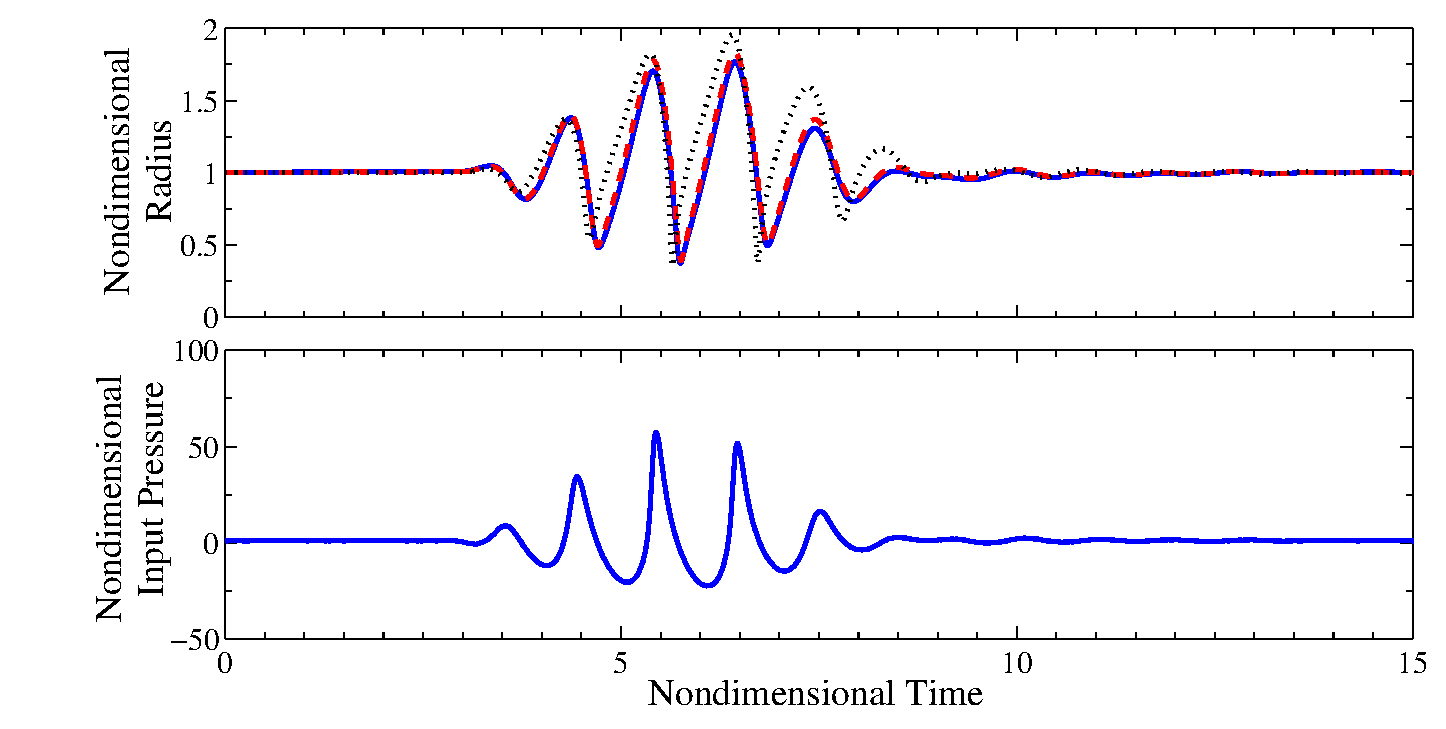
\includegraphics[width=0.66\textwidth]{./figs/bubble_figs/rt_intermediate}%
  \caption{History of the bubble radius (top) and input-pressure
    waveform (bottom) for a moderately nonlinear case (frequency: 3.5 MHz; peak 
    negative pressure: 2.4 MPa). Bioeffects are
    observed here. $R_0=1$ $\mu$m; solid: $G=5$ kPa; dashed: $G=100$ kPa;
    dotted: $G=1$ MPa.}
  \label{figure:sample_bubble_intermediate}
\end{figure}

\begin{figure}
  \centering \includegraphics[width=0.66\textwidth]{./figs/bubble_figs/rt_nonlinear}
  \caption{History of the bubble radius (top) and input-pressure
    waveform (bottom) for a highly nonlinear case (frequency: 
    7.5 MHz; peak negative pressure: 6.0 MPa). Bioeffects are observed
    here. $R_0=1$ $\mu$m; solid: $G=5$ kPa; dashed: $G=100$ kPa; dotted: $G=1$ MPa.}
  \label{figure:sample_bubble_nonlinear}
\end{figure}

In the results of the following sections, the maximum dimensionless radius,
$R_{max}$, and dimensional bubble temperature at collapse, $T_{max}$, obtained
using the ideal gas law, are determined by recording their largest
value over the simulation. These quantities are compared to the
inertial cavitation thresholds used by \cite{Apfel1991} and
\cite{Yang2005}: $R_{max}=2$ and $T_{max}=5000$ K. The dependence
of the bubble dynamics on the pulse amplitude, initial
bubble size (\emph{i.e.}, UCA size distribution), 
pulse frequency, and tissue properties are considered
individually. 



\subsection{Dependence on the Pulse Amplitude}

Given the strong dependence of the MI on the rarefactional pressure
amplitude, the influence of the pulse amplitude on the bubble dynamics
is first evaluated. Fig.~\ref{figure:amplitude} shows the dimensionless
maximum radius as a function of rarefactional pressure
amplitude. Initial bubble radii ranging between 0.1--2.0 $\mu$m are
shown, as well as different frequencies. The open symbols denote
cases where bioeffects did not occur, while the filled symbols denote
the occurrence of bioeffects.

\begin{figure}[t]
  \includegraphics[width=\columnwidth]{./figs/bubble_figs/rstarmax_pm}
  \caption{(color online) Dependence of the dimensionless maximum bubble radius on
    the peak negative pressure for $G=100$ kPa.  Empty symbols: no
    bioeffects; filled symbols: bioeffects. Pentagrams: 0.1 $\mu$m; circles:
    0.5 $\mu$m; squares: 1 $\mu$m; diamonds: 2 $\mu$m; frequency: 1.5 - 7.5 MHz. }
  \label{figure:amplitude}
\end{figure}

The results show that the bubble dynamics, through the maximum radius,
scale with the pulse amplitude. Although the results do not collapse fully
onto a line, a general trend is discernible. At low amplitude, the increase in
the maximum radius is approximately linear; beyond some amplitude, the bubble undergoes
nonlinear oscillations, thus explaining the different depenced and larger spread. 
These results are consistent with the plots shown in 
Figs.~\ref{figure:sample_bubble_linear}-\ref{figure:sample_bubble_nonlinear}.
Over a broad range of amplitudes, the
occurrence of bioeffects has little correlation with pulse amplitude
alone: at a given amplitude, bioeffects may be observed or not,
depending on the bubble size and pulse frequency.  Only at very large
pressure amplitudes (PRPA $>$ 4.20 MPa) are bioeffects systematically observed regardless of the
bubble size and pulse frequency. This behavior is not surprising, since at
these amplitudes the bubble response is expected to be highly
nonlinear. Conversely, at low amplitudes (PRPA $<$ 0.97 MPa), the oscillations are 
linear and no bioeffects are observed, regardless of
bubble size and pulse frequency. In this latter case, most bubbles
whose $R_{max}/R_o$ is below two do not exhibit bioeffects; however,
this behavior depends on the value of elasticity, as shown in \S
\ref{section:tissue_properties}.  Although not shown here for conciseness,
similar results are obtained for peak positive pressure.


Similarly, the criterion $T_{max} > 5000$ K is not achieved with perfluoropropane.
As shown in Fig.~\ref{figure:gascontents}, the observed temperatures for
PFP are far below this value, though the results for air approach it. This
result is expected since the criterion was determined for air, which
has a larger specific heats ratio ($\gamma_{air}=1.4$) than
PFP ($\gamma= 1.13$). The specific heats ratio appears in
the internal gas pressure term in Eq.~\ref{eq:bubble_pressure}; its
effect on the bubble dynamics is minor if the minimum radius is not
very small, as in Fig.~\ref{figure:gascontents}. Still, since the
adiabatic relationships for an ideal gas are used, the temperature is
significantly affected by the different specific heats ratio. Hence,
even though the bubble dynamics are not strongly affected by the
specific heats ratio, the maximum temperature is.

\begin{figure*}[t]
  \begin{subfigure}[b]{0.47\textwidth}
  \includegraphics[width=\textwidth]{./figs/bubble_figs/pfpair}
  \caption{History of the bubble radius for PFP (solid) and air
    (dashed). $R_0=1$ $\mu$m; frequency: 3.5 MHz; peak negative
    pressure: 3.3 MPa}
\end{subfigure}
  \begin{subfigure}[b]{0.47\textwidth}
    \includegraphics[width=\textwidth]{./figs/bubble_figs/tmaxpfpair} 
    \caption{Maximum temperature for PFP (circles) and air (squares). $R_0=0.1-2$ $\mu$m; frequency: 1.5 - 7.5 MHz.}
  \end{subfigure}
  \caption{(color online) Dependence of the bubble dynamics on the gas contents ($G=100$ kPa).}
  \label{figure:gascontents}
\end{figure*}

% \begin{figure*}[t]
%   \subfigure[History of the bubble radius for PFP (solid) 
%     and air (dashed). $R_0=1$ $\mu$m; frequency: 3.5 MHz; peak negative pressure: 3.3 MPa]{
%   \includegraphics[width=0.47\textwidth]{./figs/bubble_figs/pfpair} }
%   \subfigure[Maximum temperature for PFP (circles) and air (squares). $R_0=0.1-2$ $\mu$m; frequency: 1.5 - 7.5 MHz. ]{
%   \includegraphics[width=0.47\textwidth]{./figs/bubble_figs/tmaxpfpair} }
%   \caption{(color online) Dependence of the bubble dynamics on the gas contents
%   ($G=100$ kPa).}
%   \label{figure:gascontents}
% \end{figure*}






\subsection{Dependence on the Initial (Equilibrium) Bubble Radius}

In the experiment, the size distribution of the UCAs is not known
exactly. It is desirable to know whether the observed bioeffects are
caused by all bubbles responding to the ultrasound, or whether a
specific size is more likely to be responsible at the bioeffects
threshold. To answer this question, for each experimental frequency,
bubbles of different radii ranging from 0.1--2 $\mu$m are subjected to
the pressure waveform corresponding to the bioeffects threshold
amplitude. It should be noted that varying the equilibrium radius
changes the non-dimensional parameters. Fig.~\ref{figure:size} shows the maximum dimensionless
radius, for both water (zero elasticity) and tissue (finite
elasticity, $G=100$ kPa), for the amplitude at which bioeffects are
first observed at a given frequency.

\begin{figure}[t]
    \includegraphics[width=\columnwidth]{./figs/bubble_figs/rstarmax_r0}
    \caption{(color online) Dependence of the dimensionless maximum bubble radius on
      the initial bubble size for the amplitude at which bioeffects
      are first observed, at a given frequency, for $G=100$ kPa. Empty
      symbols: water; filled symbols: tissue. Circles: 1.50 MHz; squares:
      2.25 MHz; diamonds: 3.50 MHz; pentagrams: 5.00 MHz; hexagrams: 7.50 MHz.}
    \label{figure:size}
\end{figure}

Excluding the smallest size, the bubble response in tissue is monotone
and changes little for a given frequency; there is no initial size
that consistently leads to a dramatic response. The somewhat erratic
behavior of the small bubbles may imply that such sizes are not
present in UCA concentrations. On the other hand, the behavior is more
irregular for water, particularly at small radii: for a given
frequency, there is an optimal size that exhibits the largest
response; these variations are much larger than for tissue.  








\subsection{Dependence on the Pulse Frequency}

The dependence of the bubble response on the pulse frequency is
considered in this section.  Fig.~\ref{figure:freq} shows the maximum
dimensionless and dimensional radius for all initial bubble sizes and
amplitudes vs. frequency. The square symbols denote cases in which
bioeffects were observed in the experiments, while the circular symbols
represent no bioeffects. The initial bubble sizes are not
discriminated here for simplicity.


\begin{figure*}[t]
  \begin{subfigure}[b]{0.47\textwidth}
    \includegraphics[width=\textwidth]{./figs/bubble_figs/rstarmax_f}  
    \caption{Dimensionless maximum bubble radius.}
  \end{subfigure}

  \begin{subfigure}[b]{0.47\textwidth}
    \includegraphics[width=0.47\textwidth]{./figs/bubble_figs/rmax_f}      
    \caption{Dimensional maximum bubble radius.}
  \end{subfigure}
  \caption{(color online) Dependence of the bubble dynamics on the frequency for
    $G=100$ kPa. $R_0=0.1-2$ $\mu$m; empty circles: no bioeffects; squares:
    bioeffects.}
  \label{figure:freq}
\end{figure*}

With the exception of a few outliers, a clear separation between cases
for which bioeffects did and did not occur is observed; in other
words, the bioeffects threshold has a strong dependence on the
frequency. The trend appears to be approximately linear with
frequency. Large growth may be achieved with no evident bioeffects,
especially at high frequencies. The quantity $R_{max}$ is a
measure of cavitation collapse, since it is related to the available
energy of the bubble. Thus, the present results indicate that
cavitation collapse is expected to play an important role regarding
bioeffects, although the precise mechanism cannot be inferred.  Again,
the existing criteria for inertial cavitation thresholds are
frequency-independent and do not correlate well with the bioeffects
threshold, which clearly shows a strong dependence on frequency.

Another hypothesis is that bubble growth may be responsible for
capillary breaching. However, the plot of the dimensional maximum radius vs. frequency does
not show systematic bioeffects beyond a certain size, \emph{e.g.},
some capillary diameter. Thus, growth is not the sole mechanism by
which bioeffects occur. However, the data remains inconclusive,
due to the inability to identify the cases in which cavitation
collapse is the dominant effect.






\subsection{Dependence on the Tissue Properties}
\label{section:tissue_properties}

As suggested in
Figs.~\ref{figure:sample_bubble_linear}-\ref{figure:sample_bubble_nonlinear},
the bubble dynamics are sensitive to the tissue properties,
specifically the elasticity. However, different types of tissue may
have very different properties. Many of the measurements of tissue elasticity are made
\emph{in vitro}, and depend strongly on tissue preparation, storage,
and degradation as well as method of measurement.  Consequently it is
possible that these measurements do not accurately represent the
current behavior.  To explore the effect of the elasticity on the
results and the correlation to bioeffects, Fig.~\ref{figure:freq_tissue}
shows the maximum dimensionless radius for all initial bubble sizes
and amplitudes vs. frequency for $G=5$ kPa and $G=1$ MPa. Although
seemingly high, the latter elasticity is chosen to match the work of
\cite{Yang2005}.

\begin{figure*}[t]
  \begin{subfigure}[b]{0.47\textwidth}
    \includegraphics[width=\textwidth]{./figs/bubble_figs/rstarmax_f_ca=20}
    \caption{$G=5$ kPa.}
  \end{subfigure}

  \begin{subfigure}[b]{0.47\textwidth}
    \includegraphics[width=\textwidth]{./figs/bubble_figs/rstarmax_f_ca=0,1}    
    \caption{$G=1$ MPa.}
  \end{subfigure}
  \caption{(color online) Dependence of the dimensionless maximum bubble radius on
     the frequency. $R_0=0.1-2$ $\mu$m; empty circles: no bioeffects; squares:
     bioeffects.}
  \label{figure:freq_tissue}
\end{figure*}

% \begin{figure*}[t]
%   \subfigure[$G=5$ kPa.]{
%     \includegraphics[width=0.47\textwidth]{./figs/bubble_figs/rstarmax_f_ca=20}
%   }
%   \subfigure[$G=1$ MPa.]{
%     \includegraphics[width=0.47\textwidth]{./figs/bubble_figs/rstarmax_f_ca=0,1}    
%   }
%    \caption{(color online) Dependence of the dimensionless maximum bubble radius on
%      the frequency. $R_0=0.1-2$ $\mu$m; empty circles: no bioeffects; squares:
%      bioeffects.}
%   \label{figure:freq_tissue}
% \end{figure*}

The bubble dynamics and correlation to bioeffects significantly change
when reducing the elasticity. For a value of 5 kPa, the discrimination
is no longer clear. The bubble dynamics are closer to the behavior in
water, such that different sizes may have dramatically different
responses to the same waveform, as explained previously. On the other
hand, the stiffer medium ($G=1$ MPa) shows an even sharper
demarcation, which again appears to be approximately linear. Given the
sensitivity of the results on the elasticity, it is clear that more
precise \emph{in vivo} data is required for elasticities of tissues at the
relevant strain rates. 

Although not shown here, the type of
viscoelastic model significantly affects the bubble dynamics
\cite[]{Johnsen2012}. For instance, a standard linear solid
model, which includes stress relaxation in addition to elasticity, leads 
to very different maximum
radii and oscillation properties (frequency and damping).  For
large relaxation times, elasticity variations become negligible.




\section{Conclusions}
\label{sec:usbe_bubble_conclusions}

In the present work, a numerical model is used
to investigate experimentally observed bioeffects as a result of
contrast-enhanced ultrasound. This work is unique in its 
combination of experimental results and numerical modeling.
For the experimentally generated input
pressure waveforms, it is known which of these triggered bioeffects,
and from the numerical model we obtained calculated values for
the dimensionless maximum radius and dimensional maximum temperature for each of these cases.  By comparing the
results of this study to previously established inertial cavitation
thresholds used by \cite{Apfel1991} and \cite{Yang2005},
$T_{max}=5000$ K and $R_{max}=2$, it would appear that the inertial
cavitation threshold does not play a role in determining the bioeffects
threshold.  However, it is unlikely that the inertial cavitation
threshold is irrelevant. Instead, it is far more probable that these
thresholds are not defined appropriately for cavitation in a
viscoelastic medium, such as soft tissue. This work suggests the need for
further experimental and numerical studies of cavitation in viscoelastic media.

The present work shows a strong correlation between cavitation dynamics and bioeffects
when considering the pulse frequency.
From the plot of maximum
dimensionless radius vs. frequency, there is a clear separation
between when bioeffects do and do not occur, and based on these
results it appears that the frequency of the input pressure waveforms
is of key importance to the definition of a bioeffect threshold, and
likely the inertial cavitation threshold as well. 

The present work shows that the elasticity of tissue significantly
affects the bubble dynamics. This finding is perhaps not completely
unexpected given that bubble dynamics are known to strongly depend
on viscoelastic properties and model. The present study shows the need
for more accurate measurements of material properties and for
determining appropriate constitutive models for soft tissue,
particularly at high strain rates. Finally, although the present work
suggests that inertial cavitation collapse plays an important role with respect
to bioeffects, it does not shed light on the exact mechanism,
\emph{e.g.}, shock emission upon collapse, growth beyond a given size,
high temperatures generating free radicals, re-entrant jets in
non-spherical collapse, etc.  In future work we plan on investigating 
this injury mechanism by conducting direct simulations of
the full equations of motion for bubble dynamics in a viscoelastic medium.


%%% Local Variables:
%%% mode: latex
%%% TeX-master: t
%%% End:

\acresetall
% %
% Acoustically-driven gas-liquid interfaces


% US Bioeffects: DUS-induced Lung Hehorrage work
\chapter{Growth of liquid-gas interfacial perturbations driven by acoustic waves} \label{ch:usbe_lung}%
\input{./content/chapters/usbe_lung_paper_chapter}


\acresetall
\chapter{Pulsed ultrasound-induced stresses and strains at gas-liquid interfaces} \label{ch:usbe_lung_bio}%
In the Chapter \ref{ch:usbe_lung} we introduced the problem of
\ac{DUS}-induced lung hemorrhage, however the focus was on the
fundamental physical problem of an acoustically driven gas-liquid
interface, such as those of the alveoli. In this chapter we aim to
extend that work to increase its relevance to \ac{DUS} of the
lung. Here, I hypothesize that \ac{DUS} may be capable of generating
sufficient baroclinic vorticity at alveolar interfaces in the lung to
drive deformation and hemorrhage. To investigate this hypothesis I
examine the dynamics of water-air interfaces driven by ultrasound
pulses and compute relevant stresses and strains at the interface for
comparison to expected damage thresholds based on previous research.

\section{Introduction}
Lung \ac{US} has become a common tool for imaging and diagnostics in
critical and point-of-care situations and its use is growing
\citep{Lichtenstein2009}. Currently, \ac{PH} is the only biological
effect known to occur in mammals as a result of non-contrast
diagnostic ultrasound and it has been shown to occur under clinically
acceptable parameters with \ac{MI}$\leq1.9$ \citep{FDA1997} and peak
pressures as low as $1$ MPa \citep{Dalecki1997}. The physical
mechanism underlying this damage is still not well understood. And
while the occurrence of hemorrhage as a result of diagnostic lung
\ac{US} has not been directly studied in human lungs for obvious
ethical reasons, an understanding of the underlying cause is important
for the development of safe guidelines and procedures.

In Chapter \ref{ch:usbe_lung}, the body of literature covering
research into the physical mechanisms of \ac{DUS} was reviewed, so
only a brief summary will be provided here. Pulmonary damage induced
by pulsed ultrasound is characterized by hemorrhage of plasma proteins
and erythrocytes into the alveoli \cite{Penney1993a}. Alveolar edema
or frank hemorrhage has also been shown to occur as a result of
mechanical stress failure of the alveolar membrane induced by over
pressure \citep{West1991}. \ac{DUS}-induced hemorrhage in the lungs
appears mechanical in nature and thermal mechanisms appear unlikely
\citep{Zachary2006, Dalecki2004}. Among possible mechanical damage
mechanisms cavitation, acoustic radiation force, acoustic fountaining
or atomization have all been considered. Experimental results suggest
that neither inertial cavitation nor radiation force can completely
explain the damage \citep{OBrien2000, Raeman1996, Miller2016}. This
work aims to use numerical experiments to investigate the stresses and
strains imparted by an ultrasound pulse on a perturbed liquid-gas
interface, such similar to those of the alveoli.

The anatomical structure of the lungs has been studied extensively and
is of particular interest to the present work. The alveoli can be
thought of as a network of openly connected, air-filled saccules with
distinctly irregular surfaces. And while alveoli are irregularly
shaped and do not have a true diameter, past research suggests that
their size appears to be species dependent \citep{Faffe2002}. Mean
alveolar diameters range from tens to hundreds of microns with
reported values of 45 $\mu$m in mice \cite{Knust2008} and 200 $\mu$m
in adult humans \cite{Ochs2004} for examples. The septa that separate
adjacent alveoli are nearly planar structures that contain several
tissue layers and are coated with a thin layer of liquid surfactant
\citep{Gil1979,Reifenrath1975,Perlman2014}. Among the tissue layers
surrounding the alveoli is a sheet-like web of blood-filled
capillaries. These pulmonary capillaries are almost completely
unsupported by surrounding tissue \cite{West1991}. Separating the
blood from the air is a multi-layer wall of tissues, $0.2$ - $0.3\mu$m
thick, referred to as the blood-gas or \ac{BAB} \citep{West2000}. The
extreme thinness of this barrier is necessary for efficient gas
exchange. The physical dimensions of the alveolus and thinness of this
barrier relative to typical \ac{US} wavelengths are of importance to
the model used in this study.

In addition to anatomical structure, the mechanical properties and
failure behavior of alveoli and other relevant pulmonary tissues have
been studied extensively in computational and animal
models. \cite{Perlman2014} combined experimentally measured strains
with computationally modeled lung stresses to demonstrate that the
effective Young's moduli of aveolar septa depend on transpulmonary
pressure. Values range from $E_a=12$ kPa at a low transpulmonary
pressure around $0.4$ kPa to $E_a=140$ kPa at a high transpulmonary
pressure of approximately $2$ kPa. \cite{West1991} raised the
pulmonary capillary pressure of anesthetized rabbits and observed
consistent stress failure of the capillary and alveolar epithelium for
transmural at or above $40$ mmHg ($5.3$ kPa). This failure
corresponded to a $\sim25$ mN/m wall tension in the capillaries, which
is ``comparable with the tension in the alveolar wall''. The capillary
wall stress at failure was calculated to be approximately $8$
kPa. \begin{comment}
  This is roughly consistent with \cite{Welling1972} which measured
  properties of basement membranes from rabbit renal tubules and
  showed that a $57 \mu$m tubule could withstand $4.1$ kPa transmural
  pressure, which, based on a Laplace relationship, equates to an
  ultimate tensile strength of 500 kPa \citep{West1999}. Furthermore,
  \cite{Welling1972} also showed that properties of these tubules
  depended only on the strength of their basement membrane.
\end{comment}

Alveolar strain response has also been previously studied. Linear,
alveolar strain due to normal tidal breathing is in the range of
$0$-$5$\% \citep{Roan2011}. And \cite{Vlahakis2000} reports that
alveolar plasma membranes resist lateral tension and fail under
stresses greater than $0.4-0.6$ Pa, which corresponds to strains of
$2-3\%$. However, this work also acknowledges that typical changes in
cellular surface area are primarily a result of plasma membrane
unfolding and not actual wall strain. \citep{Belete2010} found that
when subjected to cyclical linear stretch at 0.5 Hz for 30 minutes,
rat alveolar epithelial cells experiencing Linear strains of $8\%$ or
greater were frequently damaged, whereas those experiencing strains
of $3 - 6\%$ often undamaged. 

Based on the work the previous chapter and the past research of
alveolar stress and strain failure we investigate the role of pulsed
ultrasound in possible stress and strain failure of alveoli. In this
chapter numerical experiments to simulate the dynamics of gas-liquid
interfaces driven by ultrasound pulse waveforms within the clinically
relevant range. Specifically, based on the work of Chapter
\ref{ch:usbe_lung}, I look for vorticity driven strains of the
interface, and establish simple models for computing the associated
passive viscous and elastic stresses. The computed stresses and
strains are compared to established failure criteria for alveoli to
access the relevance of this work to \ac{DUS} induced lung hemorrhage.


%%%%%%%%%%%%%%%%%%%%%%%%%%%%%%% 
\section{Methods}
Much of the basic problem setup, computational framework, and solution
setup laid out in Chapter \ref{ch:usbe_lung} are used here. In this
section I will focus specifically on three specific areas where
changes have been made to increase the relevance of the problem to
diagnostic ultrasound: (1) Problem geometry, (2) The acoustic wave,
(3) The calculation of stress and strain.

\subsection{Problem geometry}
In the previous section, we simulated trapezoidal acoustic waves
impinging upon a nearly planar interface with a sinusoidal
perturbation. The width of the domain represents a signle alveolar
diameter, $\ell$. The amplitude $a_0$ of this pertubation was $0.03\%$
its wavelength, again $\ell$, and for the sake of our simulation
corresponds $3\%$ the diameter of an alveolus. This implies a nearly
flat alveolar surface, which as we can see is not always the case,
based on the histological cross section of alveoli shown in Figure
\ref{fig:alveolar_histology}. To account for the variety of geometries
in alveolar tissue, many of which are not particularly flat, I will
now also consider perturbation amplitudes of $a_0=0.1\ell$ and
$a_0=0.3\ell$. I note that this in no way accounts for the range of
cross-sectional alveolar geometries that can exist, but we are limited
by computational constraints and our ability to resolve small scale
features that appear for larger perturbations and sharper geometries.
\begin{figure}
  \centering
  \begin{subfigure}[b]{0.45\textwidth}
    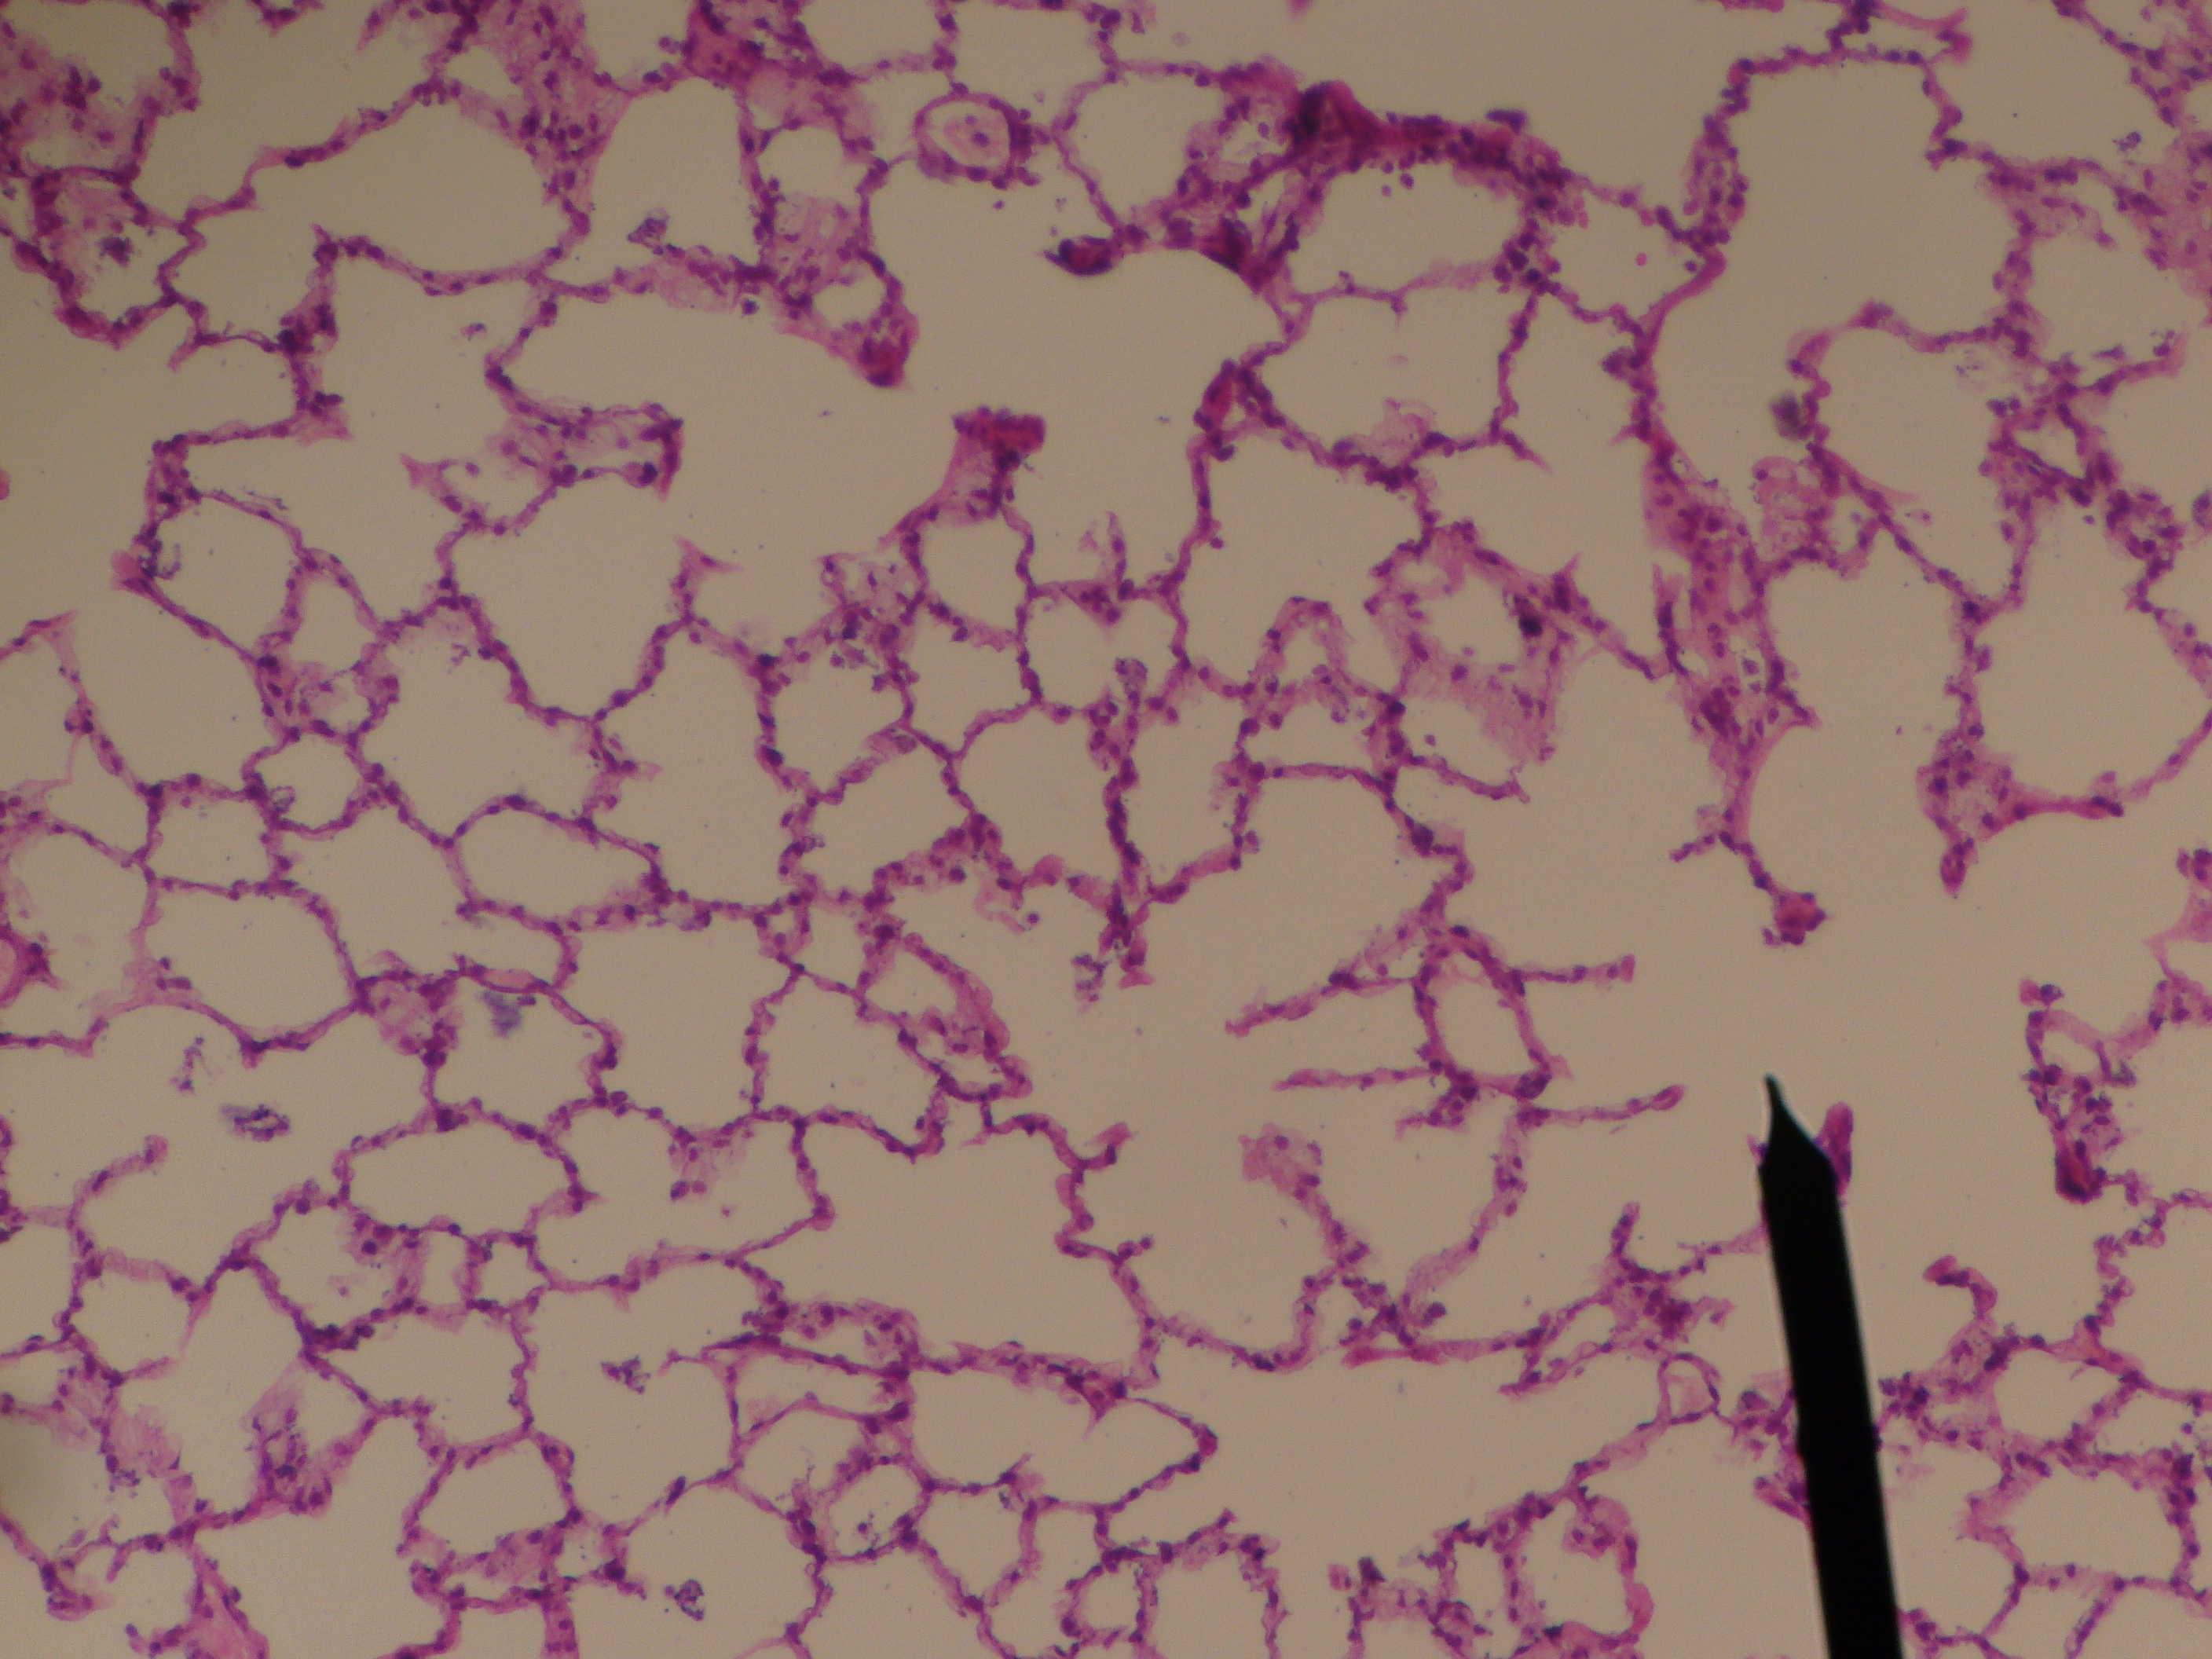
\includegraphics[width=\textwidth]{./figs/lung_figs/alveolar_sac}
    \caption{\label{fig:alveolar_histology}A histological cross section of alveoli. [By Jpogi (Own work) [CC BY-SA 4.0
      (http://creativecommons.org/licenses/by-sa/4.0)], via Wikimedia
      Commons]}
  \end{subfigure}
  % ~
  % \begin{subfigure}[b]{0.45\textwidth}
  %   \centering
  %   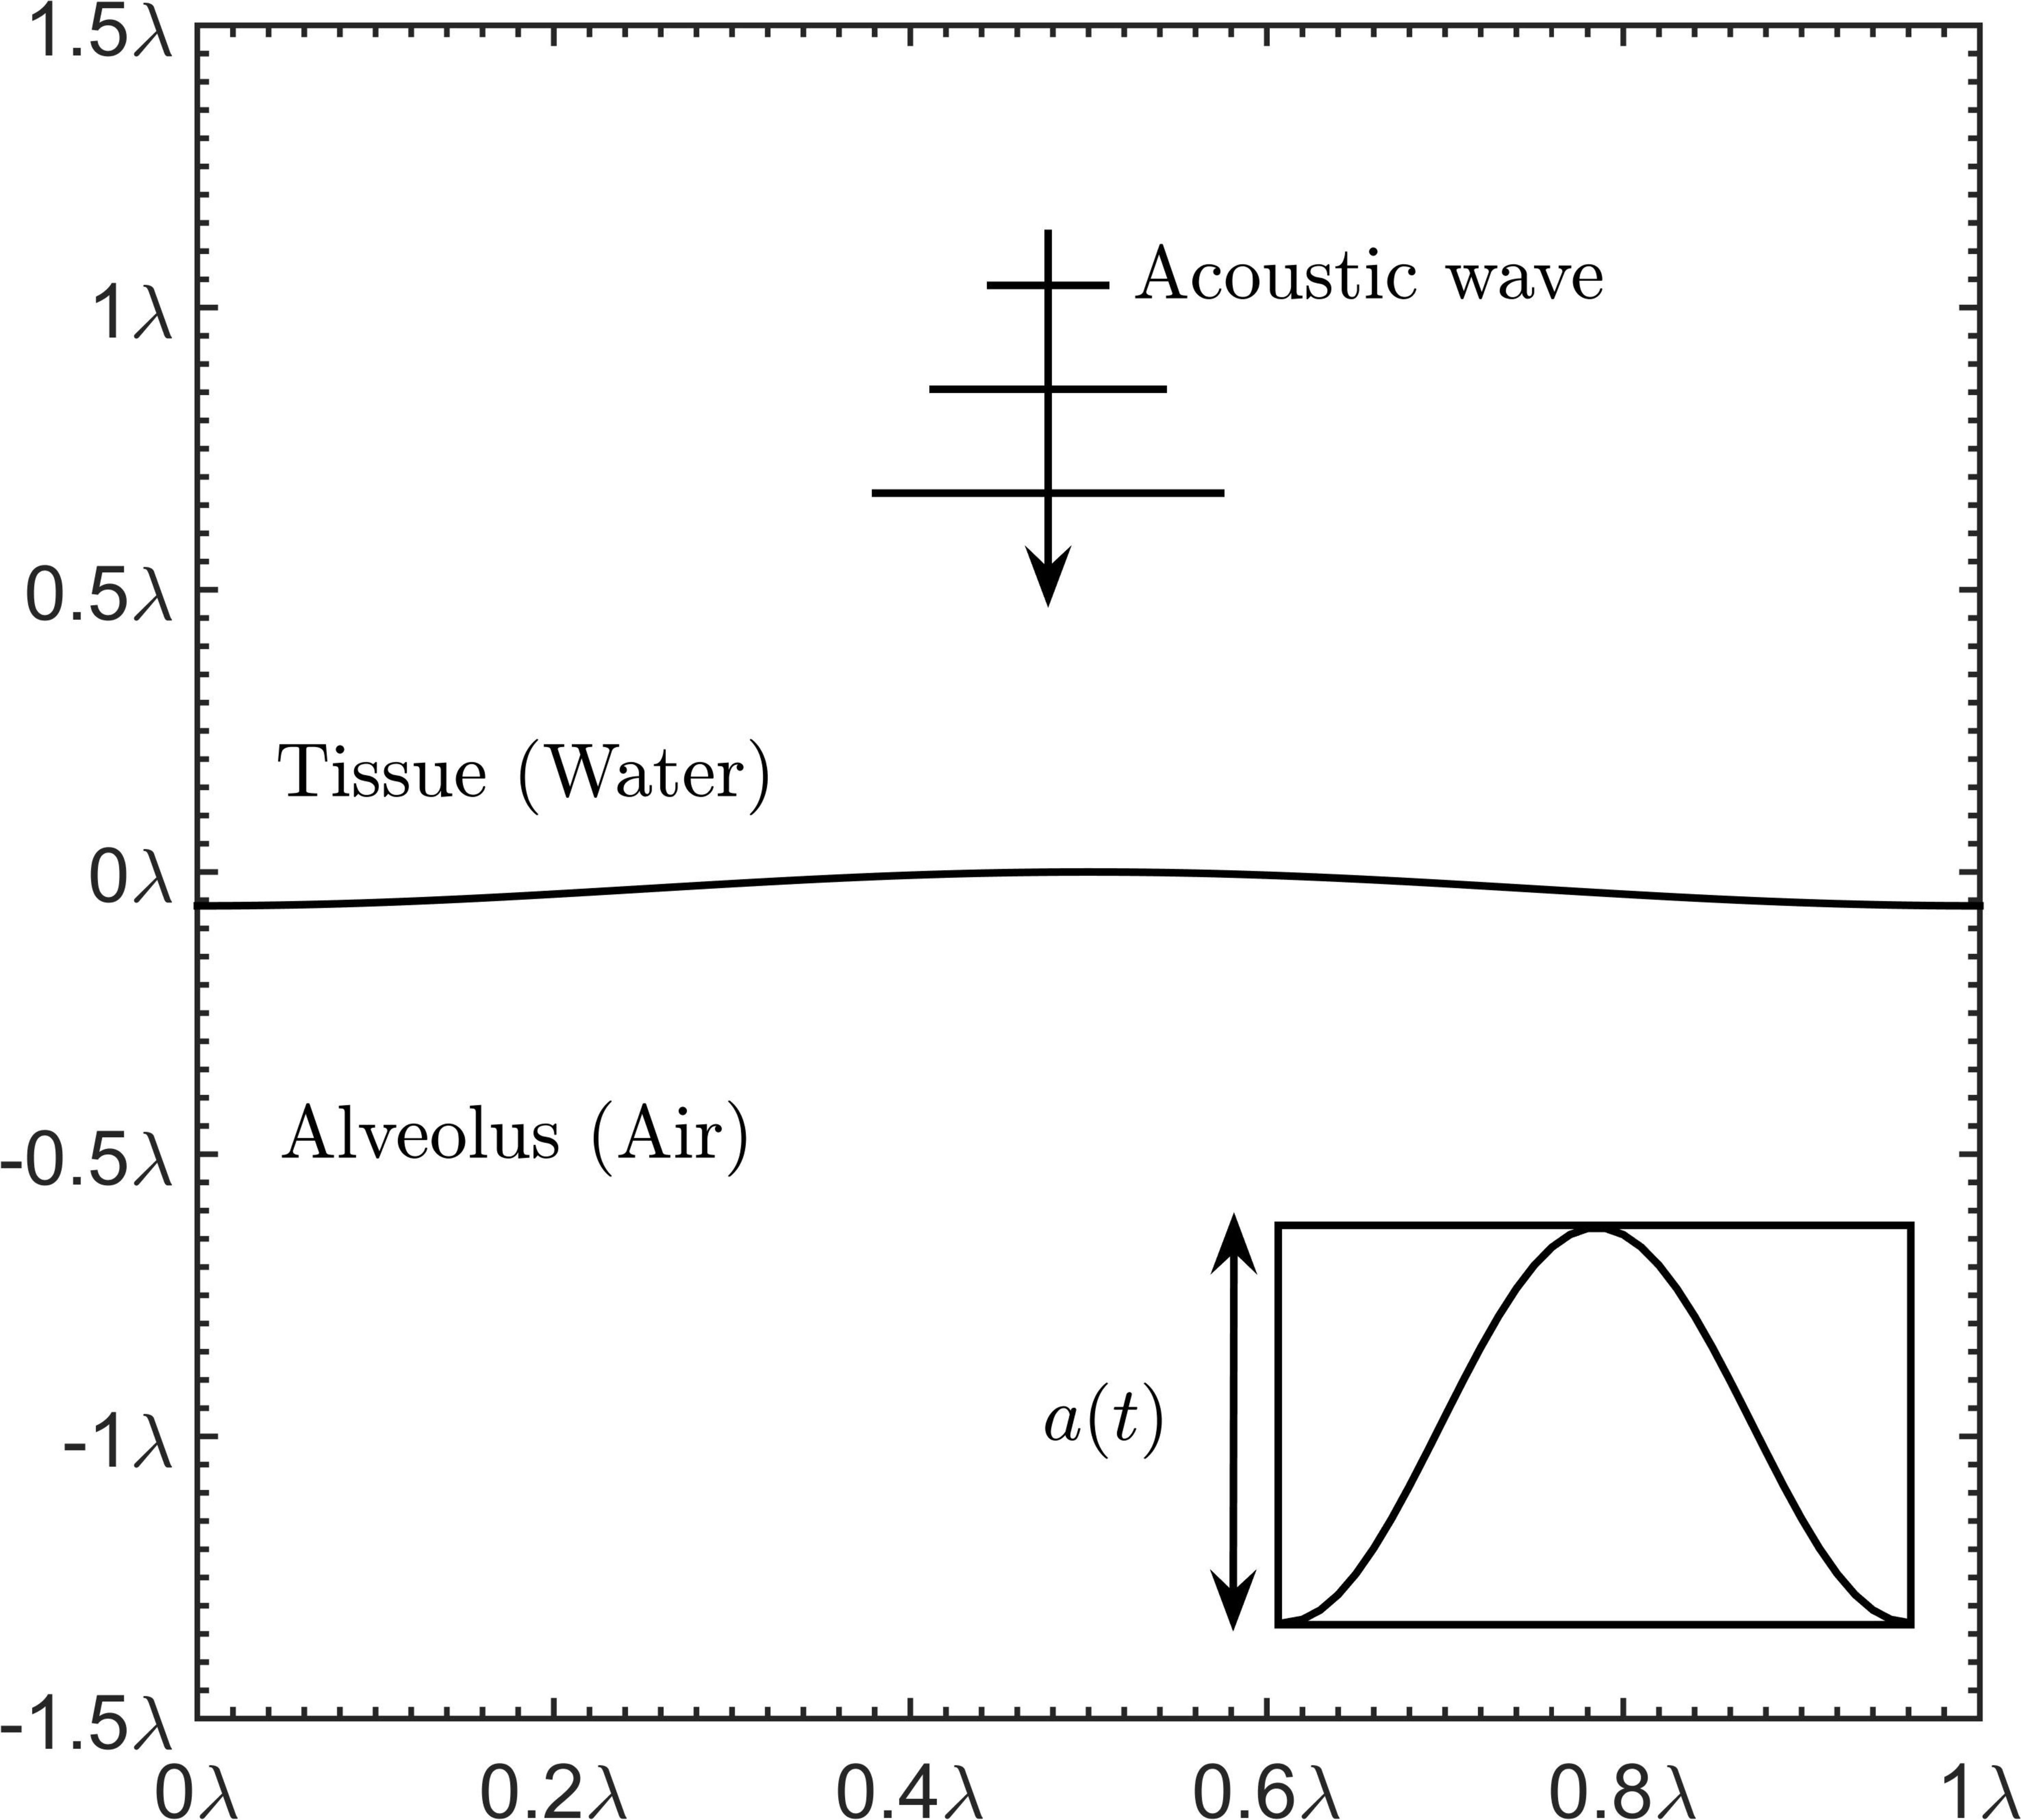
\includegraphics[width=\textwidth]{./figs/lung_figs/problem_schematic}
  %   \caption{\label{fig:ic_schematic}\hl{(STILL TO BE MODIFIED)}A
  %   schematic view of the model problem.}
  % \end{subfigure}
  \caption{A cross sectional view of alveolar tissue \protect\subref{fig:alveolar_histology}}
\end{figure}
% 
\subsection{Modeling the diagnostic ultrasound pulse}
The diagnostic ultrasound pulse is modeled as a sinusoidal carrier
wave of amplitude $p_a$ and frequency $f$ modulated by a Gaussian
Envelope such that,
\begin{align}
  p(x,t_0) = p_a\sin{\left(2\pi f\frac{\left[y-\left(Y_{wave}+L_{wave}\right)\right]}{c}\right)}\exp{\left(-\frac{\left(\left[y-\left(Y_{wave}+L_{wave}/2\right)\right]c\right)^2}{FWHM/\left(2\sqrt{2\ln{\left(2\right)}} \right)}\right)}.%
\end{align}
\begin{figure}
  \centering
%  \begin{subfigure}[b]{0.45\textwidth}
    \def\svgwidth{0.5\textwidth}
    \import{./figs/lung_figs/}{p0_vs_t_us_general.pdf_tex}%
%    \includegraphics[width=\textwidth]{./figs/lung_figs/}
    \caption{\label{fig:alveolar_histology} Sample ultrasound pulse waveform}
%  \end{subfigure}
\end{figure}

The carrier wavelength $\lambda=c_{water}/f$ and the full width of the
Gaussian envelope at half of the maximum amplitude ($FWHM$) are
designed to scale appropriately with respect to $\ell$. Here, we
choose design parameters of $f\approx 1.25 c_{water} / 2\pi \ell$ and
$FWHM=15\ell$ such that for an alveolar length scale of
$\ell=200 \mu$m, the corresponding center frequency is $f=1.65$ MHz
and $FWHM=3$ mm. $L_{wave}=45\ell$ is the length of the portion of the
computational domain, over which the wave is defined to exist, such
that the approximate duration of the wave-interface interaction is
just under $6 \mu$s. $Y_{wave}$ is $y$-location of the bottom of the
wave at $t=0$, which is set to $10a_0$ above the peak of the
interface. To consider the dependence of the interface dynamics on
pulse amplitude within the relevant range we vary $p_a = 1, 2.5,$ and
$5$ MPa.

\subsection{Stress and strain at the alveolar interface}%
\label{subsec:usbe_lung_bio_stress_strain}
To interpret the results of the numerical experiments to be performed
in the context of \ac{DUS}-induced lung injury, we aim to compare to
accepted stress and strain injury criteria for lung tissue. To do this
we calculate the strain of the air-water interface and the passive
viscous stress in the field. We note that from the available strain
and strain rate data, it would be possible to compute a passive total
viscoelastic stress at the interface if an acceptable constitutive
model were available. However, constitutive models appropriate to this
work do not appear available at this time and the development of such is beyond the scope of
this dissertation. For sake of justification of the model, a simple
model for estimating the order of magnitude of the involved elastic
forces can be found in \ref{app:lung_elastic}

\paragraph*{Calculation of the viscous stress}
We aim to calculate an approximate viscous stress, however because we
solve the Euler equations our simulations are inherently of an
inviscid flow. We do this because, while the justifications in Chapter
\ref{ch:usbe_lung} suggest that flow dynamics can be reasonably
approximated by neglecting viscosity, to understand the results in the
context of alveolar injury, an understanding of the approximate
viscous stress associated with \ac{DUS} is essential. To do this, we
calculate a passive viscosity at each point in space and time as
$\mu(x,y,t)$ based on the physical properties of air and water, and
the volume fraction of water $\alpha(x,y,t)$ such that
$\mu = \alpha\mu_{water} + (1-\alpha)\mu_{air}$. The shear stress for
a two-dimensional, Newtonian flow is calculated using the computed
viscosity field and the velocity gradients as
\begin{align}
  \tau_{xy}(x,y,t) = \mu\left(\frac{du}{dy}+ \frac{dv}{dx}\right).
\end{align}
The maximum viscous stress is extracted from the field. As will be
shown, this maximum occurs as the interface and as such, it will be
compared to relevant stress failure criteria.
%
\begin{comment}
  \begin{align}%
    \tau_{ij}=\mu%
    \begin{bmatrix}%
      0 & \frac{du}{dy}+\frac{dv}{dx}\\%
      \frac{dv}{dx}+\frac{du}{dy} & 0%
    \end{bmatrix}%
  \end{align},
\end{comment}
%
\paragraph*{Calculation of the interface strain}
The interface strain is calculated as 
\begin{align}%
  \label{eq:linear_strain}%
  \varepsilon = \frac{s(t) - s_0}{s_0}
\end{align}
where $s$ is the arc length of the interface.  This is consistent with
previous alveolar strain calculations by \cite{Roan2011}, which used
the relative change in alveolar diameters, which is analagous to the
interface arc length here.

%%%%%%%%%%%%%%%%%%%%%%%%%%%%%%% 
\section{Results and Discussion}
Simulations of interactions between sinusoidally perturbed water-air
interfaces and diagnostic ultrasound pulses were performed for wave
amplitudes of $p_a=1$, $2.5$, and $5$ MPa and initial perturbation
amplitudes of $a_0=0.03\ell$, $0.1\ell$ and $0.3\ell$.

\subsection{Qualitative observations of the interface}
Figures \ref{fig:rho_snapshots_A10}, \ref{fig:rho_snapshots_A25}, and
\ref{fig:rho_snapshots_A50} show density contour snapshots of the
interface for pulse amplitudes of $1, 2.5,$ and $5$ MPa respectively
at dimensionless times $t=1, 10, 100,$ and $500$. In each case,
subfigures \subref{fig:rho_snapshot_03}, \subref{fig:rho_snapshot_10},
and \subref{fig:rho_snapshot_30} correspond to initial perturbation
amplitudes of $a_0=0.03\ell, 0.1\ell,$ and $0.3\ell$ respectively. For
a $200 \mu$m, alveolar diameter, these times approximately corresponds
to $t^*=0.6, 6, 60,$ and $300 \mu$s. $t=1$ occurs just after the wave
first encounters the interface and $t=10$ is approximately when it has
completely passed the interface. For the $p_a = 1$ MPa pulse case seen
in Figure \ref{fig:rho_snapshots_A10}, the interface remains largely
unmoved and undeformed by the interaction with the wave, even at late
time. For the $p_a = 2.5$ MPa pulse case, little deformation is
observed for $a_0 = 0.03\ell$, however at higher initial amplitudes
$a_0 = 0.1\ell$ and $0.3\ell$, the interface is clearly deformed and
cusp is observed to form at the interface peak $x = 0.5$ at late
times. For the $p_a = 5$ MPa pulse obvious deformation is observed for
every $a_0$. For $a_0 = 0.1\ell$ and $0.3\ell$ and a spike of heavy
fluid with a cusp at $x = 0.5$ is again observed to form at late
times.  For all incoming waves, the degree of deformation appears to
increase with increasing initial perturbation amplitude $a_0$ and wave
amplitude $p_a$. The observed sharp features, which evolved from an
initially smooth interface perturbation, could potentially lead to
stress concentration which in aveoli, may lead to hemorrhage.
%
\begin{figure}
  \vspace*{-0.5cm}
  \centering
  \begin{subfigure}[b]{0.9\textwidth}
    \includegraphics[width=\textwidth]{./figs/lung_figs/rmawave_1_A10_a03_t500_rho_snapshots}
    \caption{\label{fig:rho_snapshot_03} $a_0 = 0.03\ell$}
  \end{subfigure}
  % 
  \begin{subfigure}[b]{0.9\textwidth}
    \includegraphics[width=\textwidth]{./figs/lung_figs/rmawave_1_A10_a10_t500_rho_snapshots}
    \caption{\label{fig:rho_snapshot_10} $a_0 = 0.1\ell$}
  \end{subfigure}
  % 
  \begin{subfigure}[b]{0.9\textwidth}
    \includegraphics[width=\textwidth]{./figs/lung_figs/rmawave_1_A10_a30_t500_rho_snapshots}
    \caption{\label{fig:rho_snapshot_30} $a_0 = 0.3\ell$}
  \end{subfigure}
  
  \caption{Density contours are plotted to show the evolution of the interface at $t=0, 10, 100,$
    and $500$ for initial perturbation amplitude $a_0 = 0.03\ell$ and wave amplitude $p_a=1$ MPa.}
  \label{fig:rho_snapshots_A10}
\end{figure}
%
%
\begin{figure}
  \vspace*{-0.5cm}
  \centering
  \begin{subfigure}[b]{0.9\textwidth}
    \includegraphics[width=\textwidth]{./figs/lung_figs/rmawave_1_A25_a03_t500_rho_snapshots}
    \caption{\label{fig:rho_snapshot_03} $a_0 = 0.03\ell$}
  \end{subfigure}
  % 
  \begin{subfigure}[b]{0.9\textwidth}
    \includegraphics[width=\textwidth]{./figs/lung_figs/rmawave_1_A25_a10_t500_rho_snapshots}
    \caption{\label{fig:rho_snapshot_10} $a_0 = 0.1\ell$}
  \end{subfigure}
  % 
  \begin{subfigure}[b]{0.9\textwidth}
    \includegraphics[width=\textwidth]{./figs/lung_figs/rmawave_1_A25_a30_t500_rho_snapshots}
    \caption{\label{fig:rho_snapshot_30} $a_0 = 0.3\ell$}
  \end{subfigure}
  % 
  \caption{The evolution of the interface is shown for $t=0, 10, 100,$
    and $500$ for varying initial perturbation amplitudes and a wave amplitude of $p_a=2.5$ Pa.}
  \label{fig:rho_snapshots_A25}
\end{figure}
%
\begin{figure}
  \vspace*{-0.5cm}
  \centering
  \begin{subfigure}[b]{0.9\textwidth}
    \includegraphics[width=\textwidth]{./figs/lung_figs/rmawave_1_A50_a03_t500_rho_snapshots}
    \caption{\label{fig:rho_snapshot_A50_a03} $a_0 = 0.03\ell$}
  \end{subfigure}
  % 
  \begin{subfigure}[b]{0.9\textwidth}
    \includegraphics[width=\textwidth]{./figs/lung_figs/rmawave_1_A50_a10_t500_rho_snapshots}
    \caption{\label{fig:rho_snapshot_A50_a10} $a_0 = 0.1\ell$}
  \end{subfigure}
  % 
  \begin{subfigure}[b]{0.9\textwidth}
    \includegraphics[width=\textwidth]{./figs/lung_figs/rmawave_1_A50_a30_t500_rho_snapshots}
    \caption{\label{fig:rho_snapshot_A50_a30} $a_0 = 0.3\ell$}
  \end{subfigure}
  % 
  \caption{The evolution of the interface is shown for $t=0, 10, 100,$
    and $500$ for varying initial perturbation amplitudes and a wave amplitude of $p_a=5$ Pa.}
  \label{fig:rho_snapshots_A50}
\end{figure}
%
%
\subsection{Ultrasound-induced Vorticity generation}
And in Chapter \ref{ch:usbe_lung} it was demonstrated that interface
deformations that occurred following acoustic waves were indeed driven
by baroclinic vorticity. And, at the beginning of this chapter, I
hypothesized that ultrasound waves may also be capable of generating
baroclinic vorticity at alveolar interfaces within the lungs, capable
of inducing strains which may partially account for some of the lung
hemorrhage observed as a result of \ac{DUS}. Thus far, results have
been presented demonstrating appreciable ultrasound induced
deformation of the interface. I now aim to investigate if vorticity is
also the like cause of deformations observed as a result of the
ultrasound wave.

Figure \ref{fig:us_vorticity_snapshots} illustrates the vorticity
field at $t=1, 10, 100, and 500$ for $p_a = 2.5$
\ref{fig:vorticity_snapshot_A25_a03} and $5$ MPa
\ref{fig:vorticity_snapshot_A50_a03} for $a_0 = 0.03\ell$. The $1$ MPa
case is excluded because little deformation was observed over the
simulated period. $a_0 = 0.03\ell$ is chosen, as this is the case in
which the least baroclinic vorticity expected because of greater
alignment between the ultrasound pressure and interface density
gradients. 
%
\hl{BETTER SNAPSHOTS}
\begin{figure}
  \centering
  \begin{subfigure}[b]{0.9\textwidth}
    \begin{tikzpicture}%
      \node[anchor=south west,inner sep=0] (image) at (0,0) {
        \includegraphics[width=\textwidth]{./figs/lung_figs/rmawave_1_A25_a03_t500_vorticity_snapshots}
      };%
      \begin{scope}[x={(image.south east)},y={(image.north west)}]%
        \node[font=\normalsize,right] at (0.07,0.13) {$t=1$};%
        \node[font=\normalsize,right] at (0.28,0.13) {$t=10$};%
        \node[font=\normalsize,right] at (0.5,0.13) {$t=100$};%
        \node[font=\normalsize,right] at (0.73,0.13) {$t=500$};%
      \end{scope}%  
    \end{tikzpicture}%
    \caption{\label{fig:vorticity_snapshot_A25_a03} $p_a = 2.5$ MPa, $a_0 = 0.03\ell$}
  \end{subfigure}
  %
  \begin{subfigure}[b]{0.9\textwidth}
    \begin{tikzpicture}%
      \node[anchor=south west,inner sep=0] (image) at (0,0) {
        \includegraphics[width=\textwidth]{./figs/lung_figs/rmawave_1_A50_a30_t500_vorticity_snapshots}
      };%
      \begin{scope}[x={(image.south east)},y={(image.north west)}]%
        \node[font=\normalsize,right] at (0.07,0.13) {$t=1$};%
        \node[font=\normalsize,right] at (0.28,0.13) {$t=10$};%
        \node[font=\normalsize,right] at (0.5,0.13) {$t=100$};%
        \node[font=\normalsize,right] at (0.73,0.13) {$t=500$};%
      \end{scope}%  
    \end{tikzpicture}%
    \caption{\label{fig:vorticity_snapshot_A50_a30} $p_a = 5$ MPa, $a_0 = 0.3\ell$}
  \end{subfigure}
  \caption{Snapshots of the vorticity field at $t=1, 10, 100,$ and
    $500$ are shown for two example cases. Figure
    \subref{fig:vorticity_snapshot_A25_a03} shows the vorticity
    fields for the case for which very little late time deformation
    occurs, in which $p_a = 2.5$ MPa, $a_0 = 0.03\ell$. Figure
    \subref{fig:vorticity_snapshot_A50_a30} shows the vorticity
    fields for the case for which there is significant late late-time
    deformation of the interface, in which $p_a = 5$ MPa,
    $a_0 = 0.3\ell$.}
  \label{fig:us_vorticity_snapshots}
\end{figure}
%
To obtain a cumulative measure of vorticity deposited by the
ultrasound wave we integrate the vorticity field at each point in time
over the right-half domain to obtain the circulation, $\Gamma$. We
note that by symmetry the circulation in the left half of the domain
is equal an opposite such that the total circulation over the
computational domain is zero.

To illustrate the dependence of the ultrasound-generated circulation
on $a_0$, Figure \ref{fig:us_circulation_a0_dependence} shows the
circulation history $\Gamma(t)$ for the $p_a = 5$ MPa case for
$a_0 = 0.03\ell$ (blue), $0.1\ell$ (red) and $0.3\ell$ (green). During
the wave-interface interaction ($t \leq 10$), the circulation
fluctuates rapidly as subsequent pressure fluctuations deposit
vorticity of opposite sign. During this period there appears to be a
complicated relationship between circulation and $a_0$. However, after
the passage of the wave the amount of circulation remaining appears to
increase with increasing $a_0$. Small fluctuations in the circulation
after the passage of the wave are a result of numerical reflections
within the domain.

To illustrate the dependence of the ultrasound-generated circulation
on $p_a$, Figure \ref{fig:us_circulation_a0_dependence} shows the
circulation history $\Gamma(t)$ for the $a_0 = 0.3\ell$ case for
$a_0 = 0.03\ell$ (blue), $0.1\ell$ (red), and $0.3\ell$
(green). During the wave-interface interaction $t \leq 10$, the
circulation again fluctuates rapidly, however it can be seen that the
chronologically local mean circulation increases with increasing $p_a$
as would be expected since the amplitude of the pressure gradient also
rises. After the passage of the wave the amount of circulation
remaining increases with increasing $p_a$, though not necessarily
according to a purely linear relationship.

After the passage of the \ac{US} pulse, there are no obvious
mechanisms, besides remaining baroclinic vorticity, to drive the
continued deformation of the interface. As such, it is worth
discussing what precisely contributes to the circulation remaining
after the passage of the wave. Throughout the wave-interface
interaction, the interface itself deforms such that while \ac{US}
pressure gradient is continuously misaligned with portions of the
interface density gradient, the degree to that misalignment changes in
time. While this deformation appears to be nominally small based on
the density snapshots provided in Figures \ref{fig:rho_snapshots_A03},
\ref{fig:rho_snapshots_A25}, \ref{fig:rho_snapshots_A50}, it is
measurable and critical to the vorticity dynamics. Because the
pressure returns to ambient after the passage of the wave, it must be
true that the integral of the acoustic pressure gradient over all time
is zero. Thus the only way that baroclinic vorticity can remain after
the passage of the wave is though changes in the density gradient. As
the interface deforms the direction these small changes in the
direction and local magnitude of the density gradient result in a net
deposition of circulation that remains to deform the interface after
the passage of the wave. This has particular relevance to ultrasound
which relies on many subsequent pulses, potentially resulting in the
accumulation of vorticity over time.
\begin{figure}
  \centering
  \begin{subfigure}[b]{0.49\textwidth}
    \begin{tikzpicture}%
      \node[anchor=south west,inner sep=0] (image) at (0,0) {
        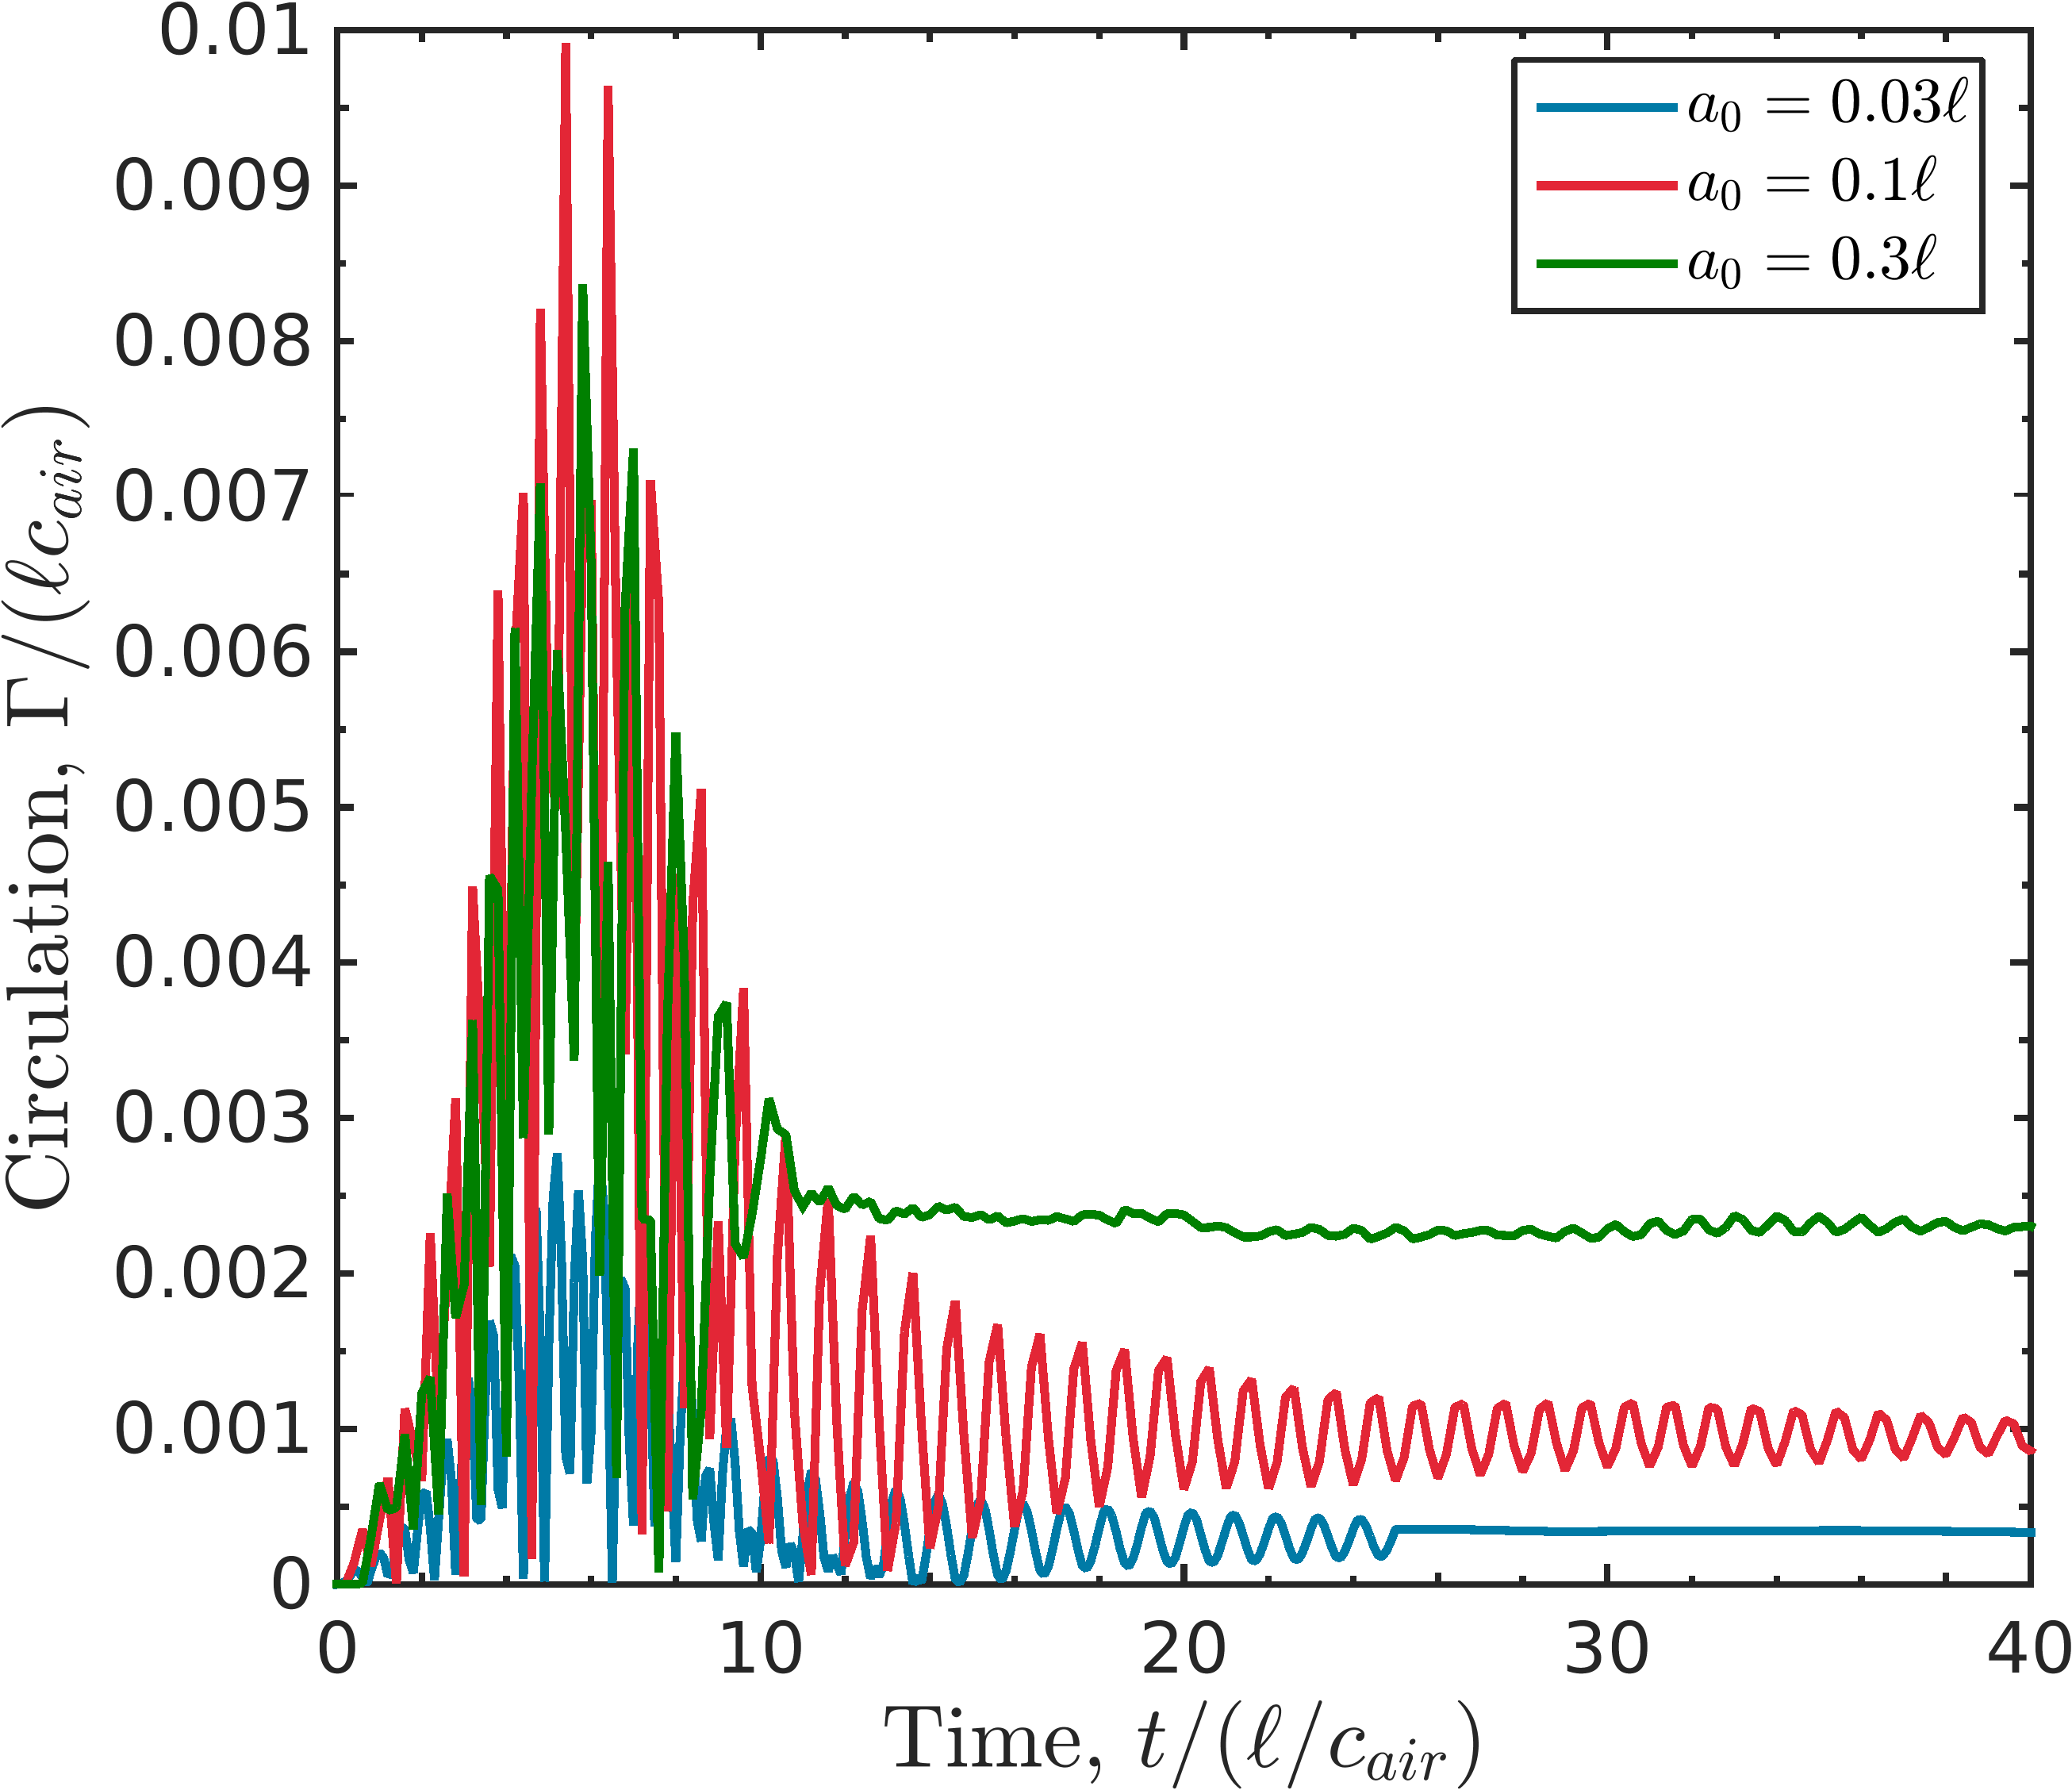
\includegraphics[width=\textwidth]{./figs/lung_figs/rmawave_1_A50_a03,10,30_circulation_01-Mar-2017}
      };%
      \begin{scope}[x={(image.south east)},y={(image.north west)}]%
        \node[font=\normalsize,right] at (0.07,0.13) {};%
      \end{scope}%  
    \end{tikzpicture}%
    \caption{\label{fig:us_circulation_a0_dependence} $p_a = 5$ MPa, $a_0 = 0.03\ell, 0.1\ell, 0.3\ell$}
  \end{subfigure}
  ~
  \begin{subfigure}[b]{0.49\textwidth}
    \begin{tikzpicture}%
      \node[anchor=south west,inner sep=0] (image) at (0,0) {
        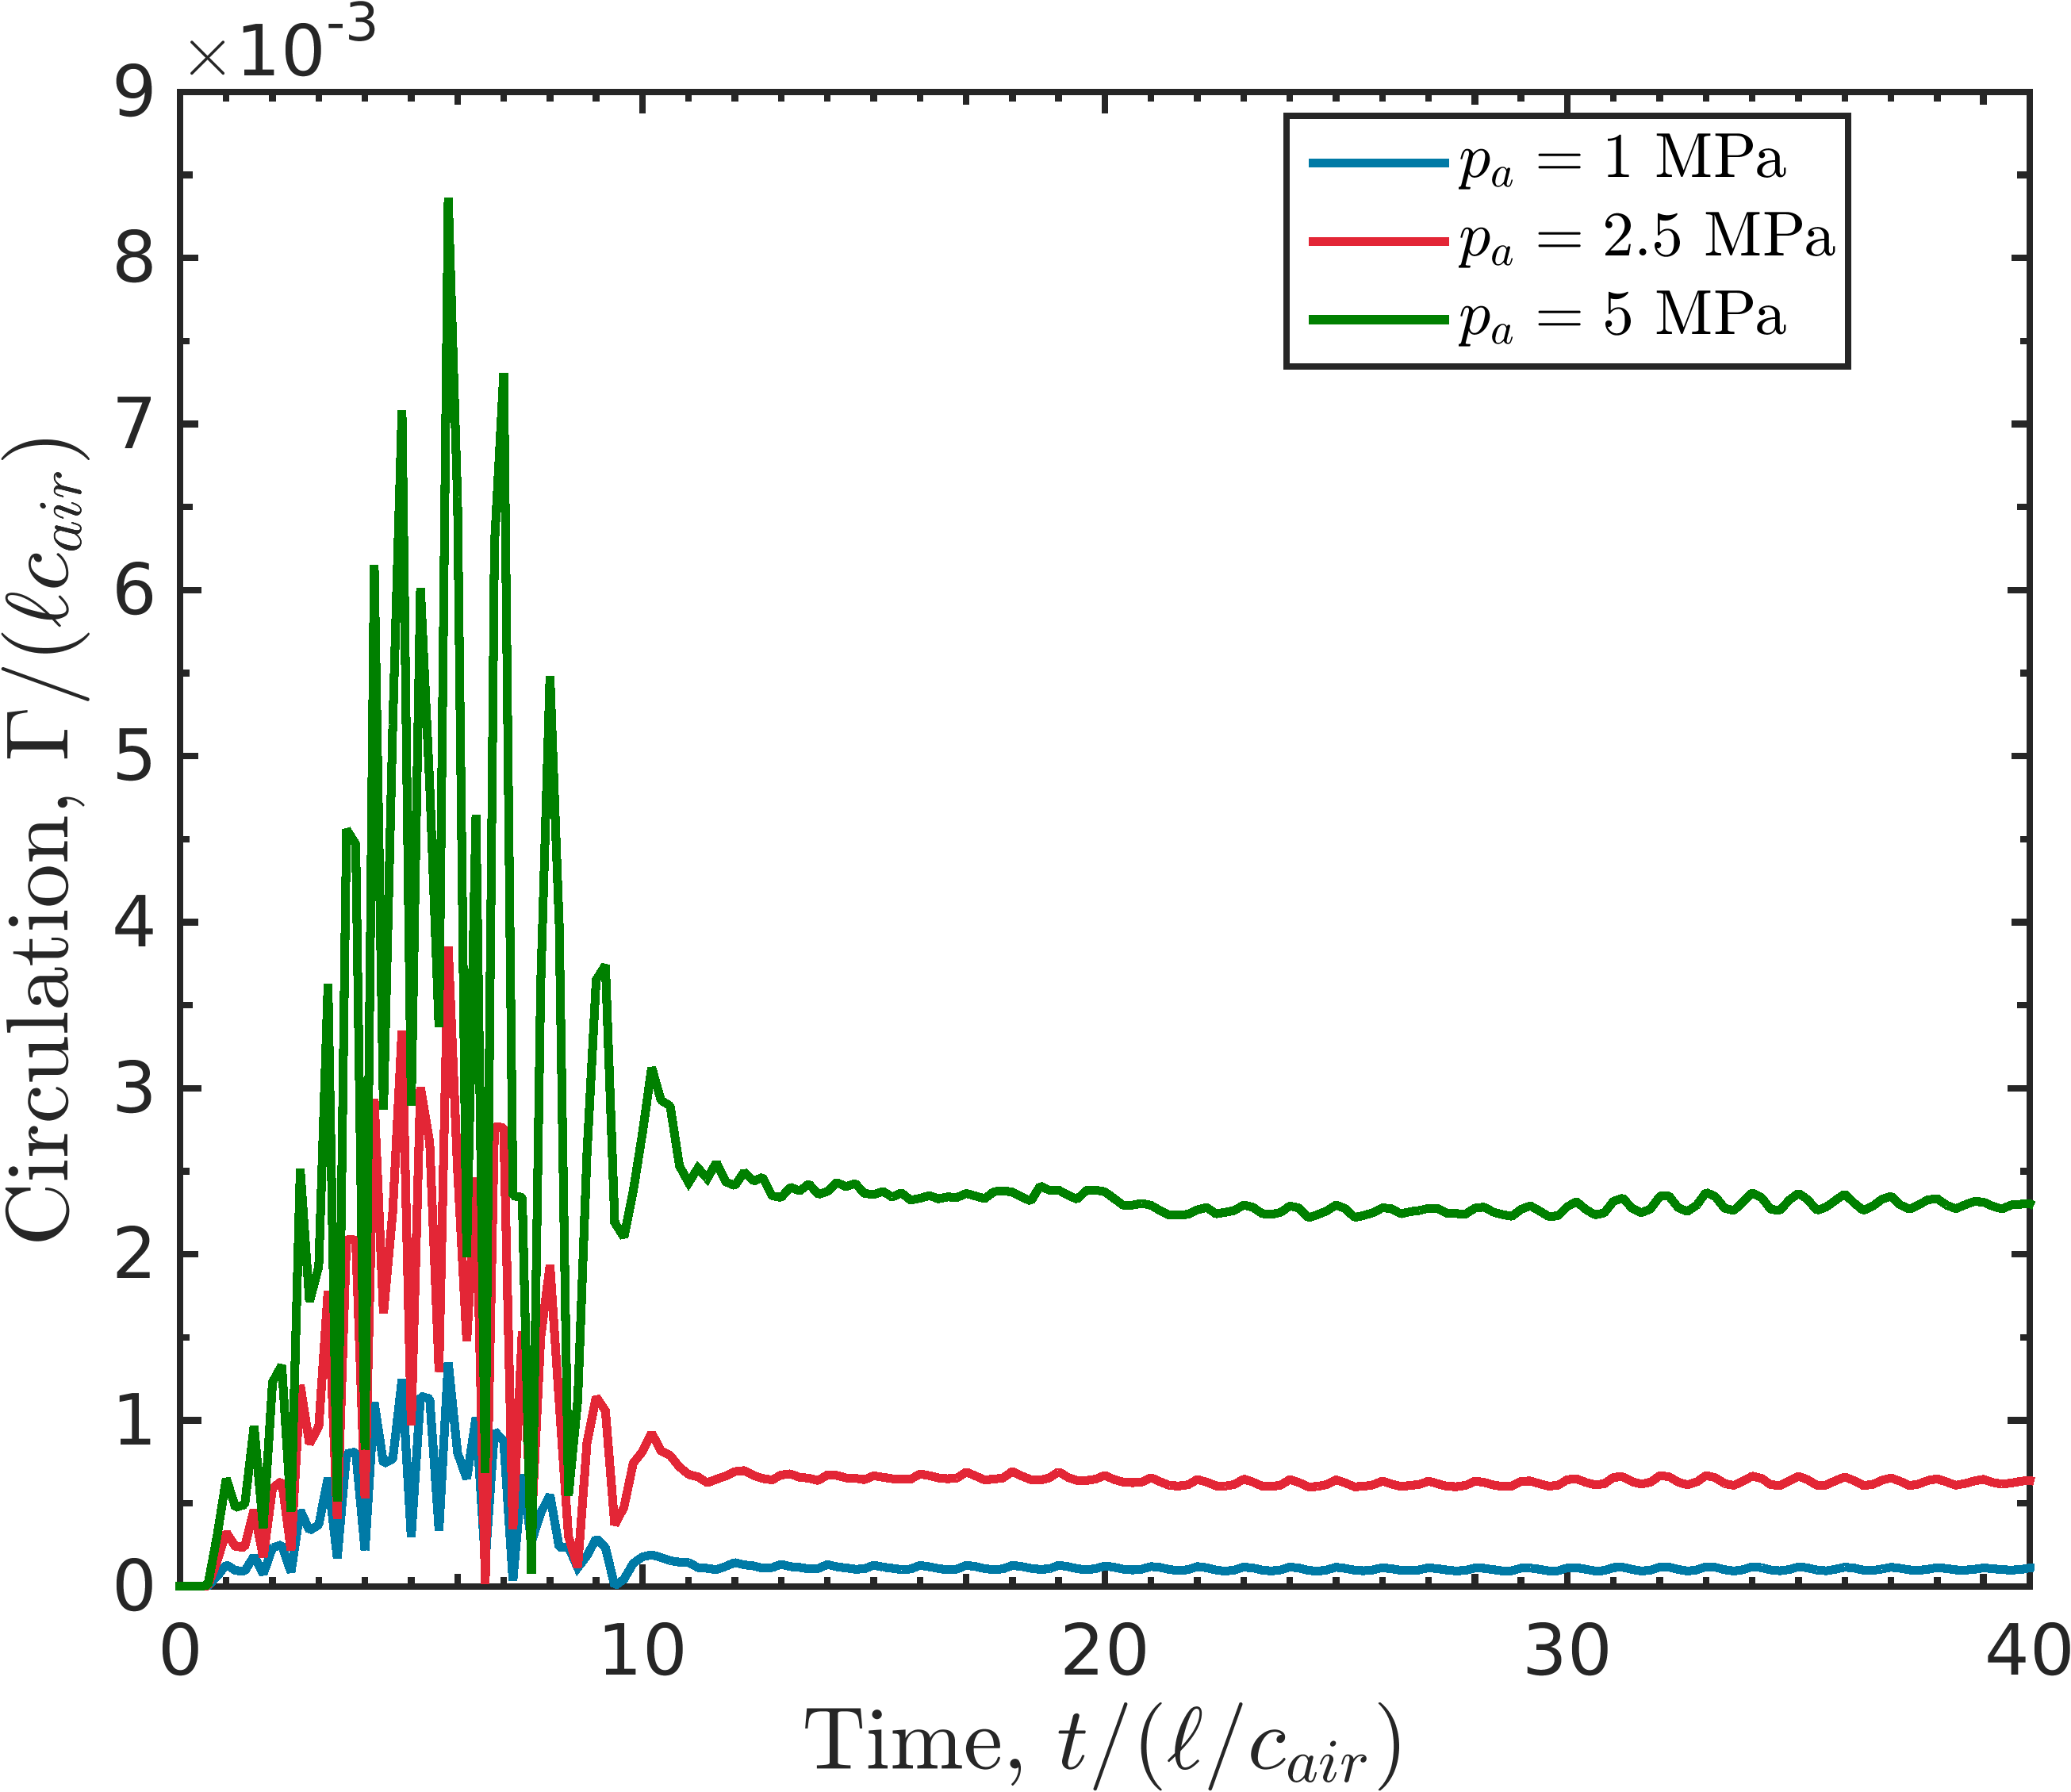
\includegraphics[width=\textwidth]{./figs/lung_figs/rmawave_1_A10,25,50_a30_circulation_01-Mar-2017}
      };%
      \begin{scope}[x={(image.south east)},y={(image.north west)}]%
        \node[font=\normalsize,right] at (0.07,0.13) {};%
      \end{scope}%  
    \end{tikzpicture}%
    \caption{\label{fig:us_circulation_pa_dependence} $p_a = 1, 2.5, 5$ MPa, $a_0 = 0.3\ell$}
  \end{subfigure}
  \caption{Ultrasound-deposited circulation}
  \label{fig:us_circulation_history}
\end{figure}
%
\subsection{Interface strain, $\varepsilon$}
In consideration of strain-induced damage of the alveolar wall, the
linear strain histories $\varepsilon(t)$, as defined in Equation
\eqref{eq:linear_strain}, are plotted for each wave and perturbation
amplitude combination. I will first examine the dependence of strain
on $p_a$ and $a_0$ and then discuss the results in the context of
\ac{DUS}.

To illustrate the dependence of the interface strain on the pulse
amplitude $p_a$, Figure \ref{fig:pa_dependence_strain} plots
$\varepsilon(t)$ for $p_a = 1$ (blue), $2$ (red), and $5$ (green)
MPa. Subfigures \subref{fig:strain_multi-pa_a03},
\subref{fig:strain_multi-pa_a10}, and \subref{fig:strain_multi-pa_a30}
correspond to initial perturbation amplitudes
$a_0 = 0.03\ell, 0.1\ell,$ and $0.3\ell$ respectively. Similarly, to
illustrate the dependence of $\varepsilon$ on the initial perturbation
amplitude $a_0$, Figure \ref{fig:a0_dependence_strain} shows a subset
of this data re-plotted for fixed $p_a$. Strain histories
$\varepsilon(t)$ are shown for $a_0 = 0.03\ell$ (blue), $0.1\ell$
(red), and $0.3\ell$ (green). Subfigures
\subref{fig:strain_multi-a0-A25} and \subref{fig:strain_multi-a0-A50}
correspond to constant $p_a = 2.5$ and $5$ MPa respectively. For all
pressure amplitudes $a_0$ and initial perturbation amplitudes $a_0$,
negative strain is observed during and immediately following the wave
interaction, indicating a net compression of the interface. This
compression is observed to correspond to the flattening of the
interface perturbation during and after the interaction with the
acoustic pulse. For the $p_a = 1$ MPa wave and all $a_0$ and the $2.5$
MPa wave with $a_0 = 0.03\ell$ and $0.1\ell$, this compression is
observed to slowly continue at a decreasing rate throughout the
duration of the simulation. For the $p_a = 2.5$ MPa wave with
$a_0 = 0.1\ell$ and the $p_a = 5$ MPa wave and all $a_0$, the
compression is followed by a net expansion or stretching of the
interface at late times. Based on Figures \ref{fig:rho_snapshots_A25}
and \ref{fig:rho_snapshots_A50} we can see this that this corresponds
to the growth of the aforementioned fluid spike. As we observe that
this deformation and strain increase occur long after the passage of
the wave, when the acoustic pressure is $0$, and as such cannot be
explained by linear acoustics.

Unsurprisingly, the strains observed rise with increasing $p_a$ and
$a_0$. The minimal strain case is observed to occur for
$a_0 = 0.03\ell$ and $p_a = 1$ MPa. For this case, the maximum strain
is observed at the final computed time $t = 500$ is
$\varepsilon-0.001$. The maximum strain case occurs for
$a_0 = 0.3\ell$ and $p_a = 5$ MPa. In the interest of increasing the
relevance of the presented work to \ac{DUS}-induced lung hemorrhage we
consider the presented strain results relative to the $8\%$ strain
failure criteria \citep{Vlahakis2000}. For this case, the maximum
strain observed at the final computed time $t = 500$ and is
$\varepsilon+0.38$. For the cases with $a_0 \geq 0.1\ell$ and
$p_a = 5$ MPa the strain exceeds the $\varepsilon=0.08$ threshold at
$t = 171$ and $t = 377$. For a $200 \mu$m alveolus, this would occur
at approximately $100$ and $220 \mu$s.
%
\begin{figure}
  \centering
  \begin{subfigure}[b]{0.49\textwidth}
    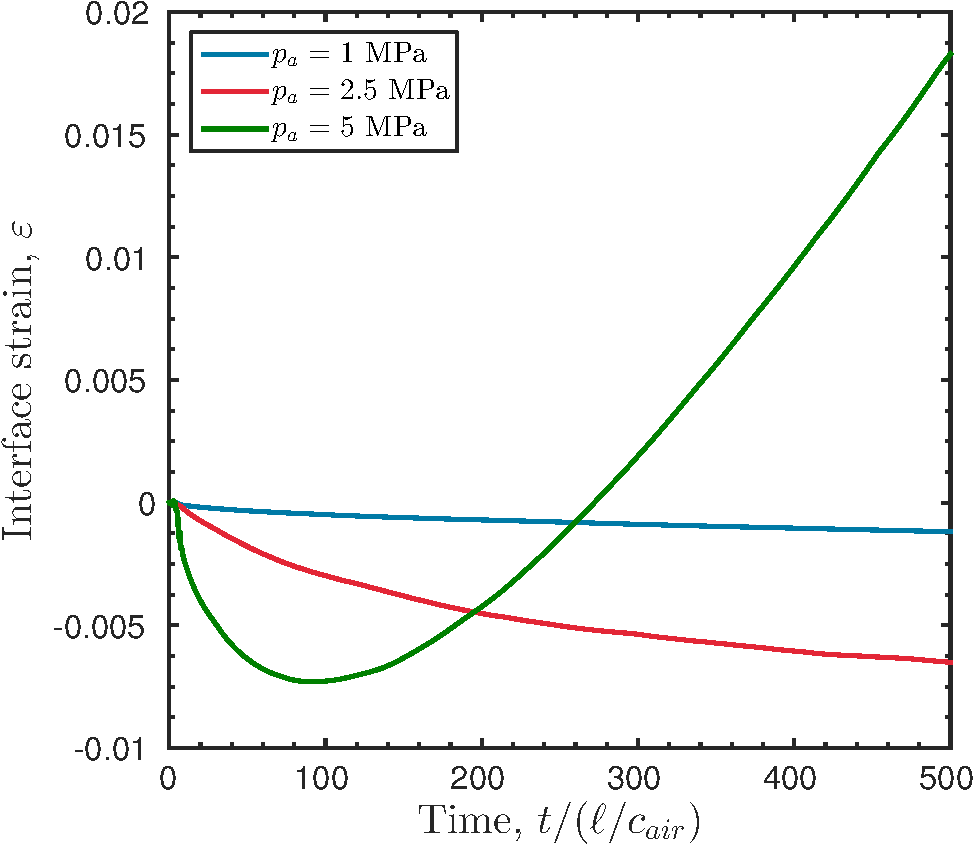
\includegraphics[width=\textwidth]{./figs/lung_figs/rmawave_1_A10,25,50_a03_strain_08-Mar-2017}
    \caption{\label{fig:strain_multi-pa_a03} $a_0 = 0.03\ell$}
  \end{subfigure}
  ~ 
  \begin{subfigure}[b]{0.49\textwidth}
    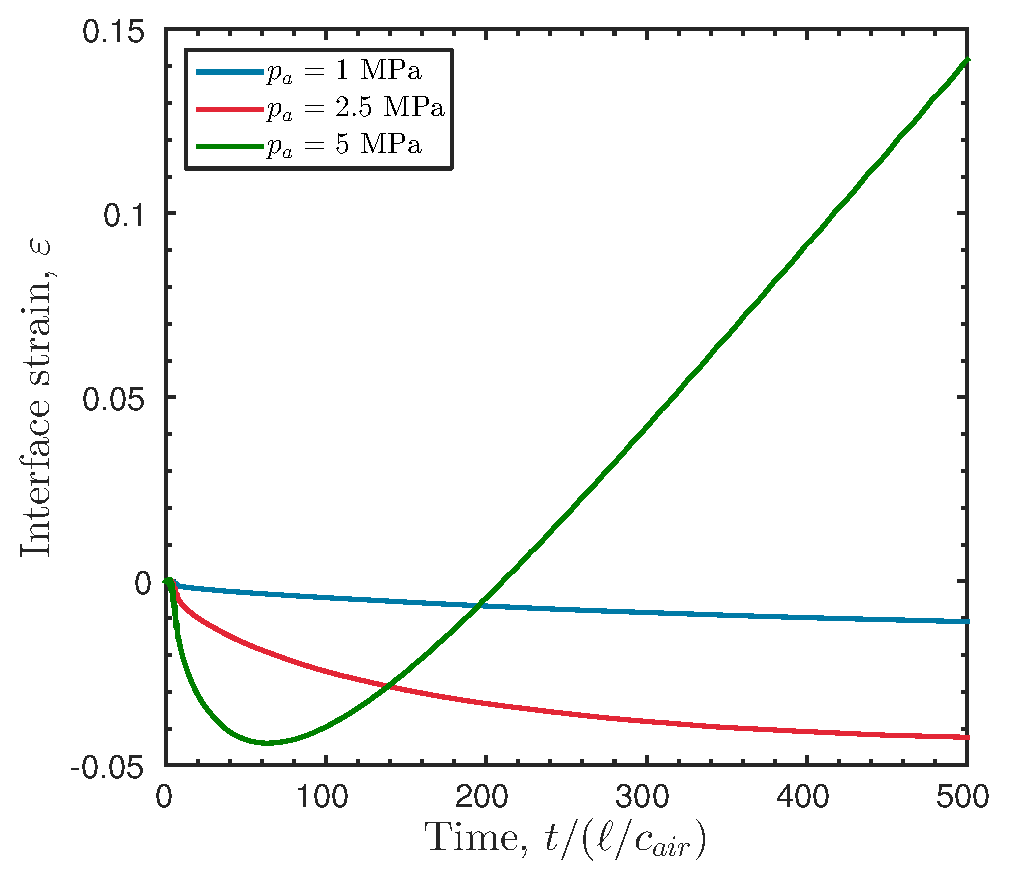
\includegraphics[width=\textwidth]{./figs/lung_figs/rmawave_1_A10,25,50_a10_strain_08-Mar-2017}
    \caption{\label{fig:strain_multi-pa_a10} $a_0 = 0.1\ell$}
  \end{subfigure}
  ~ 
  \begin{subfigure}[b]{0.49\textwidth}
    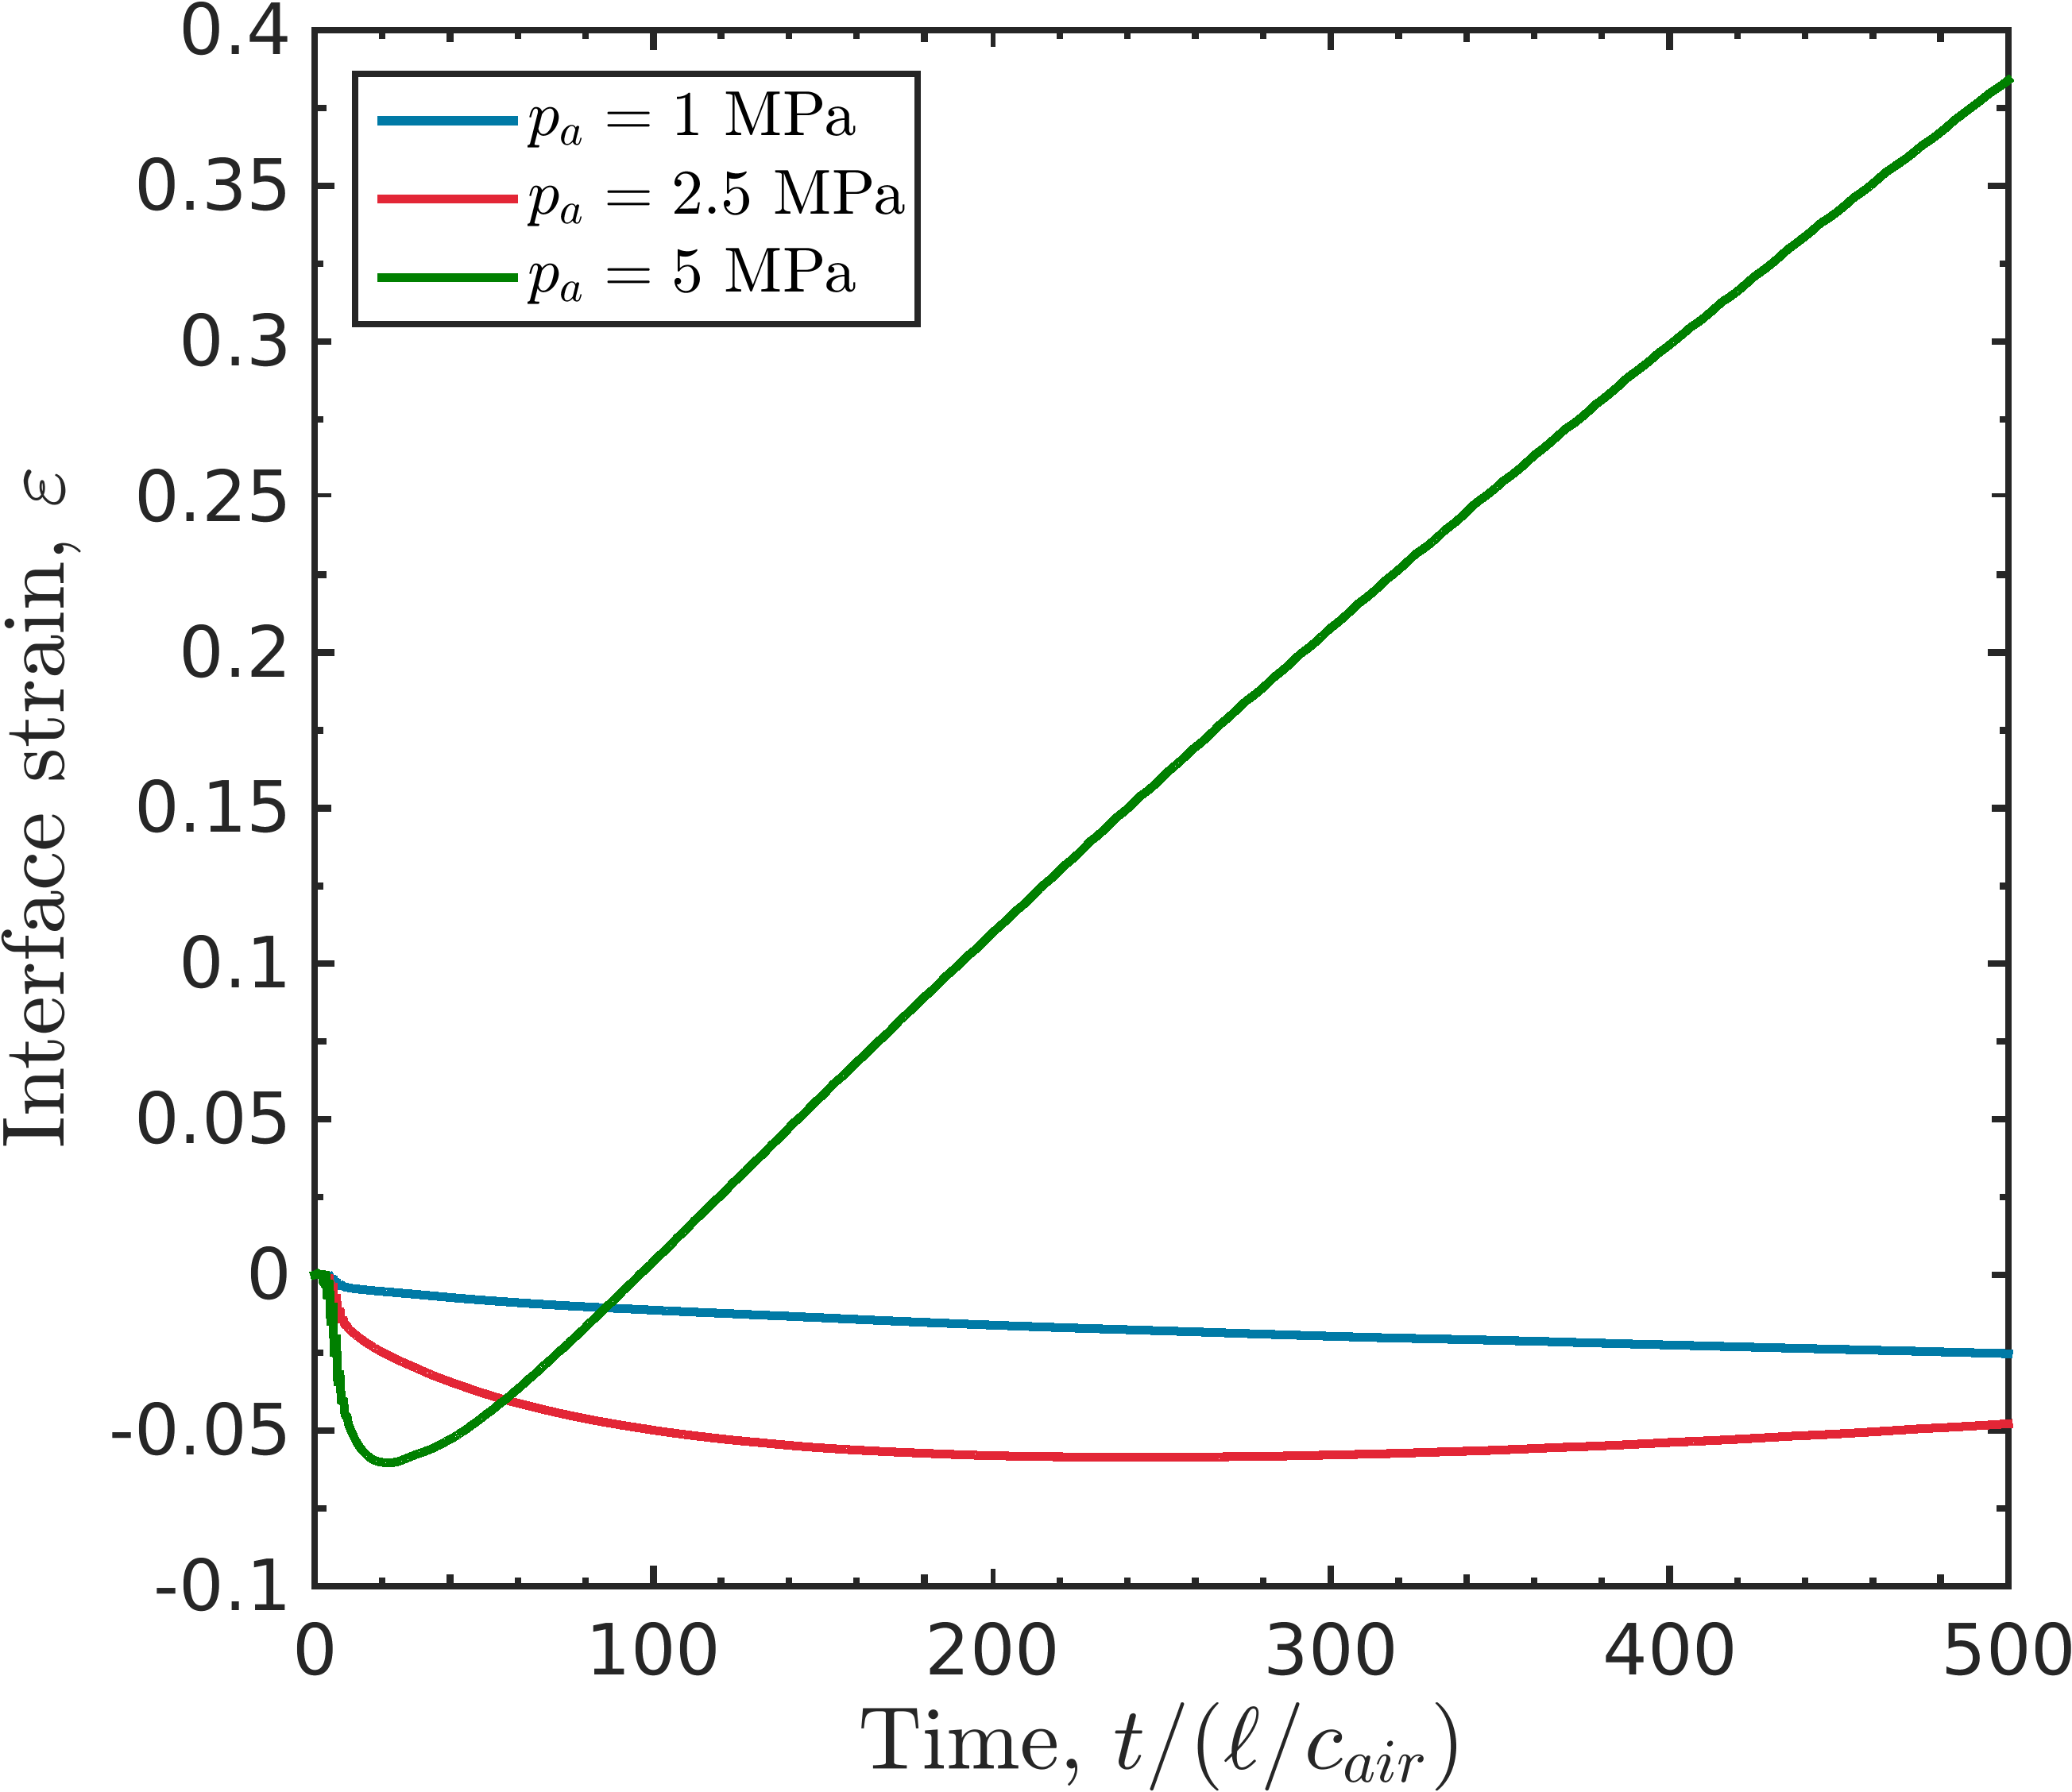
\includegraphics[width=\textwidth]{./figs/lung_figs/rmawave_1_A10,25,50_a30_strain_08-Mar-2017}
    \caption{\label{fig:strain_multi-pa_a30} $a_0 = 0.3\ell$}
  \end{subfigure}
  %
  \caption{To illustrate the dependence of the interface strain on the
    pulse amplitude, the linear strain is plotted as a function of
    time for $t\leq500$ for $p_a=1, 2.5,$ and $5$ MPa pulses. Each plot
    shows $\varepsilon$ for a different initial
    condition. In Figures \subref{fig:strain_multi-pa_a03},
    \subref{fig:strain_multi-pa_a10}, and
    \subref{fig:strain_multi-pa_a30} $a_0=0.03\ell,\, 0.1\ell,$ and
    $0.3\ell$ respectively.}
 \label{fig:pa_dependence_strain}
\end{figure}
%
\begin{figure}
  \centering
  \begin{subfigure}[b]{0.49\textwidth}
    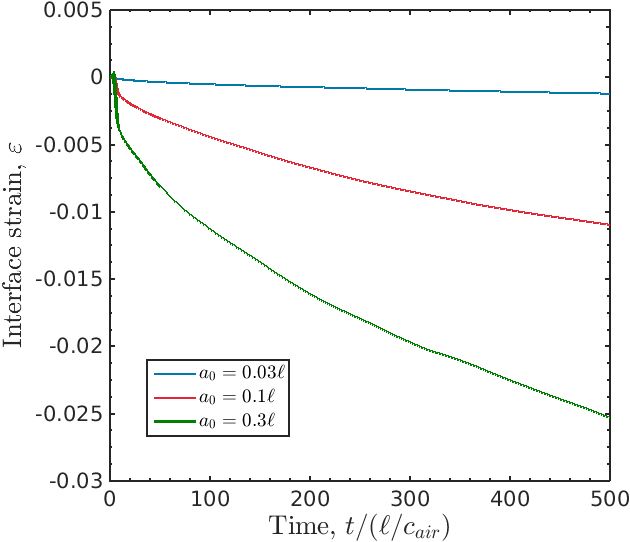
\includegraphics[width=\textwidth]{./figs/lung_figs/rmawave_1_A10_a03,10,30_strain_08-Mar-2017}
    \caption{\label{fig:strain_multi-a0-A10} $p_a = 1.0$ MPa}
  \end{subfigure}
  ~ 
  \begin{subfigure}[b]{0.49\textwidth}
    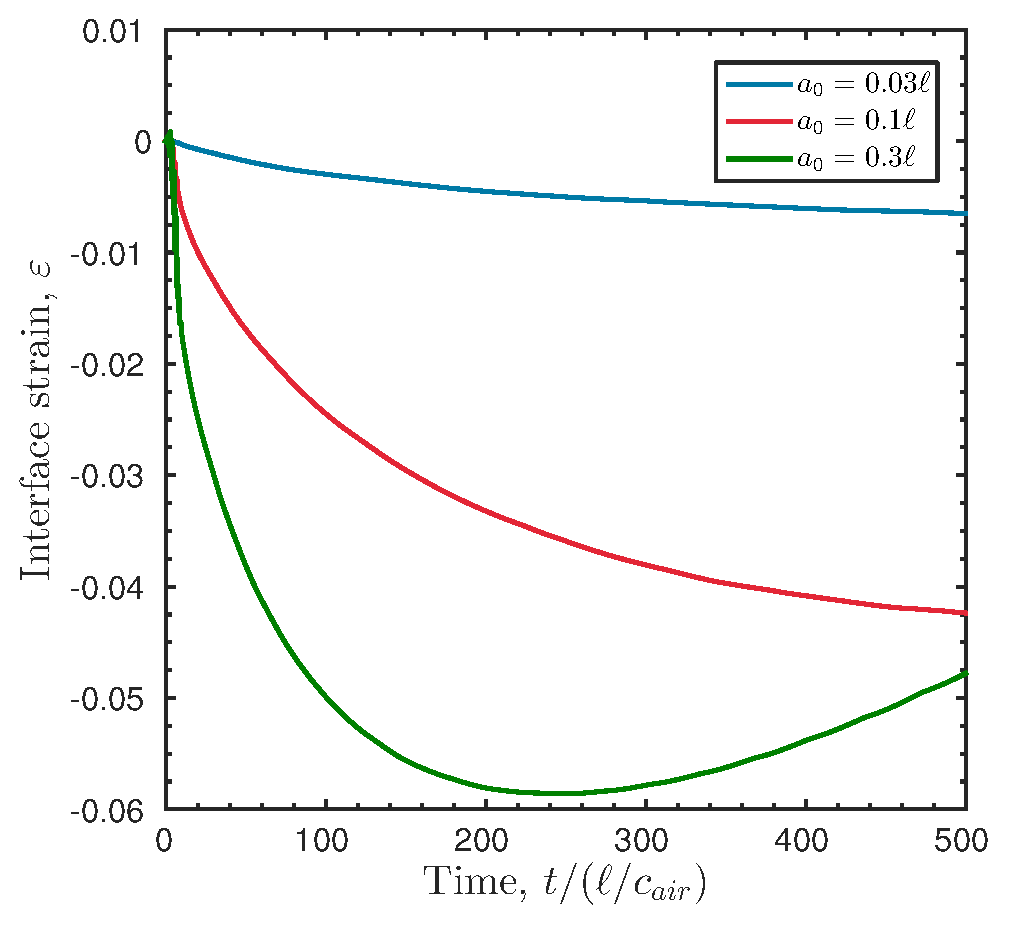
\includegraphics[width=\textwidth]{./figs/lung_figs/rmawave_1_A25_a03,10,30_strain_08-Mar-2017}
    \caption{\label{fig:strain_multi-a0-A25} $p_a = 2.5$ MPa}
  \end{subfigure}
  ~
  \begin{subfigure}[b]{0.49\textwidth}
    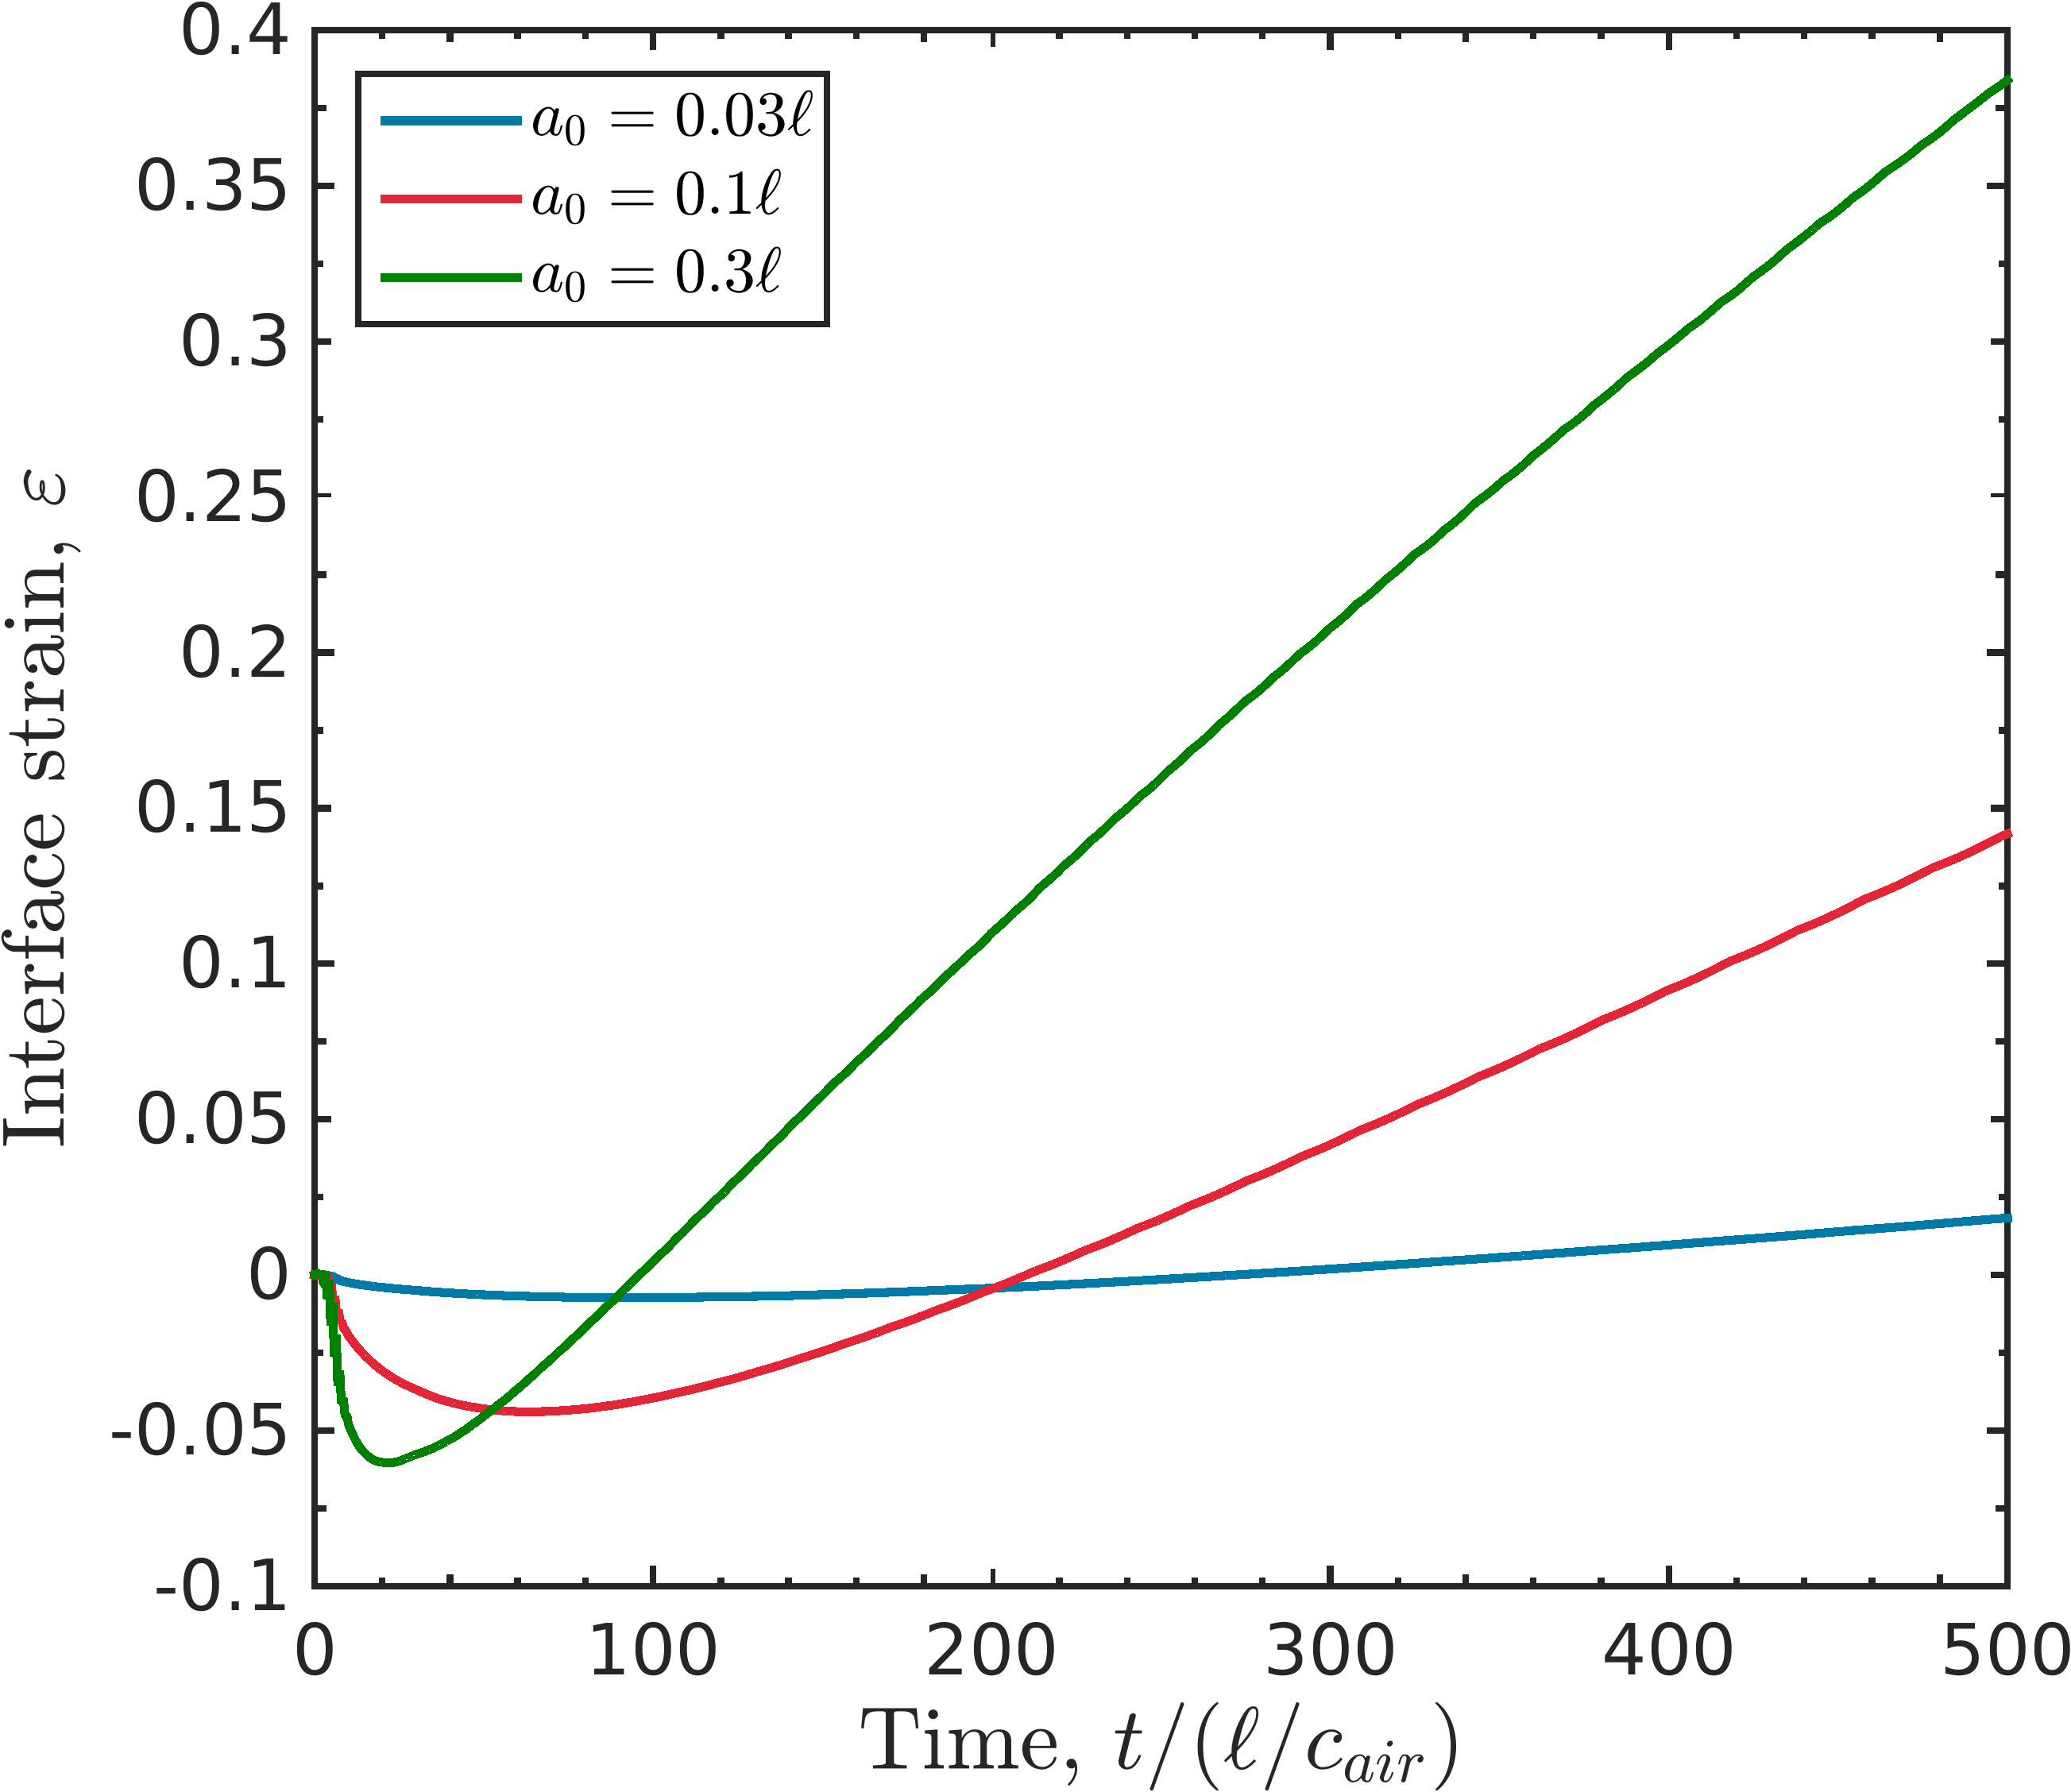
\includegraphics[width=\textwidth]{./figs/lung_figs/rmawave_1_A50_a03,10,30_strain_08-Mar-2017}
    \caption{\label{fig:strain_multi-a0-A50} $p_a = 5$ MPa}
  \end{subfigure}
  % 
  \caption{To illustrate the dependence of the interface strain on the
    initial interface amplitude $a_0$, the linear strain of the
    interface is plotted as a function of time for $t\leq500$ for
    $a_0=0.03\ell, 0.1\ell,$ and $0.3\ell$. Each plot shows $\varepsilon$
    for a different pulse amplitude $p_a$. Figure
    \subref{fig:stress_multi-a0-A25}, $p_a = 2.5$ MPa and in Figure
    \subref{fig:stress_multi-a0-A50}, $p_a = 5$ MPa .}
  \label{fig:a0_dependence_strain}
\end{figure}
%
%
\subsection{Viscous stress}
In consideration of the viscous stress we are primarily interested in
the potential for viscous stress-related damage of the alveolar
walls. Thus we consider the point along the interface, at which the
viscous stress is greatest. We observe, somewhat unsurprisingly, that
this stress occurs during the wave-interface interaction, and in
particular occurs near the point when the maximum pressure amplitude
encounters the interface. To illustrate the viscous stress around the
interface color contours of the viscous stress fields are provided for
the $p_a = 5$ MPa case in Figure \ref{fig:tauxy_snapshots} at $t=5$,
approximately when the acoustic pulse and viscous stress are at their
maximum amplitudes. Subfigures \ref{fig:tauxy_snapshot_A50_a03},
\ref{fig:tauxy_snapshot_A50_a10}, and \ref{fig:tauxy_snapshot_A50_a30}
again correspond to respective initial perturbation amplitudes of
$a_0 = 0.03\ell, 0.1\ell,$ and $0.3\ell$. Black lines indicate
isocontours of the volume fraction of water $y_0 = 0.5$. The maximum
viscous stress is observed to occur in the lighter region of the
interface, in which the fluid is mostly made up of air and the
velocity gradients are higher. At this point in time, the fluid around
the interface has had little time to accelerate as a result of the
wave and consequently the interface remains largely undeformed.

For each of the initial perturbation amplitudes $a_0$, Figure
\ref{fig:pa_dependence_stress} shows the maximum viscous stress
amplitude $\abs{\tau_{xy}}_{max}$ in the field as a function of time
for $p_a = 1$ (blue), $2.5$ (red),and $5$ (green) MPa pulses. During
the wave interaction, $\abs{\tau_{xy}}_{max}$ oscillates with the wave
around a mean value which appears to rise and fall with the acoustic
intensity. For a given $a_0$, barring chronologically local
oscillations, $\abs{\tau_{xy}}_{max}$ increases with increasing $p_a$,
i.e, stronger waves. As $a_0$ is varied for fixed $p_a$, two effects
are observed. First, as $a_0$ increases, the maximum viscous stress
appears less oscillatory, or more precisely, the amplitude of
oscillations in $\abs{\tau_{xy}}_{max}$ relative to the chonologically
local mean, decreases. As a result of the varying degree of
oscillation, the second observation is slightly less obvious from the
figures, which is that as $a_0$ increases, the chronologically local
mean value of $\abs{\tau_{xy}}_{max}$ appears to increase with
increasing $a_0$ as well. After the passage of the wave, the maximum
shear stress drops to nearly zero in all cases.

In consideration of \ac{DUS}, we note that for the parameters
considered here the maximum viscous stress amplitudes observed at the
interface occurred during the interaction with the wave and ranged
from $2 < \left|\tau_{xy}\right| \leq 58$ Pa. This is two orders of
magnitude below the $8$ kPa minimal stress failure threshold observed
by \cite{West1991} for disruption of alveolar epithelium. These
stresses occurred during the wave-interface interaction, and quickly
fell off thereafter, in much less time than a typical period between
pulses ($\sim 1$ ms). This suggests that viscous stresses are not
likely to quickly accumulate between pulses. A possible, exception to
this could occur if the velocity field were to change significantly as
a result of accumulated vorticity from subsequent \ac{US} pulses and
assessment of the feasibility of this is beyond the scope of this
work.
%
%
\begin{figure}
  \centering
  \begin{subfigure}[b]{0.32\textwidth}
    \begin{tikzpicture}%
      \node[anchor=south west,inner sep=0] (image) at (0,0) {
        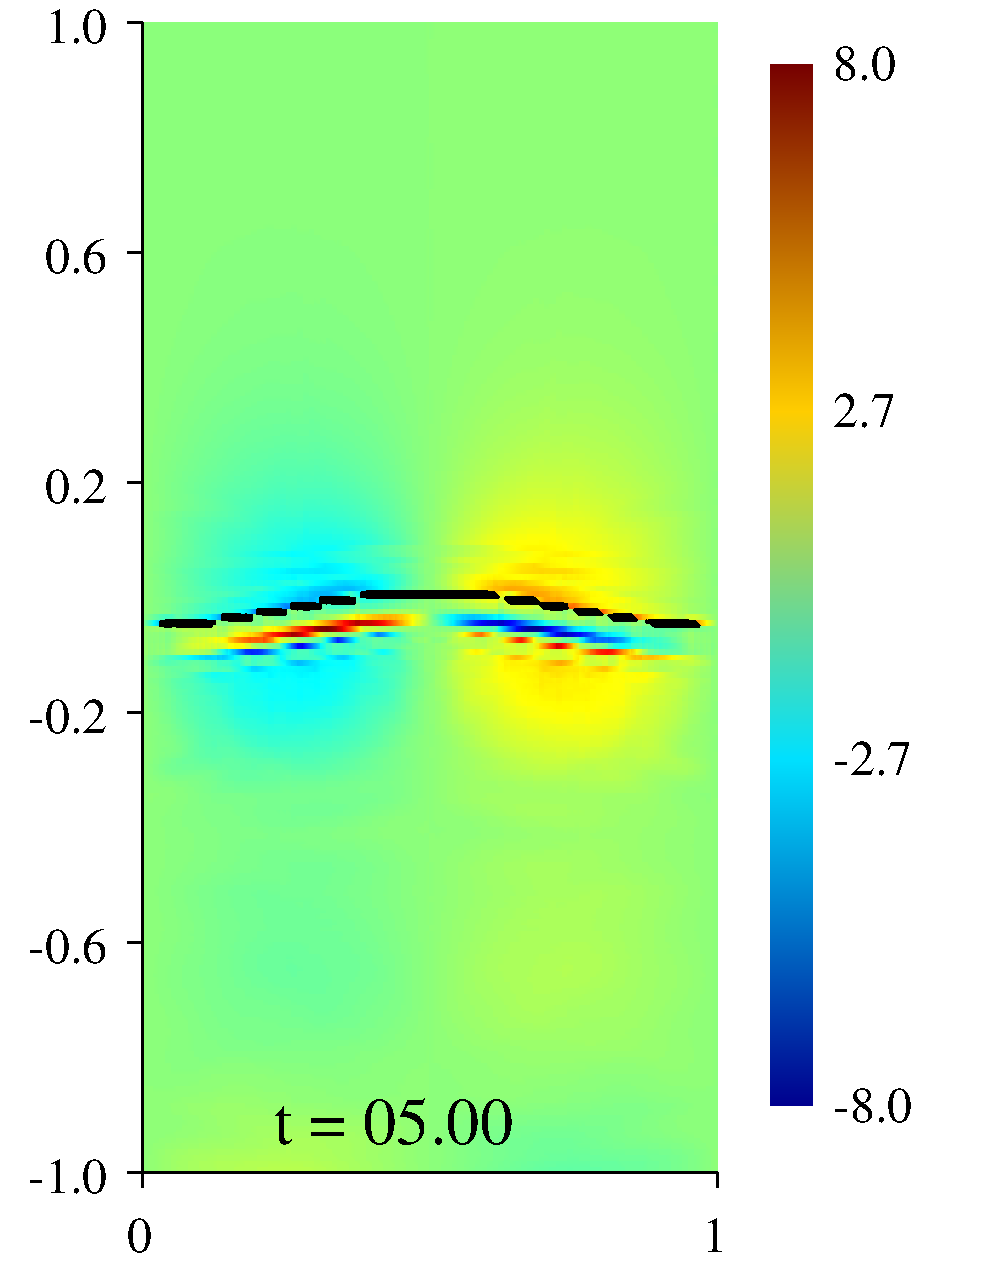
\includegraphics[width=\textwidth]{./figs/lung_figs/rmawave_1_A50_a03_t005_tauxy_snapshots}
      };%
      \begin{scope}[x={(image.south east)},y={(image.north west)}]%
        \node[font=\small,right] at (0.75,0.05) {$\tau_{xy}$ (Pa)};%
      \end{scope}%  
    \end{tikzpicture}%
    \caption{\label{fig:tauxy_snapshot_A50_a03} $a_0 = 0.03\ell$}
  \end{subfigure}
  ~ 
  \begin{subfigure}[b]{0.32\textwidth}
    \begin{tikzpicture}%
      \node[anchor=south west,inner sep=0] (image) at (0,0) {
        \includegraphics[width=\textwidth]{./figs/lung_figs/rmawave_1_A50_a10_t005_tauxy_snapshots}
      };%
      \begin{scope}[x={(image.south east)},y={(image.north west)}]%
        \node[font=\small,right] at (0.75,0.05) {$\tau_{xy}$ (Pa)};%
      \end{scope}%  
    \end{tikzpicture}%
    \caption{\label{fig:tauxy_snapshot_A50_a10} $a_0 = 0.1\ell$}
  \end{subfigure}
  ~ 
  \begin{subfigure}[b]{0.32\textwidth}
    \begin{tikzpicture}%
      \node[anchor=south west,inner sep=0] (image) at (0,0) {
        \includegraphics[width=\textwidth]{./figs/lung_figs/rmawave_1_A50_a30_t500_tauxy_snapshots}
      };%
      \begin{scope}[x={(image.south east)},y={(image.north west)}]%
        \node[font=\small,right] at (0.75,0.05) {$\tau_{xy}$ (Pa)};%
      \end{scope}%  
    \end{tikzpicture}%
    \caption{\label{fig:tauxy_snapshot_A50_a30} $a_0 = 0.3\ell$}
  \end{subfigure}
  % 
  \caption{Contour plots of the Newtonian viscous stress $\tau_{xy}$
    in Pascals are shown for each initial perturbation amplitude for
    the $p_a=5$ MPa pulse at $t=5$, near the point when the maximum
    stress occurs. In Figures \subref{fig:tauxy_snapshot_A50_a03},
    \subref{fig:tauxy_snapshot_A50_a10}, and
    \subref{fig:tauxy_snapshot_A50_a30} $a_0=0.03\ell,\, 0.1\ell,$ and
    $0.3\ell$ respectively.  }
  \label{fig:tauxy_snapshots}
\end{figure}
% 
\begin{figure}
  \centering
  \begin{subfigure}[b]{0.49\textwidth}
    %\includegraphics[width=\textwidth]{./figs/lung_figs/rmawave_1_A10,25,50_a3_tauxy_27-Feb-2017}
    \includegraphics[width=\textwidth]{./figs/lung_figs/rmawave_1_A10,25,50_a03_tauxy_07-Mar-2017}
    \caption{\label{fig:stress_multi-pa_a03} $a_0 = 0.03\ell$}
  \end{subfigure}
  ~ 
  \begin{subfigure}[b]{0.49\textwidth}
    \includegraphics[width=\textwidth]{./figs/lung_figs/rmawave_1_A10,25,50_a10_tauxy_27-Feb-2017}
    \caption{\label{fig:stress_multi-pa_a10} $a_0 = 0.1\ell$}
  \end{subfigure}
  ~ 
  \begin{subfigure}[b]{0.49\textwidth}
    \includegraphics[width=\textwidth]{./figs/lung_figs/rmawave_1_A10,25,50_a30_tauxy_27-Feb-2017}
    \caption{\label{fig:stress_multi-pa_a30} $a_0 = 0.3\ell$}
  \end{subfigure}
  % 
  \caption{To illustrate the dependence of the viscous stress on the
    pulse amplitude, the Maximum shear stress in the field is is
    plotted as a function of time for $t\leq40$ for $p_a=1, 2.5,$ and
    $5$ MPa pulses. Each plot shows $\left|\tau_{xy}\right|_{max}$ for
    a different initial condition. In Figures
    \subref{fig:stress_multi-pa_a03},
    \subref{fig:stress_multi-pa_a10}, and
    \subref{fig:stress_multi-pa_a30} $a_0=0.03\ell,\, 0.1\ell,$ and
    $0.3\ell$ respectively.}
  \label{fig:pa_dependence_stress}
\end{figure}
%
\begin{figure}
  \centering
  \begin{subfigure}[b]{0.49\textwidth}
    \includegraphics[width=\textwidth]{./figs/lung_figs/rmawave_1_A25_a3,10,30_tauxy_27-Feb-2017}
    \caption{\label{fig:stress_multi-a0-A25} $p_a = 2.5$ MPa}
  \end{subfigure}
  ~ 
  \begin{subfigure}[b]{0.49\textwidth}
    \includegraphics[width=\textwidth]{./figs/lung_figs/rmawave_1_A50_a3,10,30_tauxy_27-Feb-2017}
    \caption{\label{fig:stress_multi-a0-A50} $p_a = 5$ MPa}
  \end{subfigure}
  % 
  \caption{To illustrate the dependence of the viscous stress on the
    initial interface amplitude $a_0$, the Maximum shear stress in the
    field is plotted as a function of time for $t\leq40$ for
    $a_0=0.03\ell, 0.1\ell,$ and $0.3\ell$. Each plot shows
    $\left|\tau_{xy}\right|_{max}$ for a different pulse amplitude $p_a$. In
    Figure \subref{fig:stress_multi-a0-A25}, $p_a = 2.5$ MPa and in
    Figure \subref{fig:stress_multi-a0-A50}, $p_a = 5$ MPa .}
  \label{fig:a0_dependence_stress}
\end{figure}
%
%
%
%

\subsection{Results summary and further Discussion}
\label{sec:usbe_lung_bio}
In summary, \ac{US} pulse waves were simulated propagating from water
into sinusoidal air-water interfaces to model a single \ac{US}-pulse
impinging upon an alveolus from surrounding soft tissue. Nine cases
were considered in which pulses of peak pulse amplitudes of
$p_a = 1, 2.5,$ and $5$ MPa pulses were each propagated at interfaces
of perturbation amplitude $a_0= 0.03\ell, 0.1\ell,$ and $0.3\ell$. For
a typical alveolar size of $200 \mu$m, the maximum simulation time was
approximately $300 \mu$s. Relevant calculations of the density fields,
viscous stress fields, vorticity fields, and interface strain within
the simulated period are reported. For each case, vorticity was
observed to be generated at the interface by the wave-interface
interaction with varying amounts of total circulation remaining after
the passage of the wave. The interfaces continued to deform after the
passage of the wave. The computed peak interface strain amplitudes
ranged from $0.01 \leq \varepsilon \leq 0.38$. Only for the $5$ MPa
did a single pulse induce strains exceeding the 8\% threshold
\citep{Vlahakis2000} during the computed period. The computed peak
stresses were of order $\sim\orderof{Pa}$, far below the $8$ kPa
stress failure criterion \citep{West1991}.

This work is a first step toward investigating the possibility of
baroclinic vorticity in the lungs as potential mechanism of
ultrasound-induced alveolar hemorrhage. However, the approximation of
the alveolar wall as a Newtonian fluid with properties estimated
between air and water does not capture the true complexity of the
system.  As such, there are unsurprisingly several limitations to this
study that do not allow the simulated physics to fully capture the
physics of diagnostic ultrasound-alveolar interactions. These
limitations, include but are not limited to: a simplification of the
geometry that does not capture the inhomogeneity or 3D nature of the
physical problem; physical effects including such as surface tension,
elasticity, viscosity, and heat transfer are neglected; the use of a
single ultrasound pulse is used instead of many consecutive pulses, as
occurs in diagnostic ultrasound.

Based on our physical understanding understanding, it is not
unreasonable to speculate about how each of these limitations is
likely to effect the simulated physics. While the geometry used in
this study is overly simple, it also reflects what could be as a
\textit{best case scenario} in terms of baroclinic vorticity
generation. The orientation of the mean interface and small
perturbation amplitudes relative to what is actually seen in alveoli
create a somewhat minimal misalignment between the interface density
gradient and \ac{US} pressure gradient, resulting in potentially less
baroclinic vorticity generation for a given wave than might be
expected. The physical effects neglected largely work in favor of
increasing the simulated baroclinic vorticity and subsequently driven
interface growth. We expect that viscous effects will dissipate the
kinetic energy of the observed vorticies as heat. However the
timescales over which this dissipation occurs are \hl{FIGURE THIS
  OUT}. The elasticity of the alveolar wall is expected to induce an
elastic stress in the wall, compression, followed by tension based on
the observed strain curves, which will resist the motion of the
wall. While this tensile stress may be an additional mechanism of
damage, the strain in the alveolar wall is likely to be less than
calculated here. \hl{SURFACE TENSION} Additionally, this model does not allow for the
possibility of mechanical failure of the interface and resulting
discontinuities and hemorrhage into the alveolar space. 

Based on our observed results the use of many sequential pulses in
physical diagnostic ultrasound is one that may have significant impact
on the vorticity and interface dynamics. As we have observed in our
work, vorticity left after the passage of the ultrasound led to
significant deformation of the interface, over time periods far less
than the time periods that occur between subsequent \ac{US}
pulses. The potential for accumulation of vorticity, and increased
deformation seems plausible based on our results. The ability to
capture failure behavior is likely to be particularly important in the
case multiple pulses with more realistic geometries, because failure
of the interface and subseqent hemorrhage into the alveolar airspace
may allow for a means by which ultrasound-induced hemorrhage can
propagate into additional alveolar layers.

In addition to the limitations of the present work, there are
definitive limitations of the existing body of knowledge on the
mechanical properties and failure behavior of alveolar tissue under
stresses and strains within the ultrasonic regimes. Poor
characterization of the viscoelastic behavior of alveolar walls makes
determining which physical effects govern the behavior of the system
uncertain. Additionally, the available stress and strain failure
criteria for alveoli are based on much slower processes than occur
during \ac{DUS}, making for an imperfect comparison at best.

%%%%%%%%%%%%%%%%%%%%%%%%%%%%%%% 
\section{conclusions and future work}
While the calculated stresses and strains observed based the
interaction between an air water interface and a single ultrasound
pulse may be representative of a portion the of the physics associated
with \ac{DUS}-alveolar interactions, we cannot confidently say that
baroclinic vorticity is the likely cause of \ac{DUS}-induced
hemorrhage in the lung. We can however draw \hl{three} conclusions from this work. 
\begin{enumerate}
\item Newtonian, viscous stress alone is unlikely to be sufficient to cause \ac{DUS}-induced hemorrhage of the alveolar wall.
\item \ac{DUS} pulses within clinically relevant regimes have the potential to deposit baroclinic vorticity within gas-liquid interfaces in the lungs.
\item \hl{Vorticity may be capable of deforming gas-liquid interfaces in the lungs.}
\end{enumerate}












% \begin{comment}
%   % \section{Results and discussion}
%   % \subsection{Stresses and strains in the lungs}
%   % Lung tissue has been recognized to exhibit viscoelastic behavior
%   % since as early as 1939 \citep{Bayliss1939}. As a result of this,
%   % we consider both viscous and elastic stress as potential damage
%   % mechanisms underlying ultrasound-induced lung hemorrhage.

%   % \subsubsection{Viscous Stresses}
%   % \begin{figure}
%   %   \centering
%   %   \includegraphics{./figs/placeholder}
%   %   \caption{Plot of maximum viscous stress vs time for US pulse
%   %   waveforms.}
%   % \end{figure}

%   % \subsubsection{Elastic Stresses}
%   % \begin{figure}
%   %   \centering
%   %   \includegraphics{./figs/placeholder}
%   %   %   \caption{Plot of engineering strain vs time. Strain on left
%   %   %   side, stress on right side, dashed line at 500 kPa, which is
%   %   %   failure based on \cite{West1999}.}
%   % \end{figure}
% \end{comment}


% \begin{comment} %This is pretty much all in the previous chapter
%   The physical mechanisms underlying \ac{DUS}-induced \ac{PH} are not
%   well understood and traditionally expected \ac{US} bioeffects
%   mechanisms do not appear to be the primary cause of damage. \ac{US}
%   bioeffects mechanisms are typically classified as thermal or
%   non-thermal with the bulk of non-thermal bioeffects being a result
%   of acoustic \ac{IC}. \cite{Zachary2006} finds that \ac{DUS}-induced
%   lung lesions do not appear similar to those induced by heat and
%   concludes that thermal mechanisms are not likely to be the
%   cause. \cite{OBrien2000} observes that the severity of
%   \ac{DUS}-induced \ac{LH} in mice increases under raised hydrostatic
%   pressure, and \cite{Raeman1996} finds that the \ac{LH} is unaffected
%   by the introduction of \ac{US} contrast agents. Both of these
%   findings are inconsistent with what would be expected of
%   \ac{IC}-induced hemorrhage. One study reports detecting cavitation
%   during \ac{DUS}-lung interaction in rats
%   \cite{Holland1996}. \cite{Tjan2007} considers another potential
%   damage mechanism, that focused \ac{US} may lead to the ejection of
%   droplets capable of puncturing the air-filled sacs within the
%   lung. To investigate this, they perform numerical simulations of as
%   an inviscid, free surface subjected to a Gaussian velocity potential
%   and show show that the proposed droplet ejection may occur under
%   certain circumstances. Similarly, \cite{Simon2012} observed
%   \ac{HIFU} induced atomization of tissue at air interfaces. Despite
%   these efforts, the precise damage mechanism underlying
%   \ac{DUS}-induced \ac{LH} is still unknown.
% \end{comment}

% % This is probably all in the last chapter or the introduction. Just add a paragraph relating the last chapter to this one here
% \begin{comment}
%   Previously there has been extensive research
%   investigating interactions between fluid-fluid interfaces driven by
%   mechanical waves. Much of this work has been motivated by man-made
%   applications such as inertial confinement fusion and astrophysical
%   phenomena such as supernova collapse. Accordingly much of the previous
%   research has focused on shock-accelerated, perturbed interfaces
%   between fluids of different densities
%   \citep{Brouillette2002}. \cite{Taylor1950} performed linear stability
%   analysis for the case of a perturbed interface between two fluids
%   undergoing constant acceleration, e.g., gravity. Taylor found that
%   under certain configurations the interface perturbation
%   grows. \cite{Richtmyer1960} extended this linear analysis to the case
%   of an impulsively accelerated interface to create a model for the
%   initial growth of a shock-driven interface perturbation. Later,
%   \cite{Meshkov1969} experimentally confirmed Ricthmyer's qualitative
%   predictions. Hence the growth of a shock-driven fluid-fluid interface
%   has been labeled as the \ac{RMI}. To lend physical insight into the
%   underlying mechanism behind this, \cite{Hawley1989} demonstrated that
%   this phenomenon could be described using vortex deposition-evolution
%   paradigm. The basic mechanism driving the growth of the perturbation
%   in the case of the \ac{RMI} is baroclinic vorticity created by the
%   misalignment of the pressure gradient across the shock and the density
%   gradient at the interface. Recently \hl{Patterson \& Johnson
%     (submitted, 2016)} performed numerical experiments and analysis to
%   show that for the case of liquid-gas interfaces, acoustic waves may
%   also be capable of depositing sufficient baroclinic vorticity at the
%   interface to cause significant deformation, as a result of the sharp
%   density gradient across the interface.
% \end{comment}


% \begin{comment}
%   % \subsection{Summary}
%   As \ac{DUS} of the lung has been shown to trigger same-day, acute
%   alveolar hemorrhage \cite{Zachary2001}, it is specifically
%   interactions between the an aveolus and a single \ac{DUS} pulse that
%   we consider in this work. To investigate the mechanism underlying this
%   hemorrhage, we develop a numerical model of this problem to compute
%   the expected dynamics of the alveolar air-tissue interface for varying
%   acoustic amplitudes an alveolar geometries. To relate the computed
%   dynamics to lung hemorrhage, we approximate the relevant stresses and
%   strains and compare these results to existing values of the material
%   properties alveolar tissue to assess possible causes of hemorrhage.

%   \hl{OUT OF PLACE:\\
%     This work aims to use numerical simulations to investigate the
%     dynamics associated with the interaction between an ultrasound pulse and
%     an aleolar air-tissue interface. We hypothesize that acoustically
%     generated baroclinic vorticity within the lungs is capable of driving
%     deformation of alveolar air-tissue interfaces to the point of
%     hemorrhage. We model the problem as a sinusoidally perturbed air-water
%     interface driven by a single acoustic pulse and study the subsequent
%     dynamics. Calculated stresses and strains are compared to previously
%     measured failure criteria from the literature.}

% \end{comment}

% % This is the old methods section, that now largely exists in the previous chapter.
% \begin{comment}
%   \section{Methods}
%   In this section we develop a model of \ac{DUS}-alveolus interaction
%   as a compressible fluid system. We then describe in detail the setup
%   of the numerical experiments performed and calculations performed to
%   investigate the problem. 

%   \subsection{A model of \ac{DUS}-alveolus interaction}
%   \hl{COPIED THIS PARAGRAPH TO OTHER PAPER}.  Consider a \ac{DUS} pulse
%   as it travels into the lungs. After passing through layers of soft
%   tissue and fluid, the wave encounters a network of openly connected,
%   air-filled saccules with distinctly irregular surfaces. These are the
%   alveoli. It is the interaction between an incident \ac{US} pulse and
%   the first alveolar tissue-air interface it encounters that we treat
%   here, as shown in figure \ref{fig:alveolar_schematic}.

%   To model the problem, we consider a rectangular domain with a 2D
%   $(x,y)$ cross section containing soft tissue (modeled as water)
%   sitting atop a single alveolus (modeled as air) as illustrated in
%   figure \ref{fig:ic_schematic}. An acoustic pulse is prescribed within
%   the water, above the interface, and allowed to propagate downward
%   ($-y$-direction) toward the air. The alveolus spans the width of the
%   domain, $\ell$. A typical mean aveolar diameters in an adult human is
%   $200 \mu$m \citep{Ochs2004}.

%   To capture the irregular shape of the alveolus, the water-air
%   interface contains a single mode sinusoidal perturbation of amplitude
%   $a_0$ such that the vertical center of the interface is described by,
%   \begin{align} %Not y_interface in the code
%     Y(x,t=0)_{interface} = a_0\sin\left(\frac{2\pi x}{\ell}-\frac{\pi}{2}\right). 
%   \end{align}
%   An interface thickness $\delta=0.08$ is chosen such that at $t=0$, the
%   fluid in the domain above $y\geq Y_{interface}+\delta/2$ is pure
%   water, and below $y\leq Y_{interface}-\delta/2$ is pure air, which a
%   water-air mixture filling the region around the interface. A more
%   detailed treatment of the interface can be found in referred to
%   \hl{(Patterson and Johnsen, 2016)}. To investigate the dependence of
%   the dynamics on the alveolar geometry we will consider multiple
%   interface perturbation amplitudes: $a_0=0.03\ell, 0.1\ell, 0.2\ell,$
%   and $0.3\ell$.

%   The diagnostic ultrasound pulse is modeled as a sinusoidal carrier
%   wave of amplitude $p_a$ and frequency $f$ modulated by a Gaussian
%   Envelope such that,
%   \begin{align}
%     p(x,t_0) = p_a\sin{\left(2\pi f\frac{\left[y-\left(Y_{wave}+L_{wave}\right)\right]}{c}\right)}\exp{\left(-\frac{\left(\left[y-\left(Y_{wave}+L_{wave}/2\right)\right]c\right)^2}{FWHM/\left(2\sqrt{2\ln{\left(2\right)}} \right)}\right)}.%
%   \end{align}
%   The carrier wavelength $\lambda=c_{water}/f$ and the full width of the
%   Gaussian envelope at half of the maximum amplitude $FWHM$ are designed
%   to scale appropriately with respect to $\ell$. Here,
%   $f\approx 1.25 c_{water} / 2\pi \ell$ and $FWHM=15\ell$. For an
%   alveolar length scale of $\ell=200 \mu$m, this corresponds to $f=1.65$
%   MHz and $FWHM=3$ mm. $L_{wave}=45\ell$ is the length of the
%   computational domain, over which the wave is defined to exist and
%   $Y_{wave}$ is $y$-location of the bottom of the wave at $t=0$, which
%   is set to $10a_0$ above the peak of the interface. To consider the
%   dependence of the interface dynamics on pulse amplitude we vary
%   $p_a = 1, 5, 10,$ and $15$ MPa.

%   \subsection{Governing Equations}
%   To simulate the model problem described above we solve equations for
%   conservation of mass, momentum, energy. While it has been long since
%   recognized that tissue exhibits viscoelastic behavior
%   \citep{Bayliss1939}. To simplify things we consider the expected
%   length scale over which viscosity will influence the dynamics,
%   $l_{viscous}$. From dimensional analysis, this scales as
%   $l_{viscous}\sim\sqrt{\nu/(\ell/c)}$. In air at 300 K,
%   $l_{viscous}\sim\orderof{1 \mu\text{m}}$ and in water
%   $l_{viscous}\sim\orderof{0.1 \mu\text{m}}$. In either case we consider
%   that $l_{viscous}<<\ell$. \hl{Furthermore, we consider the relative
%     importance of elasticity and surface tension }

%   \begin{comment}
%     \begin{itemize}
%     \item $c_{air} = 347.2$ m/s
%     \item $c_{water} = 1500$ m/s
%     \item $\nu_{air} = 1.568\times 10^{-5}$ m$^2$/s
%     \item $\nu_{water} = 0.8539\times 10^{-6}$ m$^2$/s
%     \item $G_{alveolar-wall} = 5$ kPa \cite{Cavalcante2005}
%     \item $\sigma_{water}=0.072$ at N/m 298K
%     \item $\rho_{air}=1.1765$ kg/m$^3$
%     \item $\rho_{water}=996$ kg/m$^3$
%     \item if $p_a=1 MPa$:
%       \begin{itemize}
%       \item $u_{acoustic-water}\approx0.6$ m/s
%       \item $u_{acoustic-air}\approx1.2$ m/s
%       \end{itemize}
%     \item $Re=\frac{\rho u}{\nu}$ =
%     \item $We=\frac{\rho u^2 \ell}{\sigma}$ = $(\infty)_{air}$ =
%       $()_{water}$
%     \item $Ca=\frac{\rho u^2}{K}$
%     \end{itemize}
%   \end{comment}

%   \begin{subequations} \label{eq:euler}%
%     \begin{align}%
%       \frac{\partial \rho}{\partial t} + \frac{\partial \left(\rho u\right)}{\partial x} + \frac{\partial \left(\rho v\right)}{\partial y} = 0,\\
%       \frac{\partial \rho u}{\partial t} + \frac{\partial}{\partial x}\left( \rho u^2+p\right)  + \frac{\partial}{\partial y}\left( \rho uv\right) = 0,\\
%       \frac{\partial \rho v}{\partial t} + \frac{\partial}{\partial x}\left( \rho uv\right)  + \frac{\partial}{\partial y}\left( \rho v^2+p\right) = 0,\\
%       \frac{\partial E}{\partial t} + \frac{\partial}{\partial x}\left[u\left(E+p\right)\right] + \frac{\partial}{\partial y}\left[v\left(E+p\right)\right] = 0,
%     \end{align}%
%   \end{subequations}%


%   \subsection{Computational implementation}
%   The Euler equations \eqref{eq:euler} are solved on a rectangular
%   computational grid using Discontinuous Galerkin Methods in space and a
%   fourth order Runge-Kutta time marching scheme as described in
%   (Patterson and Johnsen, 2016 [submitted]). As previously mentioned the
%   width of the computational domain is 1 mean alveolar diameter,
%   $\ell$. The length of the domain is chosen based on two criteria: one
%   - the domain must fully capture the initial acoustic wave and the
%   moving interface throughout the simulation, and two - the domain must
%   be long enough to sufficiently largely eliminate artificial
%   reflections from the boundaries. Thus the computational domain
%   considered for this problem is described by $0\leq x\leq1\ell$ and
%   $-20\ell\leq y\leq 60\ell$. To further help eliminate reflections,
%   grid stretching is implemented at the top and bottom $10\ell$.

%   - Wave
%   \begin{itemize}
%   \item ultrasound is focused to a zone that is at least of order
%     $\lambda$, and $\lambda>>\ell.$
%   \item $k_{y-acoustic}/1.25$
%   \end{itemize}


%   -length scales
% \end{comment}


%%% Local Variables:
%%% mode: latex
%%% TeX-master: t
%%% End:


\acresetall

\chapter{Conclusions and future work} \label{ch:usbe_conclusions}
The objectives of this part of the presented dissertation work are (1)
to develop models for use in the study of diagnostic ultrasound wave
interactions within tissue and (2) to perform studies to investigate
the physics and fluid mechanics potentially relevant to specific
biological effects of diagnostic ultrasound. These objectives were
pursued for two motivating problems, bioeffects resulting from
ultrasound-induced cavitation of contrast agent microbubbles, and
diagnostic ultrasound-induced lung hemorrhage.

The following work was performed to accomplish the first objective:

\begin{itemize}
\item \textbf{A model for spherical bubble dynamics in viscoelastic soft tissue was developed.}\\
  In this work, the dynamics of ultrasound contrast agents driven by
  pulsed ultrasound was simulated. Tissue was treated as a Voigt type
  viscoelastic material with properties based on those accepted in the
  relevant literature. In a novel contribution to this area,
  experimental ultrasound waves with known bioeffects amplitude
  thresholds \citep{Miller2008b} were used to drive the bubble
  dynamics.

\item \textbf{A novel model of an ultrasound pulse driven alveolus was developed.}\\
  An ultrasound pulse driven alveolus was modeled as a compressible
  fluid system consisting of an acoustic wave in water propagating at
  an air-water interface. Using dimensional analysis, it was shown
  that this model is appropriate for studying the dynamics that occur
  during the ultrasound-alveolar interaction, and for at least a brief
  period thereafter. This appears to be the first model of
  diagnostic-ultrasound alveolar interaction to consider the full set
  of conservation equations for mass, momentum, and energy.
\end{itemize}


To accomplish the second objective, the presented models were used to
simulate the physics of the relevant problems. With regards to
ultrasound-driven cavitation of contrast agent microbubbles in a
viscoelastic, soft tissue-like media, the following conclusions were
drawn:
\begin{itemize}
\item Calculated cavitation metrics in a theoretical viscoelastic
  media correlate strongly with experimentally observed bioeffects.
\item Better mechanical characterization of tissue is needed,
  particularly at the time and length scales of cavitation and
  ultrasound.
\item Cavitation dynamics and bioeffects thresholds depend on
  frequency and elasticity.
\item Accepted thresholds for Inertial cavitation in water are not
  likely to apply directly to bioeffects.
\end{itemize}




\section{US Lung Conclusions}
\begin{itemize}
\item A model of an US pulse driven alveolus was developed.
\item The dynamics of an alveolar wall driven by $1.5$ MHz ultrasound
  pulses of $1, 2.5,$ and $5$ MPa amplitudes were simulated.
\item Interfaces were shown to continue straining after interacting
  with the pulse as a result of US-generated baroclinic vorticity. This
  occurred on timescales less than those expected between pulses for KHz
  PRF.
\item Viscous stresses were also computed.
\item Computed stresses and strains were compared to expected values
  from the literature.
\end{itemize}


\section{Recommendations for future work}

\acresetall
\part{Underwater Acoustic Uncertainty} \label{part:uw_uncertainty}
% TL uncertainty: Area statistics
\chapter{Efficient Estimation of the Probability Density Function of Acoustic Transmission Loss in Uncertain Ocean Environments Using Area Statistics}\label{ch:astats}
\input{./content/chapters/astats_chapter}


\appendix
\begin{appendices}
  \chapter{Appendices for Chapter 3}%\ref{ch:usbe_lung}}
  \input{./content/appendices/vorticity_paper_appendices}
  \chapter{Appendices for Chapter 4}%\ref{ch:usbe_lung}}
  \input{./content/appendices/usbe_lung_bio_paper_appendices}
  \chapter{Underwater uncertainty Monte Carlo Randomization Techniques}
  \section{Area statistics randomizations}
%
\subsection{Bathymetry}
For each of $N$ Monte Carlo sample runs, the bathymetry profile is a
function of range $r$, depth $z$, and is determined through a
stochastic process represented by $\xi$.  
\begin{align*}
  D_n(r; \xi) = D_\mu(r) + D_\sigma(r,\xi_n(r)).%
\end{align*}
Where $n=0,1,2,...,N$. $D_\mu$ is the best estimate bathymetry profile
based on available databases. $D_\sigma(r,z;\xi)$ is the stochastic
portion of the sound speed profile and $\xi_n$ is a random event. The
random portion of the sound speed profile $D_\sigma$ is defined based
on the work of \cite{Lermusiaux2010}, and is dependent upon local
depth, normalized slope, and a global parameter $\epsilon$
representing relative deviation from the best guess (e.g. 1\%, 2\%, 3\%),
\begin{align*}
  D_\sigma(r,z)=D_mu(r)\epsilon\hat{S}(x,y)\xi,
\end{align*}
where $\hat{S}$ is local slope normalized by the maximum slope for the
best guess bathymetry profile.
\begin{align*}
  \hat{S}(r)=\frac{\left|\nabla D_\mu(r)\right|}{max(\left|\nabla D(r\right|)},
\end{align*}
such that $\hat{S}(x,y)\subseteq [0,1]$.

\begin{align*}
  D_n(r; \xi) = D_\mu(r) + D_\sigma(r,\xi_n).%
\end{align*}



%
\subsection{Sound speed profile}
For each of $N$ Monte Carlo sample runs, the sound speed profile
$c = c(r,z;\xi)$ is a function of range $r$, depth $z$, and is
determined through a stochastic process represented by $\xi$.
\begin{align*}%
  c_n(r,z;\xi) = c_\mu(r,z) + c_\sigma(r,z;\xi_n)%
\end{align*}%
Where $n=0,1,2,...,N$. $c_\mu$ is the best estimate sound speed
profile, which is calculated as the month-averaged velocity profile at
a given location $(r,z)$. $c_\sigma(r,z;\xi)$ is the stochastic
portion of the sound speed profile and $\xi_n$ is a random event.

At each range of interest, $c_\mu$ is obtained by finding the average
averaging 1 sound speed profile per month over an $M$ month
timespan. Monthly profiles are obtained from GDEM (Generalized Digital
Environment Model), part of Oceanographic and Atmospheric Master
Library (OAML). Unique sound speed profiles are obtained at
approximately 30 arcminute intervals based on the resolution limits of
the database. For the sake of implementing range-dependence in the
sound speed profiles, these 30 arcminute intervals are converted to
approximately $56$ km. Note that while this is not strictly accurate
as the conversion is spatially dependent, it is reasonable at sea
level.

To calculate $c_\sigma(r,z;\xi_n)$ empirical orthogonal functions are
used to randomize the sound speed profile for each Monte Carlo sample
calculation. At a given range, the sound speed variation at each fixed depth can
be thought of an independent variable, such that the value of that
sound speed calculated for each month represents a new observation of
that variable. Hence, at each range, a matrix $\mcbs{C}$ is
constructed such that each column of $\mcbs{C}$ constitutes a single
sound speed profile taken at $D$ constant depths from a each of the
$M$ months considered. Such that we have $D$ random variables, each
with $M$ observations and $\mcbs{C}$ is of dimensions $D \times M$
(rows $\times$ columns). The covariance matrix of $\mcbs{C}^\intercal$ is
constructed
\begin{align*}
  \mcbs{X} = \frac{\left(\mcbs{C}-\mcbs{M}_\mu\right) \left(\mcbs{C}-\mcbs{M}_\mu\right)^\intercal}{M-1}.
\end{align*}
Here $\mcbs{M}_\mu$ is a matrix with the dimensions equal to that of
$\mcbs{C}$, for which each column is $c_\mu$, a $D \times 1$ vector
containing the row average of $\mcbs{C}$. We solve
\begin{align*}
  \mcbs{X}\mbbs{v}_i = \lambda_i\mbbs{v}_i
\end{align*}
to find the eigenvalues $\lambda_i$ and corresponding right
eigenvectors $\mbbs{v}_i$ of $\mcbs{X}$. Each of the random sound
speed profiles will be constructed from the mean sound speed profile
$c_\mu$, and a sum over $S$ randomly weighted orthogonal
eigenfunctions. We define $S$ as the number of eigenfunctions
necessary to capture 95\% of the variance in the sample sound speed
profiles, such that $S$ is the minimum integer which satisfies
\begin{align*}
  0.95\leq\frac{\sum_{j=1}^S \lambda_j}{\sum_{j=1}^\infty \lambda_j}.
\end{align*}

Hence the random component of each of the $n^{\text{th}}$ sound speed
profiles is defined as
\begin{align*}
  c_{\sigma,n}(r,z;\xi) = \sum_{j=1}^S \xi_{j,n} \sqrt{\lambda_j(r)}\mbbs{v}_j(r,z),
\end{align*}
where random event $\xi_{j,n}$ is sampled from a Gaussian distribution
centered at $0$ with unit variance. Thus for the $n^{\text{th}}$ sample calculation, the 
randomized sound speed profile at a range-depth location $(r,z)$ is described by
\begin{align*}
  c_n(r,z;\xi) = c_\mu(r,z) + \sum_{j=1}^S \xi_{j,n} \sqrt{\lambda_j(r)}\mbbs{v}_j(r,z).
\end{align*}




% A matrix of
% eigenvectors $\mcbs{V}$ is constructed such that the $i^{th}$ column
% is $\mbbs{v}_i$, where $i$ is ordered from largest to smallest
% eigenvalue such that $\lambda_i>\lambda_{i+1}$.

% \begin{align*}
%   PC=\mcbs{V} \left(\mcbs{C} - \mcbs{M}_\mu\right)^\intercal,
% \end{align*}
% where $\mcbs{M}_\mu$ is a matrix with the dimensions of $\mcbs{C}$,
% for which each column is the row average of $\mcbs{C}$. 

% \begin{align*}
%   \mcbs{C}_{rand} = \left( \bs{xi}^\intercal \left(PC \mcbs{V}^\intercal\right)\right)^\intercal
% \end{align*}

%%% Local Variables:
%%% mode: latex
%%% TeX-master: t
%%% End:


  \begin{comment}
    \subsubsection{Vorticity distribution}
To better understand the distribution of vorticity generation within
the gas-liquid mixture region of the interface we perform an order of
magnitude analysis to compare the baroclinic vorticity from equation
\eqref{eq:baroclinic_vorticity} in pure water vs air. As this can
already be evaluated in water from what we have provided up to this
point, we will focus on evaluation of the order of baroclinic
vorticity generation in air.

Throughout this analysis we will denote the properties of the incoming
wave and water with a subscript $-$, and the transmitted wave and air
with a subscript $+$. For water, we will use the values for
$\Delta \rho_I, \Delta L_I, \Delta \rho_a, \Delta L_a$ and $\theta$
previously defined in the section \ref{subsubsec:oom_analysis}, based
on our initial condition. Our treatment of the density gradient across
the interface will remain unchanged for evaluation in air such that
$\Delta \rho_I^-=\Delta \rho_I^+$ and $\Delta L_I^-=\Delta L_I^+$. To
evaluate the remaining terms in air we will borrow techniques from
linear acoustics. To find the pressure rise in the transmitted wave
$\Delta p_a^+$, we recognize that $a_0/\ell<<1$ and treat the
incoming wave as a plane wave impinging normally on a flat material
interface such that $\Delta p_a^+=\bs{T} \Delta p_a^-$, where $\bs{T}$
is the acoustic transmission coefficient,
$\bs{T}=2\rho^+ c^+/\left(\rho^+ c^+ + \rho^- c^- \right)$
\citep{Kinsler1982}. For our water-air interface
$\bs{T}\approx4.97\times10^{-4}$. Because of the strong impedance
mismatch between fluids, the acoustic wave is almost entirely
reflected, decreasing the pressure gradient in the air. Because of the
drop in sound speed across the interface, the transmitted wave is
compressed into a smaller physical area (i.e., the wavelength
decreases) relative to the incoming wave, such that
$\Delta L_a^+=\Delta L_a^- (c^+/c^-)$. This effect increases the
pressure gradient in the air. To evaluate $\theta^+$, we utilize
Snell's law which states that
$c^-\sin{\theta^-}=c^+\sin{\theta^+}$. Because $a_0/\ell<<1$ it is
also true that $\theta^-<<1$, thus we use the small angle
approximation of $\sin$ to find that
$\theta^+\approx\theta^-(c^+/c^-)$. This refraction effect decreases
the misalignment between the pressure and density gradients for the
transmitted wave relative to the incoming wave. Quantitatively it also
approximately cancels the increase in vorticity deposition that arises
as a result of the increased pressure gradient created by the decrease
in the length of the transmitted wave.

To get an idea of where within the mixed gas-liquid region at the
interface the vorticity will be generated, we consider equation
\eqref{eq:baroclinic_vorticity} in air and water and write the ratio
to find
\begin{align}%
  \label{eq:baroclinic_air_water}%
  % \left(\frac{\partial\omega}{\partial t}\right)_{\substack{\text{baroclinic}\\\text{air}}} / \left(\frac{\partial\omega}{\partial t}\right)_{\substack{\text{baroclinic}\\\text{water}}}%
  \frac{\norm{\frac{\nabla\rho\times\nabla p}{\rho^2}}_{air\quad}}{\norm{\frac{\nabla\rho\times\nabla p}{\rho^2}}_{water}}
  =&\orderof{\frac{\left[\frac{\abs{\Delta \rho_I^+}}{\abs{\Delta L_I^+}}\frac{\abs{\Delta p_a^+}}{\abs{\Delta L_a^+}}\frac{1}{\abs{\rho^+}^2}\abs{\theta^+}\right]}
     {\left[\frac{\abs{\Delta \rho_I^+}}{\abs{\Delta L_I^+}}\frac{\left(\abs{\Delta p_a^+}/\abs{\bs{T}}\right)}{\abs{\Delta L_a^+}\left(\abs{c^+}/\abs{c^-}\right)}\frac{1}{\abs{\rho^-}^2}\left(\abs{c^+}/\abs{c^-}\right)\abs{\theta^+}\right]}},\nonumber\\%
  =&\orderof{\abs{\bs{T}}\left(\frac{\abs{\rho^-}}{\abs{\rho^+}}\right)^2}.%
\end{align}
For our water-air interface, we evaluate equation
\eqref{eq:baroclinic_air_water} to find that the ratio of baroclinic
vorticity generation in air to that in water would be of order
$\orderof{10^2}$. While this analysis considers vorticity generation
in pure air and water, as opposed to the mixed fluid region that is
exactly relevant to this work, we make two observations based on this
result. First, this result analysis is for an extreme case in which
all of the vortical energy relevant to this problem, is able to be
concentrated in pure air and water, and thus this result acts as an
upper bound on the change in vorticity deposition we expect as the
wave move from water across the interface into air. Additionally, this
result suggests that for the mixed water-air region, where the
strongest density gradient exists, vorticity generation is likely to
occur in gas dominated fluid regions with a higher volume fraction of
air than water.
\begin{figure}[h]
  \centering
  \includegraphics[width=.48\textwidth]{./figs/lung_figs/vorticity_vs_y0} \hfill
  \includegraphics[width=.48\textwidth]{./figs/lung_figs/circ_y0_dist2}
  \caption{For cells with non-negligible vorticity, a scatter plot of the mean vorticity in each cell is plotted as a function of volume fraction water (Left).  }
  \label{fig:baroclinic_y0_distribution}  
\end{figure}

From the vorticity contours at $t=1.0$ shown in
\ref{fig:vorticity_snapshots}, the vorticity is clearly concentrated
in the region with volume fraction of water $\alpha<0.5$. To quantify
this, numerically integrating the vorticity over the right-half domain
we find that 97\% of the circulation occurs in this region. To further
illustrate the dependence of the vorticity deposition on the relative
gas-liquid composition of the fluid within the interface region,
Figure \ref{fig:baroclinic_y0_distribution} shows a scatter plot of
the vorticity values in each cell vs the mean volume fraction of water
in the cell $<\alpha>$ (Left). The average circulation per-cell is
seperated into bins based on the relevant volume fraction to obtain a
histogram and normalized to obtain the circulation distribution
circulation as a function of $\alpha$ (Right). The observed circulation
deposition in air-dominated fluid, $\alpha<0.5$, and is within the
predicted upper bound. This is qualitatively consistent with our
analysis.

%%% Local Variables:
%%% mode: latex
%%% TeX-master: t
%%% End:
 % Moved into VORTICITY PAPER APPENDICES
    
%%% I Already copied over and adapted the portion of this in the comment
\begin{comment}
  The proposed damage mechanism is based on the idea that acoustic waves
  are capable generating baroclinic vorticity at a perturbed fluid-fluid
  interface, which is capable of then driving the interface to
  deform. There has been extensive research into the fundamental physics
  describing interactions between mechanical waves, acceleration, and
  fluid-fluid interfaces. Much of this research is motivated by
  applications in fusion energy and astrophysics and accordingly has
  sought to investigate regimes outside of those of acoustic
  interests. \cite{Taylor1950} predicted that for an interface between
  two fluids of different density, if the fluid was accelerated normal
  to the interface in the heavy-to-light direction, perturbations at the
  interface would grow. That is to say that a ``bubble'' of light fluid
  penetrates the heavy fluid, and a ``spike'' of heavy fluid penetrates
  the light fluid. This is known as the \ac{RTI}. A similar topic of
  past study is the \ac{RMI}, which occurs when a perturbed fluid-fluid
  interface is instantaneously accelerated by a shock, causing the
  interface perturbation to grow \citep{Brouillette2002,Drake2006}. This
  growth is driven by a sheet of baroclinic vorticity deposited along
  the interface as a result of misalignment between the pressure
  gradient across the shock and the density gradient across the
  perturbed interface. This physical mechanism by which these misaligned
  gradients create a torque on fluid particles and generate vorticity
  can be thought of in terms of a hydrostatic balance upon a
  particle. Pressure gradients result in acceleration of the flow that
  is inversely proportional to density. When these two gradients are
  misaligned, the result is a shearing effect on the fluid and vorticity
  is generated. A graphical explanations of baroclinic vorticity
  generation and the resulting interface deformation can be found in
  \citep{Heifetz2015}. Analytically, baroclinic vorticity generation can
  be shown by taking the curl of the conservation of momentum equation
  for a compressible fluid. However we note that it is a nonlinear
  effect and cannot be explained by traditional linear acoustics.

  The physics of the \ac{RMI} are fairly well understood. For the
  classical \ac{RMI} setup a planar shock impinges normally upon the
  peaks and troughs of a sinusoidal interface. The interface is
  accelerated non-uniformly counter-rotating vorticies are generated
  across the interface. This drives peaks and troughs of the interface
  to accelerate in the opposite direction. Much like in the case of the
  \ac{RTI} instability, this too results in light fluid penetrating the
  heavy fluid and vice versa. For the case of a wave moving from a light
  fluid into a heavy one, the peaks and troughs of the interface
  accelerate away from one another, growing the interface perturbation
  perturbation. For the case of a wave moving from a heavy fluid to a
  lighter fluid, the peaks and troughs interface initially accelerate
  toward one another. They then pass each, inverting the phase of the
  interface perturbation, and continue moving in opposite directions,
  growing the perturbation amplitude.
200~As the degree of misalignment varies along the interface, the inter-
face is accelerated non-uniformly. The direction of the vorticity changes where the slope of the
interface changes. This counter rotation on either side of interface peaks and troughs entrains
nearby fluid causing interface peaks to accelerate in one direction and troughs to accelerate
in the opposite direction. This results in a “bubble” of light fluid penetrating the heavy fluid,
and a “spike” of heavy fluid penetrating the light fluid. How exactly this occurs varies slightly
depending on the relative densities of the two fluids. For the case of a wave moving from
a light fluid into a heavy one, the peaks and troughs of the interface are initially accelerated
to move away from one another, and the interface perturbation amplitude undergoes growth
exclusively. For the case of a wave moving from a heavy fluid to a lighter fluid, the peaks
and troughs of the interface are accelerated such that they initially move closer to one another
decreasing the perturbation amplitude. They then pass one another, inverting the phase of
the interface perturbation, and then continue moving in opposite directions, growing the per-
turbation amplitude. This process is illustrated in Figure 4.2, which has been adapted from
Brouillette (2002).\end{comment}


Previous studies of the \ac{RMI} have utilized theory, computation,
and experiments to describe the behavior of the interface after the
wave has passed. \cite{Richtmyer1960} performed the linear stability
perturbation analysis developed by \cite{Taylor1950} for the case of
an impulsive acceleration to create a model for the initial growth of
the interface perturbation. \cite{Meshkov1969} experimentally
confirmed Richtmyer's qualitative predictions, hence the name of the
instability. \cite{Meyer1972} performed numerical simulations of the
\ac{RMI} and found good agreement with Richtmyer for the case of a
shock impinging upon a light-heavy interface. \cite{Fraley1986} used
Laplace transforms in order to find the first analytical solution for
the asymptotic growth rate for a shocked interface between perfect
gases. To describe the late time, nonlinear growth of the
perturbation, \cite{Zhang1997} used single mode perturbation, keeping
many high order terms, to describe the velocity of the bubble and
spike regions of the fluid. \cite{Sadot1998} combined the linear,
impulsive solution with potential flow models of the asymptotic
behavior of the bubble and spike to develop a model for the
perturbation growth that is in good agreement with shock tube
experiments for shocks with Mach numbers Ma=1.3, 3.5. Vortex theory
has also been used to describe the behavior of the
interface. \cite{Jacobs1996} horizontally oscillated a container with
two vertically stratified liquids to obtain standing waves and then
bounced the container off of a coil spring to study the incompressible
\ac{RMI}. The late time evolution of is interface is modeled using a
row of line vorticies to obtain qualitatively similar results to those
experimentally observed, however the late-time growth rate is
underestimated. \cite{Samtaney1994} used shock polar analysis to find
the circulation deposited by a shock on planar and non-planar
interfaces. Their results are validated using and Euler code and found
to be within 10\% of the computed value for $1.0\,<\,$Ma$\,\leq\,1.32$
for all $\rho_2/\rho_1\,>\,1$, and
$5.8\,\leq\,\rho_2/\rho_1\,\leq\,32.6$ for all Ma.

%%% Local Variables:
%%% mode: latex
%%% TeX-master: t
%%% End:
 % REMOVED
    \section*{vorticity study objective}
The objective of the present study is to provide a detailed
explanation of the physics governing a perturbed water-air interface
driven by a trapezoidal acoustic wave. This separate from previous
research, which has largely looked at constantly-accelerated and
shock-accelerated interfaces. Consequently, there are physically novel
aspects of the present study.  First, acoustic waves, which are
typically thought of as small amplitude are shown to drive
perturbation growth at the interface via baroclinic vorticity. Shock
waves are, by definition, discontinuous and hence their propagation is
a nonlinear process. In contrast, the propagation of acoustic waves in
a homogeneous medium is a linear process. In the present study
nonlinearity occurs as a result of the strong density discontinuity at
the liquid-gas interface. Second, the acoustic wave has a finite
duration. Hence the vorticity is deposited throughout a finite
interaction time, unlike in the case of the \ac{RMI} in which it is
created by an instantaneous acceleration or the \ac{RTI} in which
vorticity results from constant acceleration. Unlike shocks, which
occur over a few molecular mean free paths and interact nearly
instantaneously, acoustic waves occupy a finite space. Hence their
interaction with interfaces occurs over a finite time. And third,
interface deformation that occurs during the acoustic wave-interface
interaction cannot be neglected. Transient interactions between
deforming interfaces and multiple shocks are known to be capable of
affecting the long term growth of the
interface. \cite{HenrydeFrahan2015b} demonstrated that interface
growth could be controlled through transient wave-interface
interactions by simulating shock passage through layered media, as a
result of subsequent interactions between the interfaces and reflected
and transmitted shocks and rarefactions. This work demonstrates that
interface deformations that occur during the interaction with the
acoustic wave can have a strong effect on the final growth of the
interface.

%%% Local Variables:
%%% mode: latex
%%% TeX-master: t
%%% End:
 % REMOVED
    \begin{frame}\frametitle{Convergence test}
  \begin{figure}
    \centering
    \includegraphics[height=0.6\textheight]{./figs/convergence_scp_t1000_02-Jun-2017}\hfill
%    \hfill%

  %  \includegraphics[height=0.4\textheight]{./figs/interface_convergence}\hfill%
   % \includegraphics[height=0.4\textheight]{./figs/circulation_convergence}\hfill%
 %   \hfill%
  \end{figure}
  % \begin{center}
  %   % \textcolor{blue}{50 pts / $\lambda$}, \qquad%
  %   % \textcolor{orange}{100 pts / $\lambda$} \qquad%
  %   % \textcolor{yellow}{200 pts / $\lambda$}%
  % \end{center}
\end{frame}

%%% Local Variables:
%%% mode: latex
%%% TeX-master: "../main"
%%% End:
 % MOVED INTO VORTICITY PAPER APPENDICES
    \section*{Mechanical Index}
13;5u

\begin{align*}
  MI = \frac{P_{PRPA}}{\sqrt{f_c}}
\end{align*}

\begin{itemize}
\item The mechanical index is a metric designed to measure cavitation
  damage.
\item It was designed for cavitation in water.
\item FDA mandates that MI must stay below 1.9.
\end{itemize}


%%% Local Variables:
%%% mode: latex
%%% TeX-master: "../../main"
%%% End:
 % PARTIALLY MOVED INTO INTRODUCTION
    \section*{Circulation Model}
We now seek to develop a model to predict the circulation deposited during the interaction between a linear compression or expansion wave and the water-air interface. To develop the model we assume that the interface is approximately static during this interaction and maintains its initial sinusoidal shape. Based on% \hl{\eqref{eq:vorticity_comparison}} we assume that all of the vorticity generated is baroclinic.

Hence we write,
\begin{align*}
\Gamma = \int_{0^+}^{\Delta t_a}\int_{-\infty}^{+\infty}\int_{1/2}^{1} \frac{\nabla \rho \times \nabla p}{\rho^2} \diff x \diff y \diff t
\end{align*}


%%% Local Variables:
%%% mode: latex
%%% TeX-master: ../../main
%%% End:
 % REMOVED
    \section{Justifying Calculations}
\subsection{$ka$-calculations}
Length Scales:
$L_{alveolus} = 100 \mu$ m\\
$f_{us} = 1.5$ MHz\\
$c_{water} = 1500$ m/s\\
$\lambda_{acoustic} = \frac{c_{water}}{f_{us}} = 1$ mm\\
$k = \frac{2\pi}{\lambda_{acoustic}} = 2000 \pi$ m$^{-1}$\\
$a = L_{alveolus}$

$(ka)_{f=1.5 \text{MHz}} = \frac{\pi}{5}$
$(ka)_{f=4.5 \text{MHz}} = \frac{3\pi}{5}$



Dimensional Numbers:\\
\begin{itemize}
\item Let $\lambda_{alveolus}=100 \mu$ m, $u_0=c_{air}=343$ m, $v_0=<\dot{a(t)}>\approx0.65$ m/s, $u_{intf}(t=20)=12.8$ m/s, $G=1$ kPa %\cite{Roan2011}
\item $\lambda_{alveolus}=100 \mu$ m, $u_0=c_{air}=343$ m, $v_0=<\dot{a(t)}>\approx0.65$ m/s
\item $t=1 \rightarrow t_{dim}=0.292 \mu$ s
\item $\sigma_{Alv} = 0.009 - 0.02$ N/m \cite{Schurch1976}
\end{itemize}



Model justifications:
\textbf{Argument against viscosity - viscous length scales}\\
$\nu_{w}=0.7$ $\mu$m$^2$/s,\qquad
$\nu_{a}=16.6 \mu$m$^2$/s,\qquad
$f_c=\orderof{10^6}$Hz\\
$\sqrt{\nu_{air}/f_c}=4\mu$ m $=\orderof{10^{-6}} << L_{\text{alveolus}}=\orderof{10^{-4}}$\\ \vspace*{4pt}
$\sqrt{\nu_{air,ND}t} \approx0.5 < a(t)-a_0\approx4$ at $t=1000$\\ \vspace*{4pt}  
Therefore the scale of the viscous effect is smaller than the scale of the problem we are looking at, but may be important at late times.\\


Argument against gravity:\\% 
\begin{itemize}
\item $Fr=\frac{u_0}{\sqrt{g_0 \lambda}}\approx11000$
\item $Fr=\frac{v_0}{\sqrt{g_0 \lambda}}\approx21$
\end{itemize}
$\nabla \times \boldsymbol{g}=0$\\

Argument against elasticity:\\
\begin{itemize}
\item $Ca=\frac{\rho u_{intf}^2}{G_{Alv}} = 163$
\end{itemize}

Argument against surface tension:\\
\begin{itemize}
\item $We=\frac{\rho_w u_{intf}^2}{\sigma_{Alv}} \approx 21-47 \times 10^3 $
\end{itemize}


%%% Local Variables:
%%% mode: latex
%%% TeX-master: "../../../slides/slidedeck/backup_slides"
%%% End:
 % REMOVED
    \section*{Numerical treatment of the initial interface}


\section*{Theoretical vs simulated reflection coefficients}


\hl{NOTE TO SELF: FIX FLIPPING OF REFLECTION AND TRANSMISSION COEFFICIENT IN TEXT HERE}

\begin{align*}
  \boldsymbol{R}_{theoretical}=p_R/p_I=(-p_{reflected}+p_{atm})/(p_a-p_{atm})=((69.15+101325/p_{scale})/(71.42-0.714285714285714))=0.988
\end{align*}

To ensure that the numerical implementation of the interface is sufficiently sharp as to reflect the dynamics of a discontinuous interface, the simulated acoustic reflection coefficient $\boldsymbol{T}_S$ was calculated for the case of the $10$ MPa trapezoidal wave for varying thickness parameter delta $\delta$ and compared to the theoretical acoustic reflection coefficient $\boldsymbol{T}$, where 

\begin{align*}
  \boldsymbol{T}=\frac{2\left(\rho c\right)_{air}}{\left(\rho c\right)_{air}+\left(\rho c\right)_{water}}
\end{align*}


The prescribed interface thickness parameter (typically $\delta = 0.08\lambda$) was used to determine the initial volume fraction and density condition where the a distance parameter from the interface is defined as 
\begin{align*}
  d = \frac{\delta +y(x)_{interface} -y}{2\delta}.
\end{align*}
and the initial Volume fraction is written as 
\begin{align*}
  y_0 = %
  \begin{cases}
    1,\\%
    exp\left(log\left(10^{-16}\right)\abs{d}^8\right),\\%
    0,%
  \end{cases}%
\end{align*}

such that $d$ is normalized within the mixed air-water region.

\begin{figure}
\centering
  \centering
  \includegraphics[width=\textwidth]{./figs/lung_figs/p_snapshots}
  \caption{Snapshots of pressure throughout the waves time in the
    domain and shortly thereafter at $t=0, 3, 6, 9, 12, 25,$ and
    $30$. We observe that once the wave leaves the domain at
    approximately $t=21$ noticeable reflections do not occur.}
\end{figure}

\begin{figure}
\centering
%\begin{subfigure}{0.5\textwidth}
  \centering
  \includegraphics[width=0.5\textwidth]{./figs/lung_figs/delta_R}
%\end{subfigure}
  \caption{The reflection coefficient $\boldsymbol{R}$ based on
    calculated wave amplitudes is shown for various values of the
    interface thickness parameter $\delta = 0.01, 0.04, 0.08,$ and
    $0.16$. The default value for results in chapters
    \ref{ch:usbe_lung} and \ref{ch:usbe_lung_bio} is $\delta=0.08$ and
    indicated in red. The computed reflection coefficient appears to
    be approximately constant at $\boldsymbol{R}_{computed}=0.991$ for
    the range of interface thicknesses considered here. This is
    $0.3\%$ greater than the theoretical reflection
    coefficient $\boldsymbol{R}_{theoretical}=0.988$.}
\end{figure}


\begin{figure}
  \centering
  \includegraphics[width=\textwidth]{./figs/lung_figs/p_centerline_t25}
  \caption{Center-line pressure at t=25. At maximum, 0.1\% of the wave
    is artificially reflected back into the domain.}
\end{figure}


%%% Local Variables:
%%% mode: latex
%%% TeX-master: t
%%% End:
 % WRAPPED INTO VORTICITY PAPER APPENDICES
    \section{Additional Data}
\subsection{US case data}

Interface amplitude, circulation, and strain for all cases
\begin{figure}
  \begin{subfigure}{0.5\textwidth}
    \centering
    \includegraphics[width=\textwidth]{figs/appendix/rmawave_1_A10,25,50_a03,10,30_Interface_amplitude_02-Mar-2017}
    \caption{Interface amplitude $a(t)$}
  \end{subfigure}
  \begin{subfigure}{0.5\textwidth}
    \centering
    \includegraphics[width=\textwidth]{figs/appendix/rmawave_1_A10,25,50_a3,10,30_epsilon_02-Mar-2017}
    \caption{Strain $\varepsilon(t)$}
  \end{subfigure}
  \begin{subfigure}{\textwidth}
    \centering
    \includegraphics[width=\textwidth]{figs/appendix/rmawave_1_A10,25,50_a03,10,30_circulation_02-Mar-2017}
    \caption{Circulation $\Gamma(t)$}
  \end{subfigure}

  \caption{Interface amplitude, circulation, and strain histories are presented for all ultrasound pulse cases considered in Chapter \ref{ch:usbe_lung_bio}}
\end{figure}

  

%%% Local Variables:
%%% mode: latex
%%% TeX-master: t
%%% End:
 % WRAPPED INTO LUNG BIO APPENDICES
    \include{./content/raw/astats_datatable} % UPDATED AND WRAPPED INTO ASTATS CHAPTER
  \end{comment}


\end{appendices}

%% Using AIAA bibliography.
\bibliographystyle{./tex/myauthordate2_custom}
%\bibliographystyle{./patterson}

% Give this command the relative path to the .bib file.
%\bibliography{../../literature/library}
\bibliography{library_custom}
%\bibliography{library_cleaned} % To generate use "bibclean library.bib > library_cleaned.bib"
%\bibliography{library_tooled} % To generate use "bibtool -s –'sort.format'="%N(author)" library.bib library_tooled.bib"

% Snarky comment about number of bibliography references - Caught and denied by Rackham.
% \begin{center}
%   For those curious, this dissertation contains \total{citnum} unique references.
% \end{center}

\end{document}

%%% Local Variables:
%%% mode: latex
%%% TeX-master: t
%%% End:
